\chapter{Background} \label{sec:background}
    \newpage
    
    \longsection{Background Introduction}{sec:background_introduction}
        This chapter of the thesis contains the background to the thesis and a literature review of the current state of the art methods which are hopefully to be expanded in later chapters. The first subsection of this chapter introduces a general background to the \gls{PET} scanner, the physics of its operation, its use and its combination with other medical imaging modalities.
        
        The second section of this chapter highlights inverse problems, in general, before the third section moves on to show how inverse problems are related to the reconstruction of \gls{PET} acquisition data into a volume representing the anatomy or metabolism of the patient.
        
        The fourth section introduces the problem of \gls{RM} in \gls{PET} and how this can have a significant negative impact on the volumes mentioned in the previous sections. The final section then shows methods by which this problem can attempt to be alleviated, somewhat. For instance, this section introduces the concepts of \gls{IR}, \gls{SS} extraction, respiratory gating and \glss{MM}, which will be of paramount importance in the following chapters.
    
    \longsection{PET}{sec:pet}
        % general intro
        This section of the thesis introduces the physics of \gls{PET}. First a general overview of \gls{PET} is given, including what and how it images in basic terms and a general use of this clinically. This general overview is followed by a description of a \gls{PET} scan from the compounds which are injected into the patient and detected by the scanner right up to how these compounds break down in the patient and the interaction of the byproducts of this annihilation with matter. Along the way common clinical scanning procedures will be highlighted as well as issues related to the \gls{FOV} of the scanner and how these are approached when larger regions of a patient are to imaged.
            
        Secondly, a subsection of the thesis deals with the physical way in which the \gls{PET} scanner detects individual events. Including; discussing the programmatic ways in which events are determined to be associated, for instance, the timing and energy windows of the scanner, as well as introducing the concept of \gls{TOF} and how this can affect the data acquired. Next this subsection covers the expected output data format from the scanner as well as the effects which determine the maximum resolution of this output.
        
        The final subsection of this section addresses the combined \gls{PET}/\gls{CT} scanner. Here, the physics of \gls{CT} are discussed in brief before methods of \gls{AC} are introduced and \gls{CT} derived \glss{Mu-Map} are covered. Advantages of \gls{AC} are supplied before potential pitfalls are highlighted and competing solutions are listed.
        
        \subsection{The Physics of PET} \label{sec:the_physics_of_pet}
            % write something about radiotracer, functional imaging, radiounclide decays, and photon interaction with matter
            
            \gls{PET} is an example of a type of modality known as functional imaging. It is functional as rather than directly capturing images of anatomy, for instance the structure and density of bones, it images the metabolic processes of a living thing. This metabolic function is exemplified by how blood flows through and into parts of the body (perfusion) or how glucose is transported to and metabolised by certain cells. This is useful because, in the case of imaging glucose metabolism, it is possible to quantify the amount of energy that a tissue is using. Some cancerous tissues make use of far more energy than non-cancerous tissues meaning that when quantifying the amount of glucose processed by the tissue the cancerous tissue may use more, this will be discussed further below. Some cancerous tissues would be difficult to observe anatomically, for instance they may have a similar density to the surrounding healthy tissue and therefore not be easily detectable on \gls{CT}, this would be a case where functional imaging could add to diagnosis. Functional modalities are also useful when imaging the brain, here it could be used to highlight active regions of the brain.
            
            \subsubsection{Radiotracers} \label{sec:radiotracers}
                %KT the radiotracer is not a ``solution''. it's a molecule. also overlap between first and 2nd sentence. so maybe ``a patient is injected with a solution containing a chemical compunt called a radiotracer. This is a ...''
                %ACW done
                The process through which a \gls{PET} scan takes place is as follows; firstly, a patient is injected with a chemical compound called a radiotracer. This is a biologically active molecule which has been labelled with a positron emitting radionuclide. The molecule will have been selected knowing that it has significant uptake in the \gls{ROI} depending on the target tissue. %In other words, after perfusion (through the circulatory system) it will appear with a greater frequency within certain types of cells (post-metabolism). %KT not quite accurateas ``perfusion''means somethng else. I also find''frequency'' the wrongword.I'd just cut the previous sentence %ACW done
                The positron emitting radionuclide is selected because it has the capacity to be labelled to the molecule by replacing one of its groups, not all radionuclides can be labelled to all molecules. % After injection the radiotracer perfuses through the circulatory system of the patient.
                
                Some examples of common radionuclides used in radiotracers include; fluorine-$18$, gallium-$68$, and rubidium-$82$. %KT gallium 67 is used in SPECT (single photon emitter). cut %ACW done
                The rate at which a radionuclide decays is measured in terms of its half-life. The half-life is defined as the amount of time in which the number of atoms of a radioactive material reduces by half, on average. Half-lives for various radioisotopes can range from a few microseconds to billions of years. For the examples above these half-lives are approximately; \SI{110}{\minute}, \SI{66}{\minute} and \SI{66}{\second} respectively~\boxcite{FDGGuidelines}. %KT 4 radionuclides, 3 half-lives... F1118 half-life is 6586.26s.by sayying 6600.0 you give the impression you quote it at high accuracy, but you don't. check others. %ACW done
                
                An example of the use of some of these radionuclides are:
                
                \begin{itemize}
                    %KT could shorten FDG item, as some repetition and much longer than the others
                    \item Glucose molecules (specifically \gls{FDG}) can be labelled with fluorine-$18$ and thus called \gls{18F-FDG}. %KT always labelled with F18! %ACW done
                    Glucose is used by cells, through glycolosis, in the carbohydrate metabolisation process to produce \gls{ATP} to make energy available to a cell. When a cell requires more energy it also requires more glucose and, as such, uptake of \gls{18F-FDG} is increased in these regions. The concentration of fluorine-$18$ intra-cellularly increases in certain areas over time because \gls{18F-FDG} cannot be fully metabolised. Thus the distribution of fluorine-$18$ is a good reflection of glucose metabolisation and uptake over time. \gls{18F-FDG} is by far the most commonly used radiotracer in \gls{PET}~\boxcite{WeissBook}~\boxcite{FDGGuidelines}.
                    
                    \item Gallium $68$ is often used to label a radiotracer that targets \gls{PSMA}, and can be used in the detection of prostate cancer. \gls{PSMA} is a protein which is present in prostate cancer cells~\boxcite{Afshar-Oromieh2013PetLesions}.
                    
                    \item Rubidium $82$ can be used to image the heart in a scan targeting myocardial perfusion~\boxcite{Selwyn1982}.
                \end{itemize}
            
            \subsubsection{Decay and Annihilation} \label{sec:decay_and_annihilation}
                \begin{figure}
                    \centering
                    
                    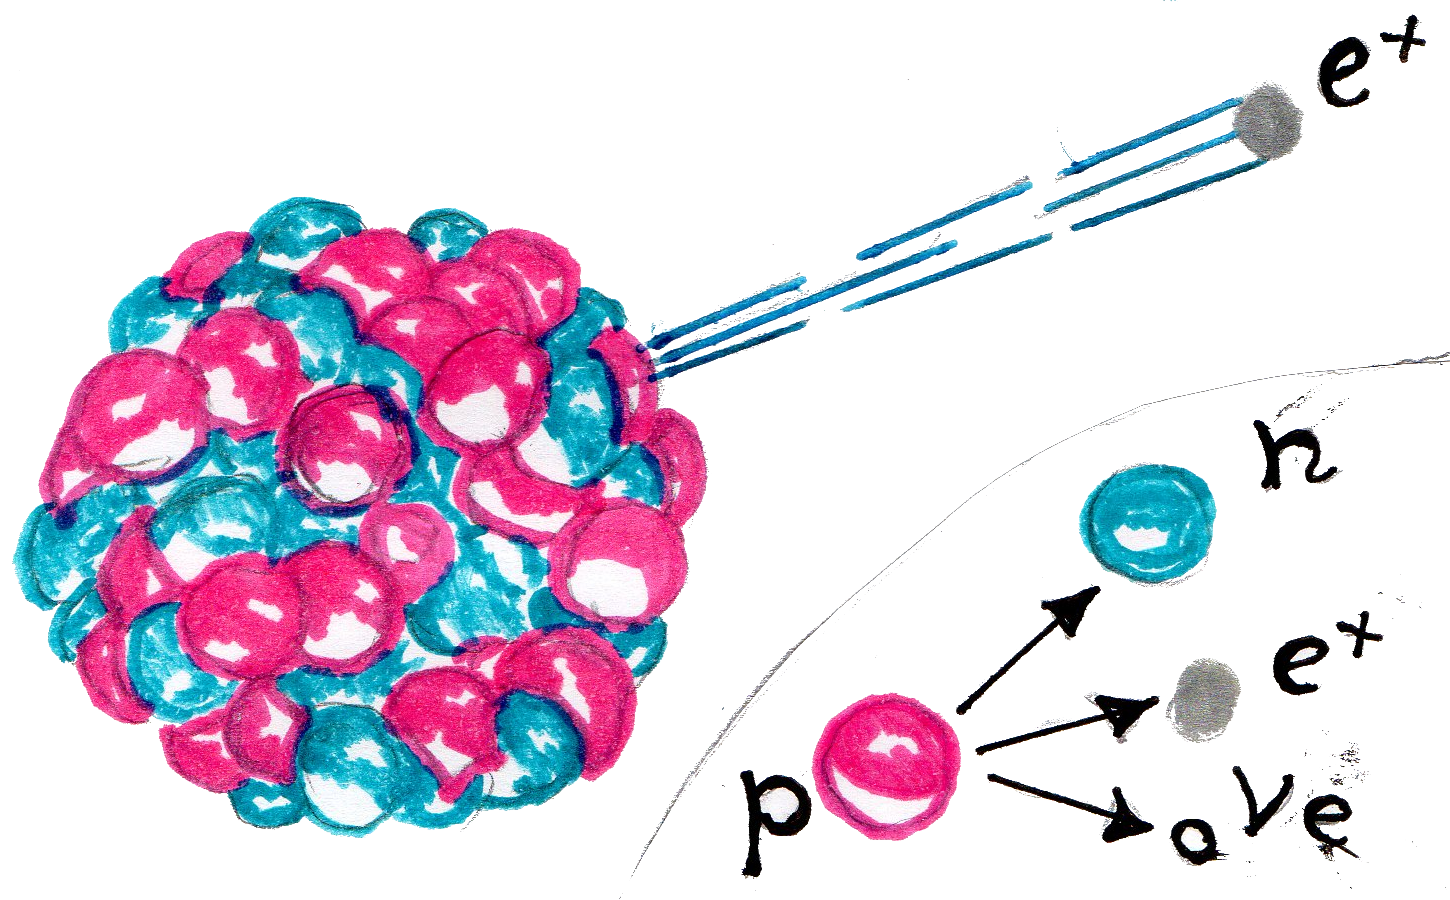
\includegraphics[width=1.0\linewidth]{figures/background_beta_plus_decay.png}
                    
                    \captionsetup{singlelinecheck=false, justification=raggedright}
                    \caption{Graphical example of $\beta+$-decay. Here in the top left of the figure a nucleus can be seen which is unstable as it has an imbalance of protons and neutrons. A positron can be seen exiting the nucleus as a byproduct of $\beta+$-decay converting a proton into a neutron. In the bottom right of the figure a closer example of this can be seen. Here it directly shows a specific proton and the neutron, positron and neutrino which are produced by $\beta+$-decay.} \label{fig:decay_and_annihilation_beta_plus_decay}
                \end{figure}
                
                \begin{figure}
                    \centering
                    
                    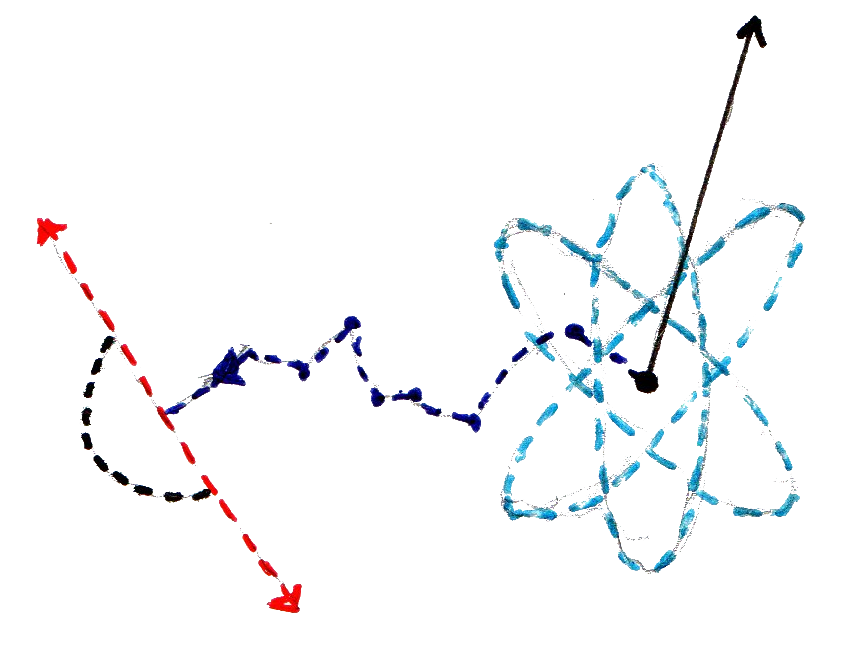
\includegraphics[width=1.0\linewidth]{figures/background_positron_range.png}
                    
                    \captionsetup{singlelinecheck=false, justification=raggedright}
                    \caption{Graphical example of positron range. Here on the right of the figure an atom can be seen travelling with some velocity, a positron is emitted from the nucleus of the atom by $\beta+$-decay. The path that this positron takes can be seen in the centre of the figure represented by a blue line, this path is the positron range. On the left of the figure the annihilation of the positron with an electron occurs and the $\gamma$-photons emitted $\SI{180}{^{\circ}}$ apart are shown.} \label{fig:decay_and_annihilation_positron_range}
                \end{figure}
                
                Radionuclides used in \gls{PET} undergo a type of decay called $\beta+$-decay~\boxcite{conti_beta}. This is due to an instability of the radionuclide, because of an imbalance in the number of neutrons to protons in the nucleus. As a consequence, a proton in the atoms nucleus is converted into a neutron subsequently releasing a positron and a neutrino, this can be seen in~\Fref{fig:decay_and_annihilation_beta_plus_decay}. The emitted positron travels with some decreasing velocity, because of sequential collisions, through the body of the patient, for a distance called its positron range, before it finally collides and annihilates with its antiparticle, the electron, this can be seen in~\Fref{fig:decay_and_annihilation_positron_range}~\boxcite{EvansPositronBib}. %KT citation probably not  needed
                
                The annihilation of positron and electron causes the emission of two $511$ \gls{KeV} $\gamma$-photons at $\approx\SI{180}{^{\circ}}$ apart from one another, thus travelling in approximately opposite directions. However, because the positron-electron pair may not be at rest at the moment of their annihilation, the two emitted photons can show a certain degree of non-collinearity, according to the laws of conservation of momentum. This means that the $\gamma$-photons are almost never exactly $\SI{180}{^{\circ}}$ apart~\boxcite{pet_basic}. %KT I'd cut the last sentence. repetition and you don't want to over-elaborate this
                %, because the positron will usually have a small kinetic energy going into the annihilation. This kinetic energy is conserved after the annihilation as a force in a different direction, usually, to that of the force from the annihilation itself.
                
                A \gls{PET} scanner thus does not image, directly, the emission of the positron but, in fact, more closely images the approximate location of its annihilation. %KT move this sentence down a bit %ACW done
            
            \subsubsection{Static and Dynamic Acquisition} \label{sec:static_and_dynamic_acquisition}
                There are two main types of \gls{PET} scan useful for determining separate processes. These types of scans and uses are:
                
                \begin{itemize}
                    \item The first and most common type of \gls{PET} scan is a static \gls{PET} scan~\boxcite{Muzi2012QuantitativeImaging}. The patient is scanned only when the injected radiotracer has distributed throughout their body and eventually approximately stabilised. %KT ``perfused'' is wrong. I'd say''distributed''. ``consistent'' sounds weird, so I'd say ``eventually approximately stabilised'' %ACW done, thank you
                    The time elapsed between injection and acquisition depends on the half-life and metabolisation of the radiotracer. For \gls{18F-FDG} about \SI{60}{\minute} is used.
                    
                    \item The second type of \gls{PET} scan is a dynamic scan. The acquisition of data for this scan begins before the radiotracer is injected into the patient. The injection of the radiotracer during the acquisition allows for the kinetics of the tracer to be observed and quantified with the use of compartmental modelling~\boxcite{Lammertsma2017}. For example, from dynamic \gls{PET} \gls{MPI}: %KT cut the ``direct parametric reconstruction'' here. not used in clinical practice. just say ``dynamic PET MPI''
                    in-vivo studies used in conjunction with tracer kinetic modelling enables the quantification of \gls{MBF}, often measured using rubidium-$82$. %Radiotracers such as rubidium $82$ are particularly indicated for dynamic scans given their short half life, seen in~\Fref{sec:decay_and_annihilation}. %KT doesn't have anything to do with halflife but with chemistry (calcium analogue). By the way, the ideal ``tracer'' to measure MBF is (radioactive) water! but that needs cycltron on site etc due to very short half-life. In contrast, Rb82 is produced in a generator. so say ``... MBF, often measured using Rb82.'' %ACW done, thank you, i didnt phrase the half life comment well, i mean that none perfusion or dynamic scans would be difficult with it
                \end{itemize}
            
            \subsubsection{PET Field of View} \label{sec:pet_field_of_view}
                \begin{figure}
                    \centering
                    
                    \includegraphics[width=1.0\linewidth]{figures/background_total_body_pet.png}
                    
                    \captionsetup{singlelinecheck=false, justification=raggedright}
                    \caption{Graphical representation of the difference between a total body \gls{PET} scanner and a standard \gls{PET} scanner. On the left of the figure a total body \gls{PET} scanner can be seen where the rings of detectors completely engulf the patient. However, on the right of the figure a standard \gls{PET} scanner can be seen where the rings of detectors only cover a portion of the patient. On the case on the right of the figure in order to take a scan over the entire body either individual acquisitions will be needed and concatenated or the bed would have to move while the acquisition was ongoing.} \label{fig:pet_fov_total_body_pet}
                \end{figure}
                
                The \gls{FOV} of the scanner is the area in which $\gamma$-photons can be detected. Current clinical \gls{PET} scanners, usually, have a cylindrical \gls{FOV} with a length of between \SI{15.0}{\centi\metre} and \SI{25.0}{\centi\metre} and a diameter of between \SI{50.0}{\centi\metre} and \SI{70.0}{\centi\metre}~\boxcite{Pan2019}.
                
                There are multiple ways to acquire data over more than the axial length of scanner, three of these methods are:
                
                \begin{itemize}
                    \item The most simple and widely used method is to take acquisitions over multiple bed positions and concatenate them.
                    
                    \item A method available on some  standard axial length scanners is; to continually move the bed through the rings of the scanner while acquiring data. This is advantageous as it is more comfortable for the patent and provides potentially less movement of the patient. %KT both these advantages can be done with the above step-and-shoot as well. I guess the advantages are patient comfort and potentially less moveemnt of the patient %ACW done
                    A disadvantage of this though is that it introduces another source of motion to the acquisition from moving the bed. This makes standard \gls{MC} much more difficult.
                    
                    \item Alternatively, total body \gls{PET} scanners are becoming more viable for research. %KT let's remove the ``high potential for  clinical applicatoin''. as you note below,price prevents this %ACW done
                    Total body \gls{PET} scanners have an axial \gls{FOV} which contains most of the patients body making multiple acquisitions less necessary while also increasing the sensitivity of the scanner, this can be seen in~\Fref{fig:pet_fov_total_body_pet}~\boxcite{Cherry2018}. However, the increased price and size constitute a limitation.
                \end{itemize}
            
            \subsubsection{Attenuation} \label{sec:attenuation}
                \begin{figure}
                    \centering
                    
                    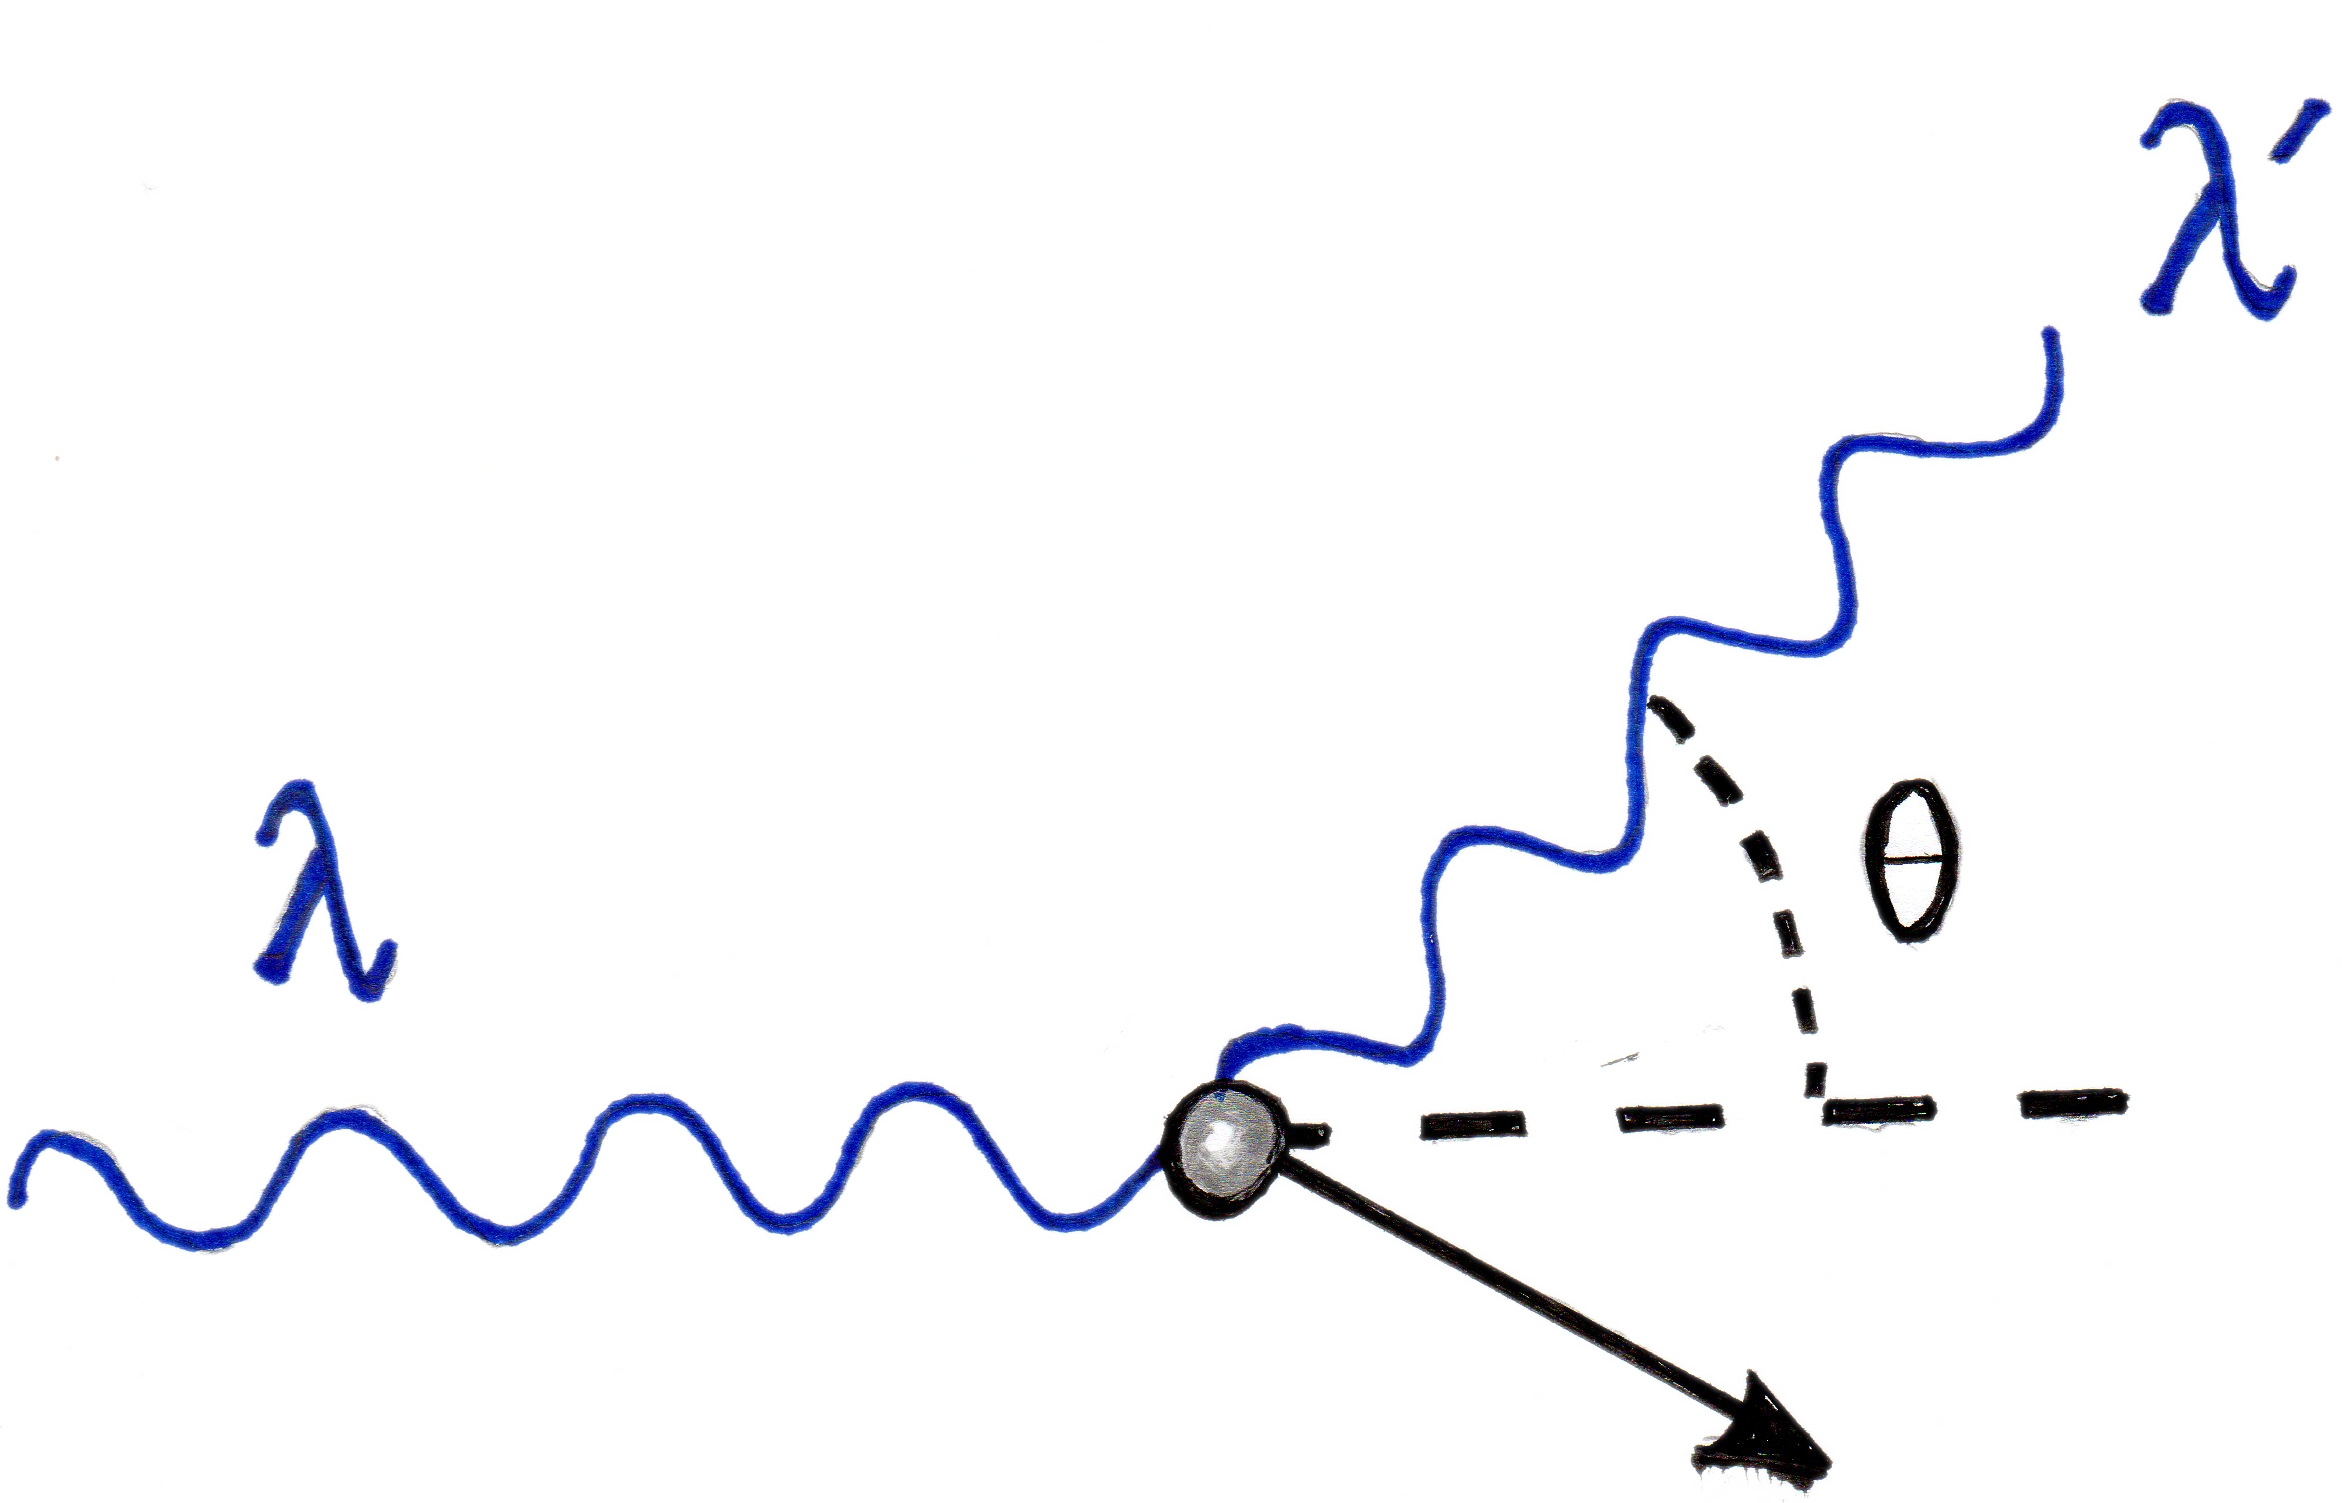
\includegraphics[width=1.0\linewidth]{figures/background_scatter.png}
                    
                    \captionsetup{singlelinecheck=false, justification=raggedright}
                    \caption{Graphical representation of a $\gamma$-photon scattering off of a particle. The $\gamma$-photon can be seen entering the figure on the left hand side before scattering off of a particle in the centre of the figure by an angle $\theta$ and exiting the figure on the top right hand corner. The particle exits the scatter event with some velocity represented by the arrow towards the bottom right. The trajectory of the $\gamma$-photon, had it not been scattered, is shown by the dotted line on the right hand side of the figure.} \label{fig:attenuation_scatter}
                \end{figure}
                
                %KT ``amount of counts'' is not correct. it's a process, or effect, not a number
                %ACW done
                %KT ``who quite literally...'' this doesn't read quite correct.I'd remove that part of the sentence
                %ACW done
                Attenuation is the process or effect through which counts are lost from annihilation to detection by the scanner while the photons are traversing through the body of the patient. Attenuation can amount to a loss of up to \SI{95.0}{\percent} of the total initial signal and can cause increased issues in larger bariatric patients~\boxcite{petspringer}~\boxcite{Essential2012}. %KT''book'' citation looks strange. missing space in the bibtex? also the guiberteau initials seem strange %ACW done
                
                There are three main ways through which the photon signal can be lost~\boxcite{scienceofpetspringer}, these are in ascending order of magnitude:
                
                \begin{itemize}
                    %KT this isn't a signal loss. I'd cut it (as it doesnt happen in PET)
                    %ACW done
                    %\item Pair production can be thought of as the inverse process compared to annihilation (as discussed above). This is where a subatomic particle and its antiparticle, such as a electron and a positron, are created from a fundamental particle, such as a photon, usually in close proximity to an atomic nucleus~\boxcite{Hubbell2006Electron-positronOverview}. However, because of conservation of energy a photon would need to be of at least $1.022$ \gls{MeV} which is not generally possible for photons created through electron positron annihilation.
                    
                    \item Rayleigh scattering is the elastic scattering of photons, without loss of significant energy, by particles which are much smaller than the wavelength of the photon. A common example of Rayleigh scattering is the scattering of sunlight in the atmosphere which causes the blue colour of the sky during the day and the red colour of the sky at sunset. Because the wavelength of $\gamma$-photons are comparably small, compared to most particles, the probability of Rayleigh scattering occurring is negligible and thus it is normally ignored in \gls{PET}.
                    
                    \item Absorption through the photoelectric effect is the process through which a high energy $\gamma$-photon hits and transfers its energy to a material causing the emission of lower energy electrons. The likelihood of the photoelectric effect is inversely proportional to the cube of the photon energy; it also increases as the atomic number of the attenuating material increases. In the matter of the patient the photoelectric effect is most prevalent at photon energies below $100$ \gls{KeV} and as such the probability of the photoelectric effect occurring for the \gls{PET} $\gamma$-photons is minimal~\boxcite{petspringer}. %KT ``here'' say instead ``for the PET gamma photons'' or so. phtoelectirc effect does occur for CT X-rays %ACW done
                    Attenuation through the photoelectric effect occurs mostly in the detectors of the scanner.
                    
                    \item Compton scattering comprises the majority of interactions between the photon and matter in \gls{PET}, it occurs where the photon interacts with an electron in a close by atom. The recoiling electron causes the photon to be deflected along another path transferring energy from photon to electron, this can be seen in~\Fref{fig:attenuation_scatter}. Compton scattering is also known as incoherent scattering. The probability of Compton scattering is indirectly proportional to the energy of the photon~\boxcite{petspringer}.
                \end{itemize}
                
                The relationship between the attenuation of the signal and the material through which it is travelling is given by the Beer-Lambert law. Given $I_0$ incident photons travelling across a path $D$, the number of non-scattered photons $\rmI_{\rmD}$ is given by: %KT given all of the above,I recommend to say ``the numberof  non-scattered photons...'' %ACW done
                 
                \begin{equation} \label{sec:eq:beer_lambert_law}
                    \rmI_{\rmD} = \rmI_{0} \cdot \exp\Bigg(\int_{\rmD} - \mu_E(r)\rmd r \Bigg) %KT why := ? %ACW done, because i wanted to be consistent
                \end{equation}

                \noindent where $\mu_E(r)$ is the attenuation coefficient of the media crossed by photons of energy $E$.
        
        \subsection{Data acquisition} \label{sec:data_acquisition}
            % write a general intro on the scanner structure, and the type of events you detect (true scatter randoms etc)
            
            \begin{figure}
                \centering
                
                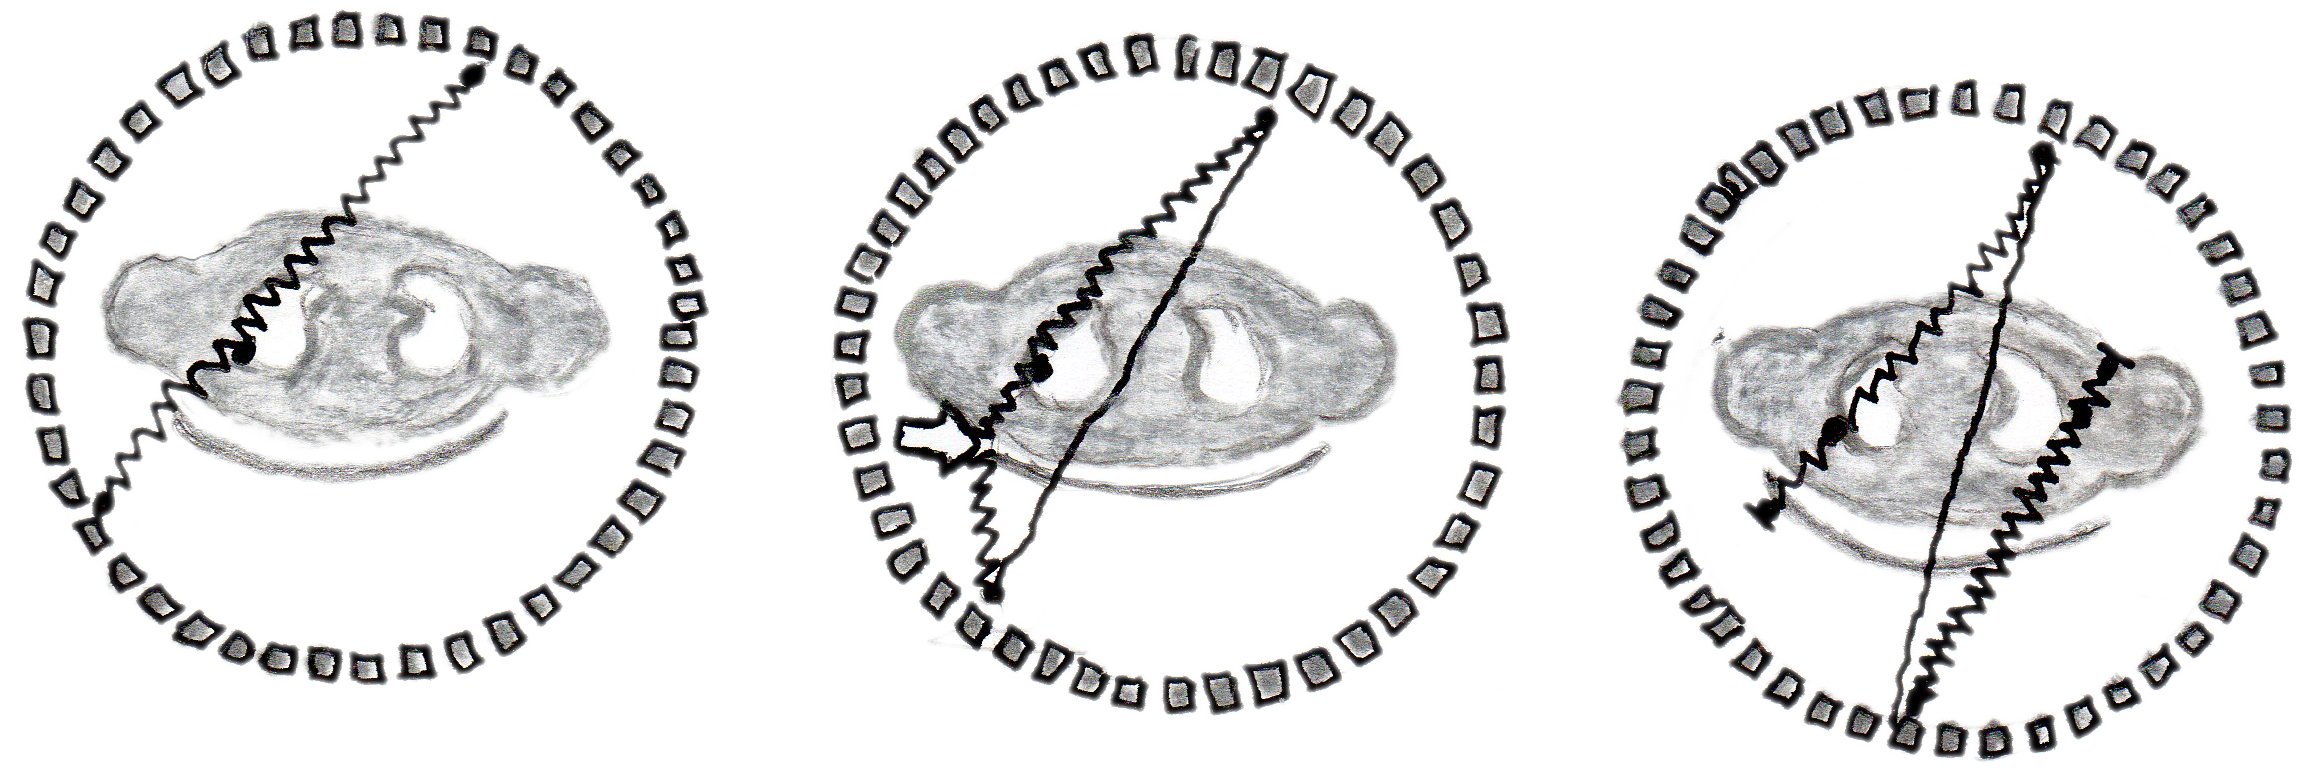
\includegraphics[width=1.0\linewidth]{figures/background_coincidence.png}
                
                \captionsetup{singlelinecheck=false, justification=raggedright}
                \caption{Graphical representation of the different types of coincidences possible in \gls{PET}. On the left of the figure a true coincidence can be seen, this is where the $\gamma$-photons from one annihilation are both detected without scattering. In the middle of the figure a scattered coincidence can be seen, this is where the $\gamma$-photons from one annihilation are both detected, however in this case one of them has scattered. On the right of the figure a random coincidence can be seen, this is where the $\gamma$-photons from two unrelated annihilations are detected.} \label{fig:data_acquisition_coincidence}
            \end{figure}
            
            As discussed in~\Fref{sec:pet_field_of_view}, the structure of a \gls{PET} scanner is that of concentric rings of detectors offset along a central axis. These rings detect each incident photon and attempt to temporally and spatially link opposing photons along a \gls{LOR} through the scanner. A \gls{LOR} being a line through the \gls{FOV} of the scanner linking two detectors. The methods through which the scanner attempts to %detect incident photons and then 
            link relative photons together will be discussed in the following %~\Fref{sec:photon_detection} and
            ~\Fref{sec:coincidence_processing}.
            
            Because of the photons interaction in matter shown in~\Fref{sec:attenuation}, there are four different types of event or coincidences that can be detected by the scanner, these are:
            
            \begin{itemize}
                \item Firstly, the coincidences that originate from the same annihilation event and pass through the body of the patient to the detector without being scattered or attenuated. These coincidences are called true coincidences as they approximately accurately reflect the position of the originating annihilation and thus the underlying activity distribution.
                
                \item Secondly, there are coincidences which may have originated from the same annihilation event but, from which one or more of the incident photons has undergone Compton scattering before detection. These coincidences are called scattered coincidences. Scattered coincidences can attempt to be corrected for if an accurate \gls{Mu-Map} is given, the density of the matter through which the photons must have travelled indicate the likelihood of scattering.
                
                \item Thirdly, there are coincidences where the \gls{LOR} is determined from two photons from two distinct annihilation events, thus the \gls{LOR} does not reflect an actual annihilation in reality. This could occur because one or more of the photons, from the original pair of photons, may have been attenuated or scattered so that it does not arrive at the detector within a reasonable time of its photon pair or that its \gls{LOR} doesn't go through one of the detectors. %KT  much more likely is that its LOR actually doesn't go through one of the detectors! (it's a 3D process of course) %ACW done
                These are called random coincidences. Random coincidences can be corrected for if acquisition data of this background level of the scan exists.
                
                \item Fourthly, there could be a situation where three or more photons are detected within close temporal proximity to one another. Because of the close time of detection, in this case it is not possible to determine which photons reflect an actual annihilation and which are random coincidences. These coincidences are called multiple coincidences. In normal procedures this is rare. %KT I recommend say that this is in normal procedures  rare. Otherwise an obvious viva question would be what people would do with them (as they're not in your equation below) %ACW done
            \end{itemize}
            
            An example of some of the types of coincidences from above can be seen in~\Fref{fig:data_acquisition_coincidence}.
            
            The total prompts detected during a \gls{PET} acquisition $P$ can be expressed as:
            
            \begin{equation}
                P := T + S + R
            \end{equation}
            
            \noindent where $T$ is the number of true coincidences, $S$ is the number of scattered coincidences and $R$ is the number of random coincidences. %Thus the usual total sum of scattered and random coincidences when compared to true coincidences is a ratio of $2$ to $1$. %KT this last sentence is incorrect. depends on count-rate, amount of scatter etc etc. Delete it %ACW done
            
%            \subsubsection{2D and 3D Acquisition} \label{sec:2d_and_3d_acquisition}
                %KT the 2D stuff reads as if in 2D PET there were collimators between all detectors, but in fact they were only between rings.
                %I highly recommend cutting this subsubsection. Detail not relevant to your work.
                %ACW depressingly done
%                \begin{figure}
%                    \centering
                    
%                    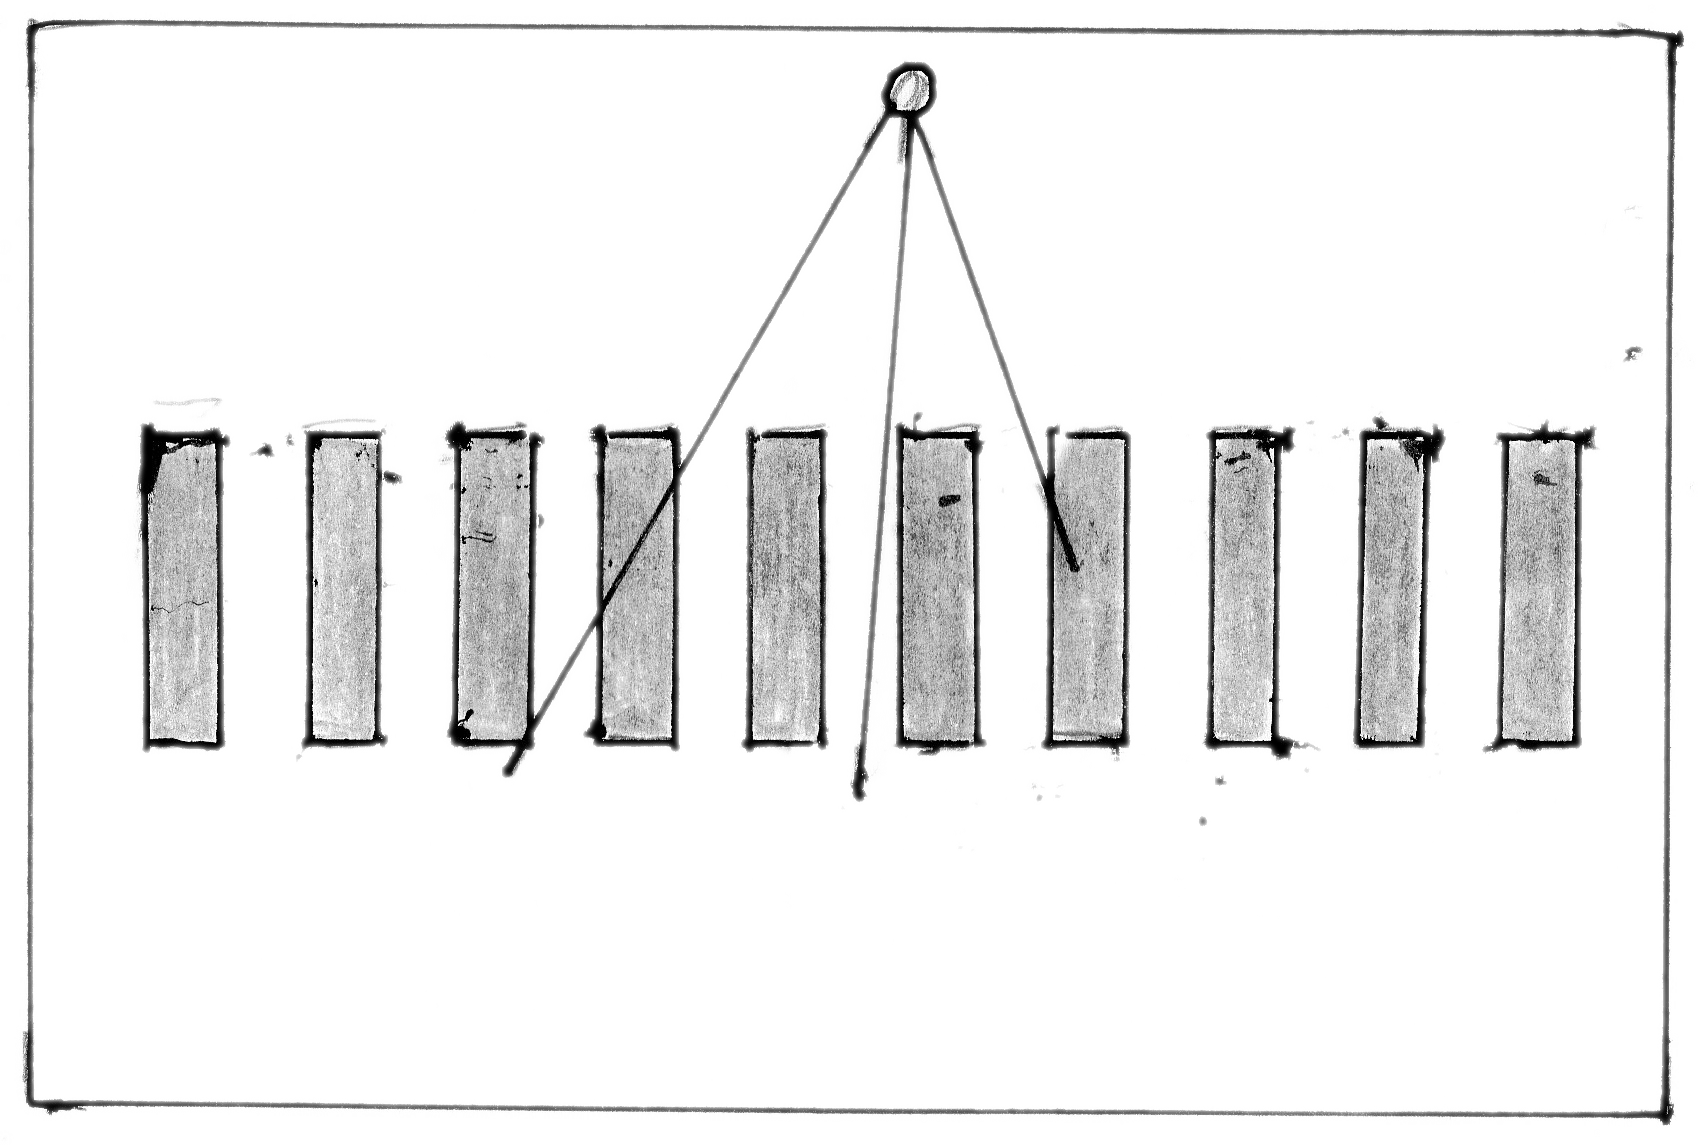
\includegraphics[width=1.0\linewidth]{figures/background_septa.png}
                    
%                    \captionsetup{singlelinecheck=false, justification=raggedright}
%                    \caption{Graphical representation of the cross section of the septa used for collimation in \gls{2D} \gls{PET} acquisitions. In this figure a point can be shown casting paths into the slits of the septa, as can be seen the paths from the point can only pass through the slits of the septa in positions where the angle of the line with respect the the walls of the septa is acute.} \label{fig:2d_and_3d_acquisition_septa}
%                \end{figure}
                
%                There are two different methods used in \gls{PET} to determine or constrain to be certain of the spatial position or angle of the \gls{LOR} along the axis of the scanner, these are:
                
%                \begin{itemize}
%                    \item The method which was used for a long time in other applications (such as \gls{SPECT}) and until recently in \gls{PET} was; to place a block of, usually, tungsten metal (for its photon absorbing properties) in front of all of the detectors, this block is called s septa, this can be seen in~\Fref{fig:2d_and_3d_acquisition_septa}. The septa has very small slits cut into it which would only allow photons to pass through which entered the slits at an acute angle. Thus the septa constrains the photons to being almost perpendicular to the detector (on axis) and as such each detector only receives signal from annihilations that occur within its ring. This process is called collimation and the subsequent acquisition is called a \gls{2D} acquisition, \gls{2D} not because it results in a single image but because it is comprised of distinct \gls{2D} projections.
                    
%                    \item The more modern method is to simply remove the septa from the scanner and to record coincidences between all rings. This is significantly more computationally expensive than a \gls{2D} acquisition but it also increases the sensitivity of the scanner meaning that scanning times can be reduced. Because this method produces projections between all rings it is known as a \gls{3D} acquisition~\boxcite{Schmitz2013}~\boxcite{Bailey1998ExperienceTomographs}.
%                \end{itemize}
            
%            \subsubsection{Photon Detection} \label{sec:photon_detection}
                %KT I did not read this. Far far too much detail for your thesis. I highly recommend commenting it out
                %ACW depressingly done
%                \begin{figure}
%                    \centering
                    
%                    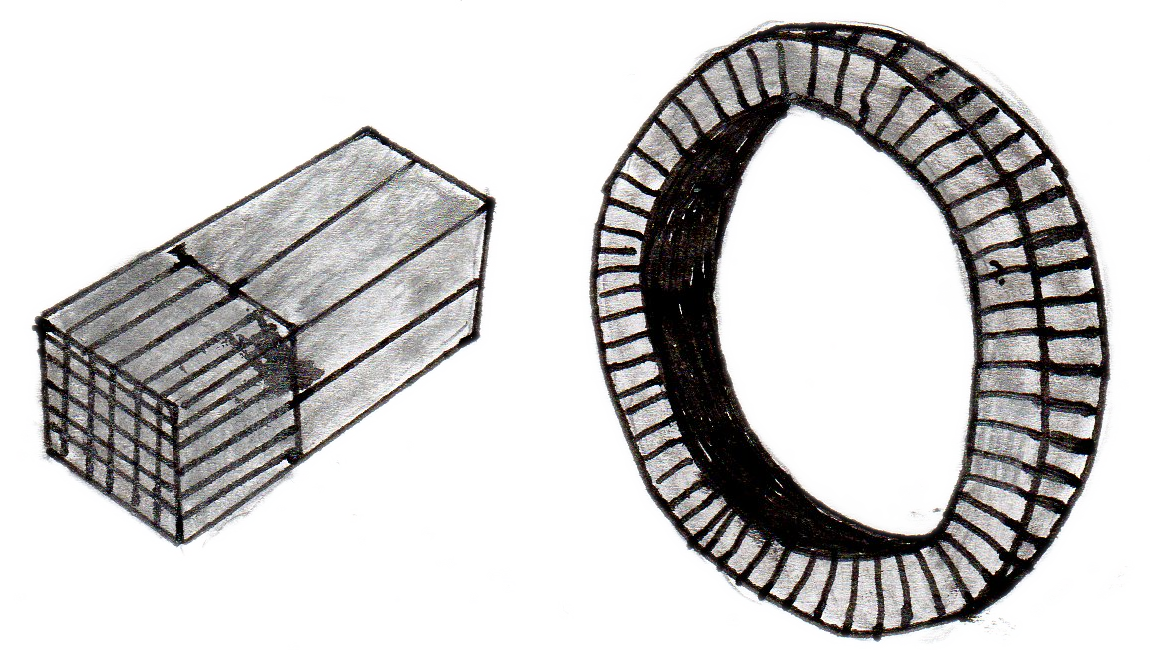
\includegraphics[width=1.0\linewidth]{figures/background_detector.png}
                    
%                    \captionsetup{singlelinecheck=false, justification=raggedright}
%                    \caption{Graphical representation of the block detector structure of the scintillator crystal and the photodetector (with multiple scintillator crystals per photodetector), on the left of the figure, and an example of how these block detectors would be combined to construct a ring of a \gls{PET} scanner, on the right of this figure.} \label{fig:photon_detection_detector}
%                \end{figure}
                
%                \begin{figure}
%                    \centering
                    
%                    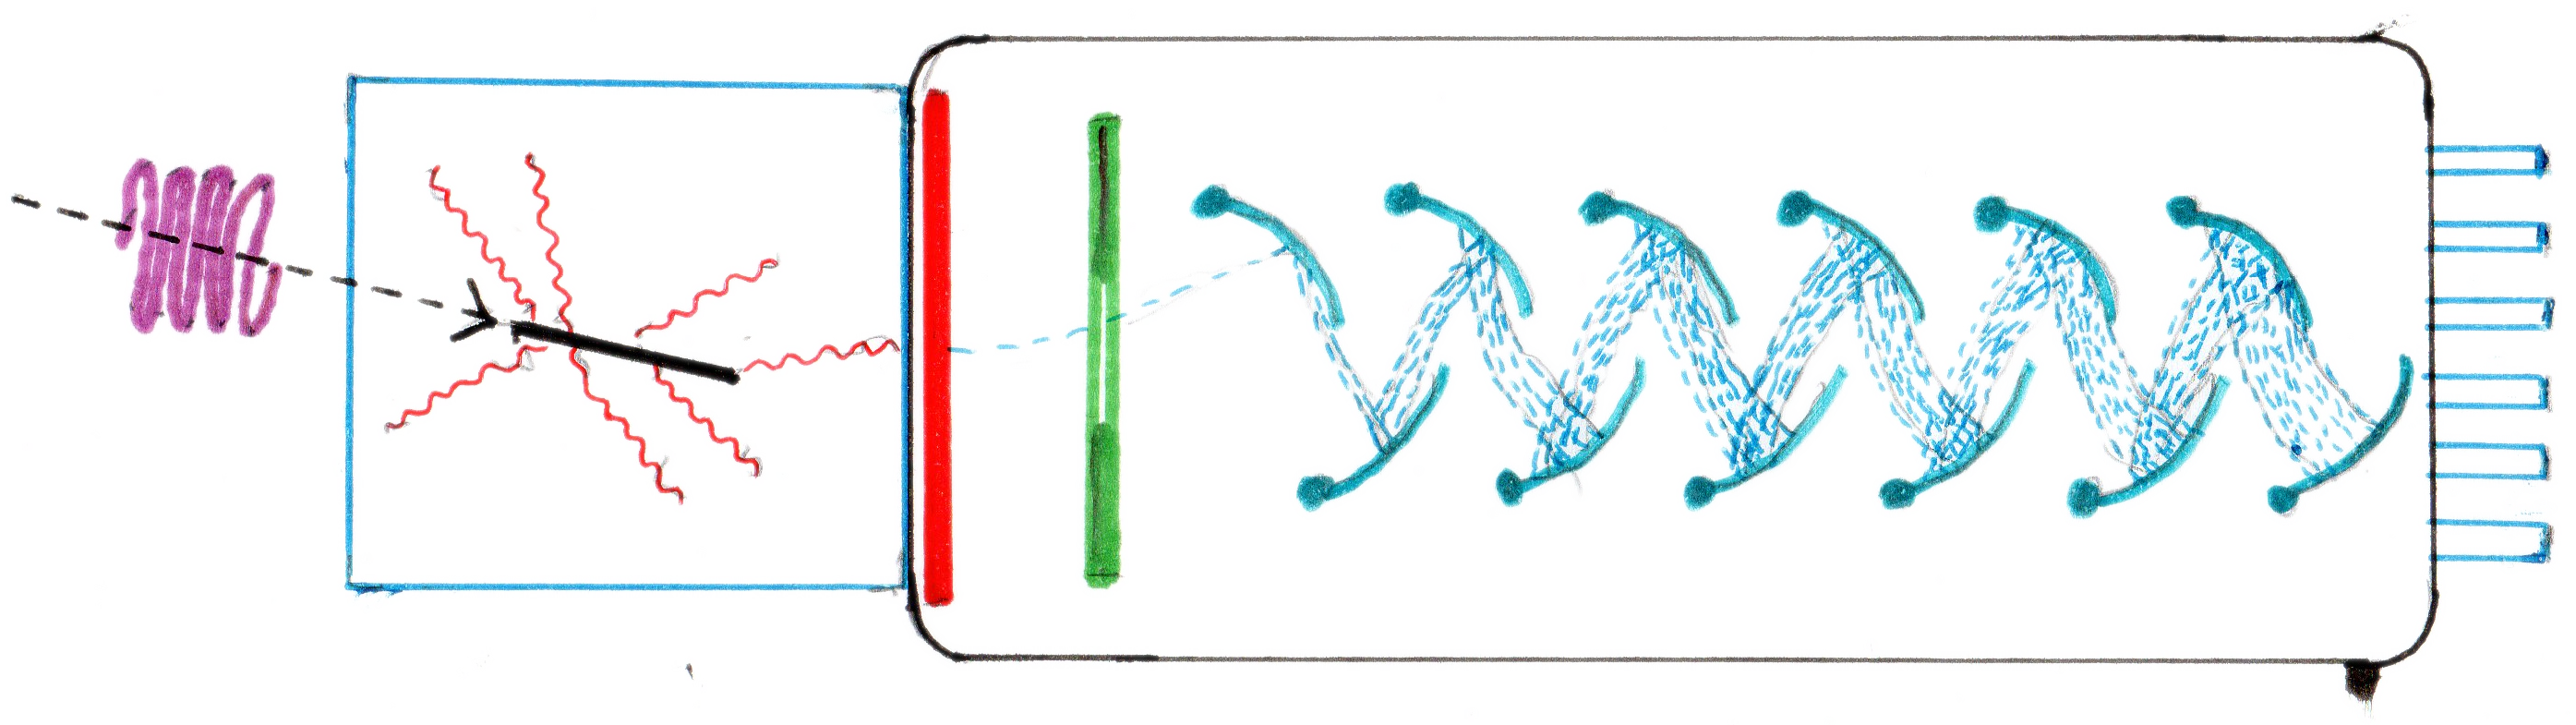
\includegraphics[width=1.0\linewidth]{figures/background_photomultiplier.png}
                    
%                    \captionsetup{singlelinecheck=false, justification=raggedright}
%                    \caption{Graphical representation of a scintillator crystal coupled to a \gls{PMT}. On the left of this figure a photon can be seen impinging upon the scintillator crystal and then being attenuated by the photoelectric effect at some depth. The electrons produced by this can then be seen, in the centre of this figure, interacting with the photocathode before being focused onto the first dynode. On the right of this figure, a naive representation, the amplification of the electrons can be seen by subsequent dynodes.} \label{fig:photon_detection_photomultiplier}
%                \end{figure}
                
%                PET detectors consist of two main components; a scintillator crystal, which, partially because of the photoelectric effect, when exposed to ionising radiation produces visible light through luminescence, and a photodetector or photomultiplier which amplifies the intensity of an input light similarly to how a vacuum tube or a transistor would amplify an electrical signal. These can be seen in~\Fref{fig:photon_detection_detector}.
                
%                For use in \gls{PET} the following properties are desirable for a scintillator crystal:
                
%                \begin{itemize}
%                    \item Firstly, the crystal should have a high stopping power. This means that the photon does not travel a great distance into the crystal before it undergoes attenuation by the photoelectric effect. Usually the higher the density of the scintillator crystal the greater the stopping power~\boxcite{Derenzo2003TheScintillator}.
                    
%                    \item Secondly, for each incident photon the scintillator should have a high light output. This not only means that the work photomultiplier will have to amplify the output less but it also means that discriminating between scattered and unscattered photons will be easier as the discrepancy between the output intensity of the two will be greater.

%                    \item Thirdly, the scintillator should return to a state where it can luminesce again rapidly after each incident photon. This means that more photons can be detected over time and that the exact moment a photon is attenuated can be better measured.
                    
%                    \item Finally, a scintillator crystal should not be hygroscopic. To be hygroscopic means that something has a tendency to absorb water.
%                \end{itemize}
                
%                The first \gls{PET} scanners used \gls{NaI} scintillator crystals before moving to \gls{BGO} and then to \gls{LSO} and \gls{LYSO}. Each new generation of scintillator crystals provided a different balance of the above characteristics. \gls{LSO} and \gls{LYSO} have the best combination of efficiency and time resolution while not being hygroscopic~\boxcite{BGOCherenkovBib}~\boxcite{ScintilatorsBib}~\boxcite{Mao2013CrystalCrystals}.
                
%                There are three main types of photodetector or photomultiplier, these are:
                
%                \begin{itemize}
%                    \item The first kind of photodetector to be used in \gls{PET} was the \gls{PMT}, this device functions using an initial photocathode and a focusing electrode which takes the output from the scintillator and directs it towards a chain of dynodes. Dynodes are an intermediate electrode which when struck by a photoelectron emit more photoelectrons at a more positive electrical potential through secondary emission. Each subsequent dynode is a a higher potential and emits more photoelectrons than the last causing the input signal to be amplified, this can be seen in~\Fref{fig:photon_detection_photomultiplier}. Some disadvantages of \glss{PMT} are that they are relatively bulky, are effected by a magnetic field and have a relatively low efficiency at approximately \SI{25.0}{\percent}~\boxcite{petspringer}~\boxcite{SiPmBib}.
                    
%                    \item To attempt to combat the low efficiency mentioned above the \gls{APD} was developed, this device utilises a semiconductor where there is a junction between positive and negative type silicone, this is similar to a traditional diode. This allows for efficiencies approaching \SI{85.0}{\percent}, they are much smaller than \glss{PMT} and are safe to be used in a magnetic field. However, this also comes with the drawbacks that \glss{APD} produces so much heat that it requires an active cooling system and exhibits worse timing characteristics than \glss{PMT}~\boxcite{AvalanchePhotodiodeBib}. \glss{APD} are the choice of many modern \gls{PET}/\gls{CT} scanners~\boxcite{Vandendriessche2019}.
                    
%                    \item A further development on \glss{APD} gave \glss{SiPM} and \glss{SSPM}. These devices combine the benefits of both \glss{PMT} and \glss{APD} in that they have a high efficiency, small size, are safe to be used in a magnetic field and have good timing characteristic. \glss{SiPM} and \glss{SSPM} are becoming the new default photodetectors in \gls{GE} scanners~\boxcite{SiPmBib}.
%                \end{itemize}
            
            \subsubsection{Coincidence Processing} \label{sec:coincidence_processing}
                % write stuff about coincidence processing , give some info on TOF (or separate section for it, i don't know)
                
                \begin{figure}
                    \centering
                    
                    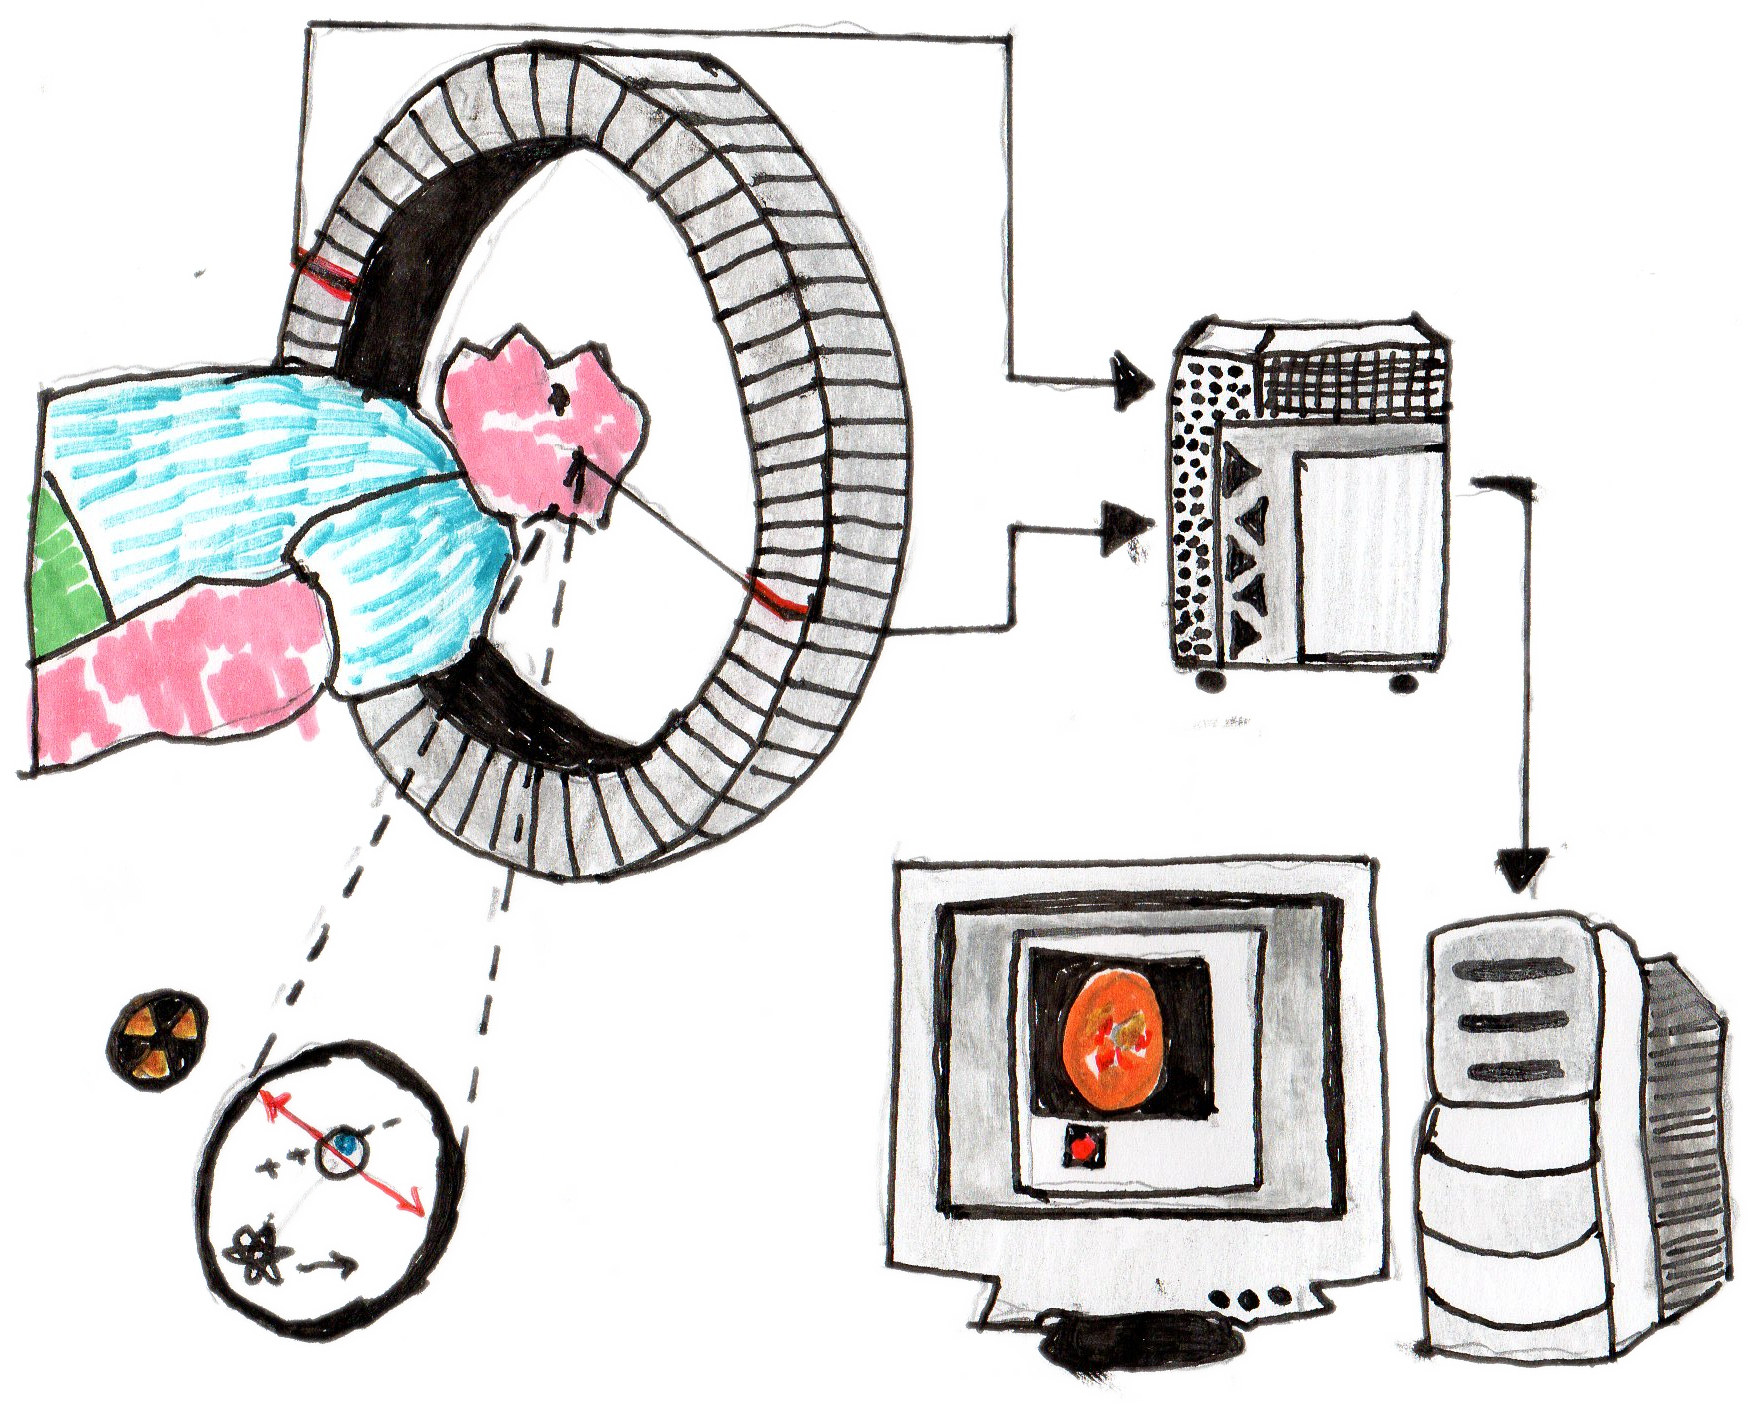
\includegraphics[width=1.0\linewidth]{figures/background_coincidence_processing.png}
                    
                    \captionsetup{singlelinecheck=false, justification=raggedright}
                    \caption{Graphical representation of the workflow from annihilation, to physical detection by the scanner, to then coincidence processing by the electronics of the scanner, before finally displaying some output to the user.} \label{fig:coincidence_processing_coincidence_processing}
                \end{figure}

                %KT first sentence sounds a bit weird. what does an LOR have to do with this? I'd shorten it.
                %ACW done
                %In order for a \gls{LOR} to be determined, the annihilation from which pairs of detected photons come from must be determined, in other words, they must be paired together in some way, as briefly mentioned above in~\Fref{sec:data_acquisition}.
                In order to form coincidences, the incident photons must be paired together to an annihilation event. First, before forming coincidences, the photons are filtered by selecting ones which only fall within an energy window of the scanner, for the \gls{GE} Discovery $690$/$710$ \gls{PET}/\gls{CT} this energy window falls approximately between $425$ and $600$ \gls{KeV}~\boxcite{Bettinardi2011}. Additionally, to attempt to determine temporally if two detected photons belong to the same annihilation event a coincidence window is used. If the events arrive more than the time of the coincidence window apart then they are determined to be unrelated. A standard coincidence window size would be about \SI{5.0}{\nano\second}. A naive representation of the workflow for coincidence processing can be seen in~\Fref{fig:coincidence_processing_coincidence_processing}.
            
            \subsubsection{Time of Flight PET} \label{sec:time_of_flight_pet}
                \begin{figure}
                    \centering
                    
                    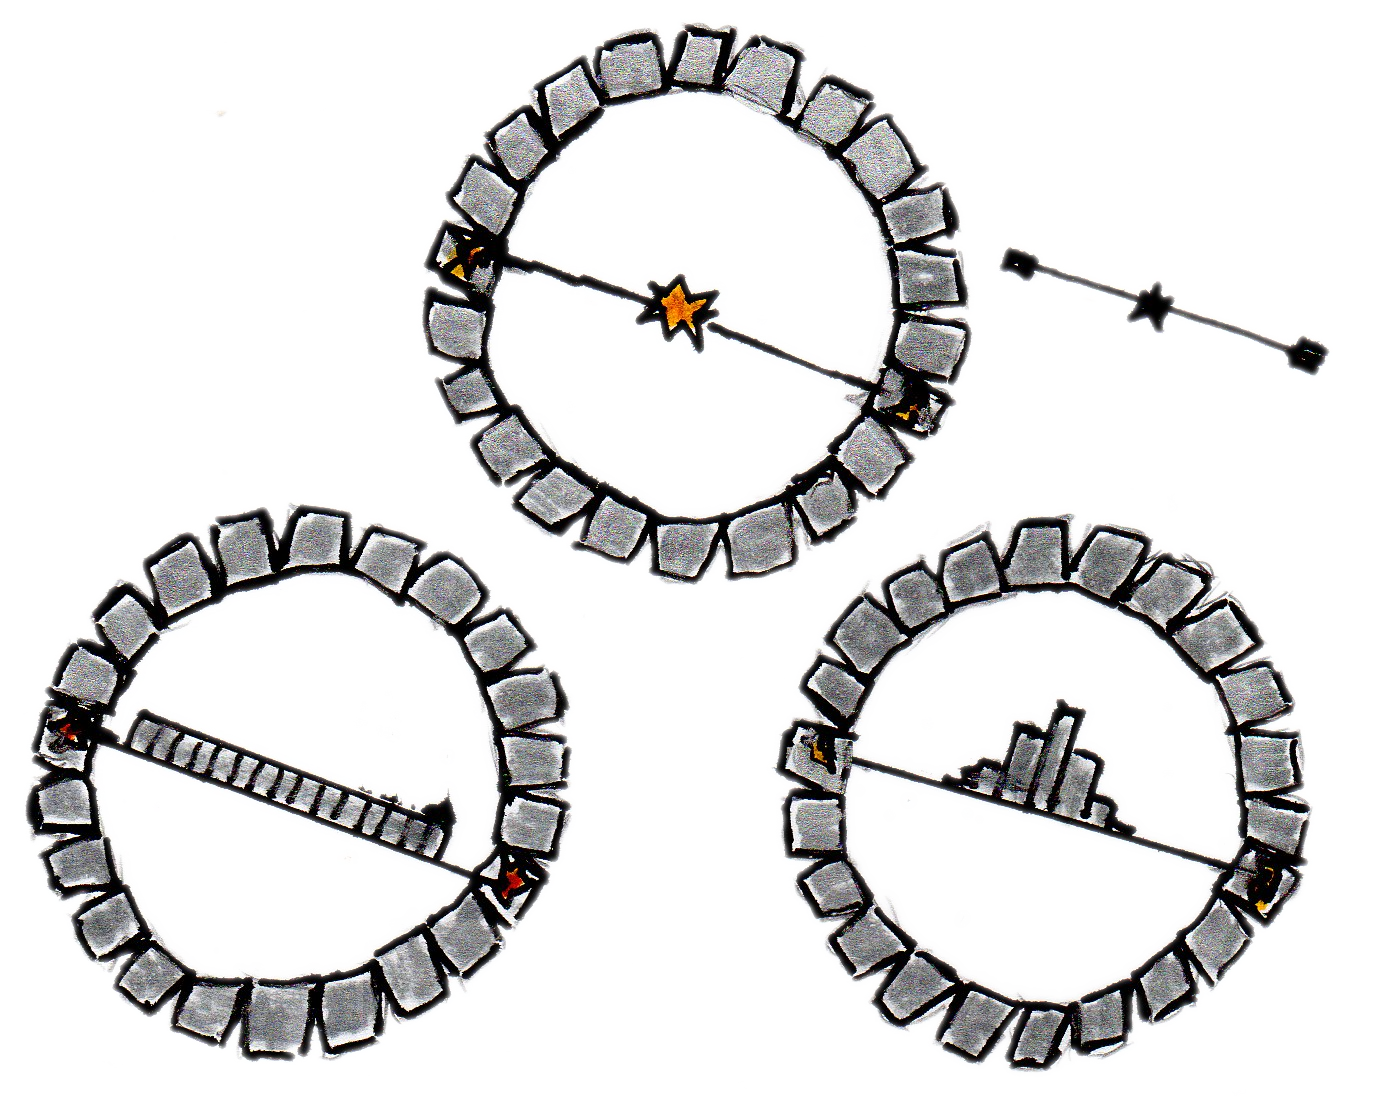
\includegraphics[width=1.0\linewidth]{figures/background_tof.png}
                    
                    \captionsetup{singlelinecheck=false, justification=raggedright}
                    \caption{Graphical representation of the concept of \gls{TOF}. The top middle of this figure shows the position where a hypothetical annihilation has occurred, plus the $\gamma$-photos from this annihilation which have then gone on to be detected by the scanner. The bottom left of this figure shows a traditional \gls{NTOF} acquisition where the probability of the position of the annihilation along the \gls{LOR} is constant. The bottom right of this figure shows a \gls{TOF} acquisition where the probability of the position of the annihilation along the \gls{LOR} can be approximated with a Gaussian based upon the difference in arrival time of both photons.} \label{fig:time_of_flight_pet_tof}
                \end{figure}
                
                \begin{figure}
                    \centering
                    
                    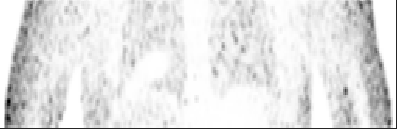
\includegraphics[width=1.0\linewidth]{figures/background_non_tof_example.png}
                    
                    \captionsetup{singlelinecheck=false, justification=raggedright}
                    \caption{Example of some \gls{NAC} \gls{NTOF} data, with noise, with no motion, randoms or scatters, of the thorax with a spherical lesion in the lungs. Coronal view.} \label{fig:time_of_flight_pet_non_tof_example}
                \end{figure}
                
                \begin{figure}
                    \centering
                    
                    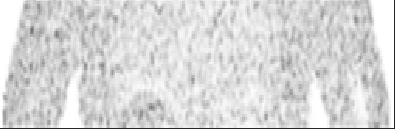
\includegraphics[width=1.0\linewidth]{figures/background_tof_example.png}
                    
                    \captionsetup{singlelinecheck=false, justification=raggedright}
                    \caption{Example of some \gls{NAC} \gls{TOF} data, with noise, with no motion, randoms or scatters, of the thorax with a spherical lesion in the lungs. Coronal view.} \label{fig:time_of_flight_pet_tof_example}
                \end{figure}
                
                As stated above in~\Fref{sec:coincidence_processing}, in order for the coincidence window based method to determine which specific detected photons represent \glss{LOR}, the scanner must be able to asses the difference in arrival time of each photon. %Because of this the scanner must record the absolute time at which it detects each incident photon. %KT delete previous sentence. it isn't really  necessary and essentially irrelevant anyway %ACW done
                It had been hypothesised for some time (since the $1960$s) that given the speed of light and the difference in arrival time at each detector, for each photon that makes a specific \gls{LOR}, then it should be possible to approximately calculate the position upon the \gls{LOR} at which a given annihilation occurred. %, known as \gls{TOF}. %KT ``know as TOF'' doesn't flow with the rest of the sentence %ACW done
                This can be seen in~\Fref{fig:time_of_flight_pet_tof}~\boxcite{Surti2015}~\boxcite{TOFPhotodetectorsBib}.
                
                The reason for the uncertainty of the position along the \gls{LOR} is because of the relatively course timing resolution of each given scanner. Generally modern \gls{PET}/\gls{CT} scanners have a timing resolution ranging between \SI{200.0}{\pico\second} and \SI{600.0}{\pico\second}, which represents an approximate spatial uncertainty of between \SI{30.0}{\milli\metre} and \SI{90.0}{\milli\metre}. %KT I think you forgot to divide by 2 %ACW done
                The uncertainty within these \gls{TOF} bins is usually modelled using a Gaussian distribution centred around the estimated position of annihilation by the scanner.
                
                %KT cut next paragraph. too much detail for you
                %ACW depressingly done
                %The timing resolution of the scanner is mainly dictated by the timing properties of both the scintillation crystal and the photodetector used. For the scintillation crystal, almost ubiquitously \gls{LSO} and \gls{LYSO} are used in modern \gls{PET} scanners which utilise \gls{TOF}. This is because they are the only scintillation crystals where they stop the photon and return to their base state post luminescence in a suitable time such that the time of arrival can be determined to any useful degree~\boxcite{TOFLSOBib}. For the photodetector, though \glss{PMT} possessed suitable timing properties to be used for \gls{TOF} now \glss{SiPM} and \glss{SSPM} are surpassing \glss{PMT} both in their timing properties and because they are not affected by magnetic fields and such can be used in both \gls{PET}/\gls{CT} as well as \gls{PET}/\gls{MR} scanners.
                
                Currently, \gls{TOF} is a focus for research because of the drastic improvements that it can have on the \gls{SNR}~\boxcite{Lecoq2017}~\boxcite{Cates2018}. %\gls{TOF} has such an impact on the resolution and reconstruction of \gls{PET} that it is used as a pseudo attenuation correction technique outside of the \gls{FOV} of the \gls{MR} in some \gls{PET}/\gls{MR} systems, such as the \gls{GE} Signa~\boxcite{Pan2019}. %KT I'd cut the previous sentence. This is  far more complicated than this (needs MLAA etc) %ACW done
                An example of some \gls{NAC} \gls{NTOF} and \gls{NAC} \gls{TOF} data can be seen in~\Fref{fig:time_of_flight_pet_non_tof_example} and~\Fref{fig:time_of_flight_pet_tof_example} respectively, notice the difference in distribution of counts in the centre of the thorax and lungs.
                
                The current (as of $2021$) \gls{PET}/\gls{CT} scanner with the highest \gls{TOF} resolution which is commercially available is the Siemens Vision with an approximate \gls{FWHM} of \SI{210.0}{\pico\second} or \SI{31.5}{\milli\metre}~\boxcite{VanSluis2019}. The \gls{PET}/\gls{MR} scanner with the highest \gls{TOF} resolution which is commercially available is the \gls{GE} Signa with an approximate \gls{FWHM} that is sub \SI{400.0}{\pico\second} or \SI{60.0}{\milli\metre}~\boxcite{SIGNA}~\boxcite{Hsu2017StudiesSystem}~\boxcite{Grant2016NEMASystem}~\boxcite{Caribe2019NEMAIsotopes}. %KT again factor 2in the mm %ACW done
            
            \subsubsection{Data Output} \label{sec:data_output}
                \begin{figure}
                    \centering
                    
                    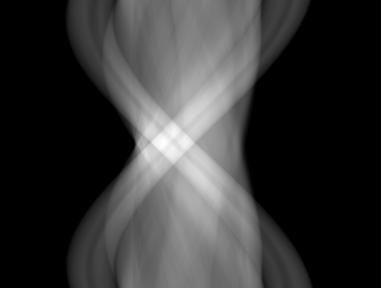
\includegraphics[width=1.0\linewidth]{figures/background_sinogram_data_example.png}
                    
                    \captionsetup{singlelinecheck=false, justification=raggedright}
                    \caption{Example of some simulated sinogram data, with no motion, noise, randoms or scatters, of the thorax with a spherical lesion in one of the lung.} \label{fig:data_output_sinogram_data_example}
                \end{figure}
                
                \begin{figure}
                    \centering
                    
                    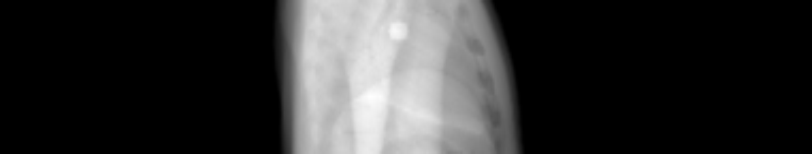
\includegraphics[width=1.0\linewidth]{figures/background_viewgram_data_example.png}
                    
                    \captionsetup{singlelinecheck=false, justification=raggedright}
                    \caption{Example of some simulated viewgram data, with no motion, noise, randoms or scatters, of the thorax with a spherical lesion in one of the lung.} \label{fig:data_output_viewgram_data_example} %KT fine, but it hardly shows what it's a sinogram (as you used a viewgram). maybe show both? %ACW done
                \end{figure}
                
                The output from a \gls{PET} scanner must be stored in a %universally understood
                file format in order to be of any use. %KT not true (in theory, but also not in practice. As long as the manfacturer can read it, they're fine...) %ACW done
                This file format will usually contain information related to the prompts from the acquisition, discussed above in~\Fref{sec:data_acquisition}. Each prompt stored represents a \gls{LOR} connecting the centre of two detectors. %KT probably first time you define LOR, while used multiple times above %ACW done
                Where \gls{TOF} information is available it is stored as an extra dimension in this file. This file can then be taken and reconstructed in order to estimate the original distribution of the radiotracer, this will be discussed later in~\Fref{sec:pet_image_reconstruction}.
                
                There are two main formats in which this information is stored from the scanner:
                
                \begin{itemize}
                    \item The most common way, that is used in clinical practise, is a format called a sinogram. During acquisition, if a sinogram output is specified, then the coincidences detected by the scanner are binned into a histogram which represents their plane orthogonal to the scanner, their orientation angle, their average axial location and their distance from the centre of the gantry. \gls{TOF} can be added as an additional dimension if it is used. %KT and TOF... %ACW done
                    If a single point source were imaged it would produce a sinusoid when binned into a sinogram, hence the name. An example of sinogram (where the \gls{LOR} are in a given transaxial plane) and viewgram (where the \gls{LOR} are along a given view, parallel to each other) data, with no noise, can be seen in~\Fref{fig:data_output_sinogram_data_example} and~\Fref{fig:data_output_viewgram_data_example} respectively. Because data is being binned into a histogram with this method, information is lost, it could be considered a lossy compression method.
                    
                    \item A less common method but one which is becoming more prevalent is a format called listmode data. Here each coincidence is recorded sequentially in a file. The information stored for each coincidence includes its arrival time, the coordinates of the detector and its detected energy. \gls{TOF} information can also be stored if it is used. %KT what do you mean with ``and coincidence''. don't forget TOF info... %ACW done
                    A listmode file can be directly reconstructed or first unlisted into a sinogram post acquisition. %Because a listmode file does not compress the output from the scanner, such as by binning the data into a histogram like with a sinogram, then the size of a listmode file will always be inherently larger than an equivalent sinogram. %KT cut previous sentence. it's not correct because of 2 reasons. If you have only 2 counts, the listmode file will be shorter. Siemens does compress info in the listmode file (to save space) %ACW done
                \end{itemize}
            
            \subsubsection{PET resolution} \label{sec:pet_resolution}
                There are five main effects which impact the resolution of a \gls{PET} acquisition, these are:
                
                \begin{itemize}
                    \item Firstly, there is, as has been discussed above in~\Fref{sec:decay_and_annihilation}, the effect of positron range. Because the positron travels a small distance before undergoing annihilation the \gls{PET} scanner will always, at best, be measuring the position of the annihilation rather than the position of the decay and as such not directly measuring the position of the radiotracer~\boxcite{PositronRangeLevinHoffmanBib}.

                    %KT ``as discussed''. exactly. so cut most of the remaining text!
                    %ACW done
                    \item Secondly, again as discussed above in~\Fref{sec:attenuation}, acollinearity of the $\gamma$-photons introduces errors which affect the resolution of \gls{PET}. %because the positron will almost always enter the annihilation event with some velocity then the $\gamma$-photons produced will exit with the same additional velocity. This velocity is also almost always in a direction other than that which the $\gamma$-photon would otherwise travel in, this causes the photons to travel in a direction which is not exactly $\SI{180}{^{\circ}}$ apart from one another.
                    This effect is exacerbated by the amount of time that the photons are allowed to travel, thus the larger the bore of the \gls{PET} scanner the larger this effect will have on the resolution. The effect of acollinearity on \gls{18F-FDG} gives an error of approximately $\SI{0.54}{^{\circ}}$~\boxcite{AccollinearityBib}
                    
                    %\item Thirdly, the size of each detector dictates the angular resolution of the scanner, %KTangular?
                    %or the number of \gls{LOR} covering any $\SI{360}{^{\circ}}$ slice is directly proportional to the number of detectors in each ring. Thus the resolution at which you can reconstruct before the sparsity of the \gls{LOR} means that some voxels will have zero \gls{LOR} passing through them is determined by the size of each individual detector~\boxcite{Nieman2015}. %KT I don't understand at all what you're trying to see with the rest of this. cut! %ACW done
                    
                    \item Thirdly, the block construction of each detector negatively impacts the resolution. This is because a number of scintillation crystals is paired with, usually, fewer photodetectors%, this can be seen in~\Fref{fig:photon_detection_detector}
                    . This means if a photon interacts with one crystal it may incorrectly be attributed to another crystal~\boxcite{Nieman2015}. So called digital \gls{PET} scanners are beginning to be seen which use a $1:1$ ratio of photodetectors to scintillation crystal, effectively removing issues related to block construction~\boxcite{Schillaci2019DigitalImaging}.
                    
                    \item Finally, %as discussed in~\Fref{sec:photon_detection}, 
                    a scintillation crystal has some stopping power, this power describes the approximate depth at which photons will undergo attenuation by the photoelectric effect. In some instances, depending upon the position and angle at which the incident photon hits the scintillation crystal it is possible for the photon to travel through the crystal and into an adjacent crystal before being detected. This means that the photon is incorrectly positioned and will result in blurring of the reconstructed volume~\boxcite{Nieman2015}.
                \end{itemize}
        
        \subsection{Combined PET/CT} \label{sec:combined_pet_ct}
            A \gls{CT} scanner consists of two devices which sit one on either side of the bore of the scanner. %KT ``straight parallel''? cut
            One device is an X-ray emitter and the other is an X-ray detector. If the X-ray emitter were to operate in one fixed position the result would be similar to a standard diagnostic X-ray, the difference comes in that for \gls{CT} during a continuous acquisition the device moves around the axis of the scanner taking continuous measurements. This allows for an X-ray image at every angular position. While the \gls{CT} is acquiring, the bed of the scanner travels along the axis of the scanner, %KT doesn't  make sense if you think about. instead, it's the bed that's moving %ACW done
            this allows for the collection of data over a \gls{3D} volume (similar as to what \gls{PET} collects over). This method of acquiring \gls{3D} data by taking measurements at a number of angles or section around a subject using a penetrating wave is known as tomography and is the same as the tomography of \gls{PET}.
            
            When the X-ray beam intersects with the body of a patient it is possible for the beam to be attenuated by the photoelectric effect or scattered,%KT also Compton %ACW done
            similarly to discussed in~\Fref{sec:attenuation}. Where the intensity of the beam detected is less then it can be assumed that there is a higher density object attenuating more of the beam between it and the emitter. If this information is collected over a \gls{3D} volume it allows for the generation of a \gls{3D} volume that reflects the attenuation of the body of the patient, for instance. This attenuation is normally expressed in \glss{HU}.
            
            The energy of the X-ray used in \gls{CT} consists of many different wavelengths, hence it is polychromatic. The wavelength range usually used in a \gls{PET}/\gls{CT} acquisition is between $40$ and $140$ \gls{KeV}~\boxcite{CTattenuationenergyBib}. The wavelength range is determined by the settings of the scanner, these mainly consist of the peak \gls{KV} and the electric current applied, in \SI{}{\milli\ampere}.
            
            In a standard \gls{PET}/\gls{CT} scan the \gls{CT} component comes first before the \gls{PET}. In modern \gls{PET}/\gls{CT} scanners the \gls{CT} and \gls{PET} are inline with the same bed, however the first \gls{PET}/\gls{CT} scans were taken on different machines entirely and as such the position of the patient differed more drastically between scans. A standard \gls{CT} scan over the thoracic region specifically will last approximately between \SI{2.0}{\second} and \SI{3.0}{\second}~\boxcite{PETCTImagingTechnicalConsiderationsBib}.
        
            \subsubsection{Attenuation Correction} \label{sec:attenuation_correction}
                \begin{figure}
                    \centering
                    
                    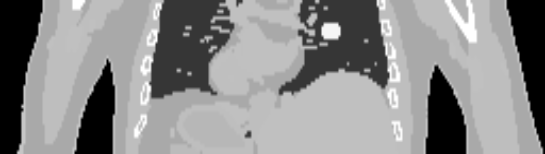
\includegraphics[width=1.0\linewidth]{figures/background_mu_map_example.png}
                    
                    \captionsetup{singlelinecheck=false, justification=raggedright}
                    \caption{Example of a simulated \gls{Mu-Map}, with no motion or noise, of the thorax with a spherical lesion in the lungs. Coronal view.} \label{fig:combined_pet_ct_mu_map_example}
                \end{figure}
                
                \begin{figure}
                    \centering
                    
                    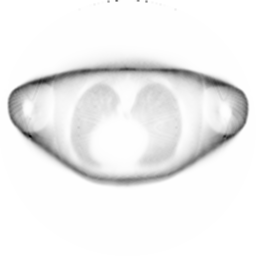
\includegraphics[width=1.0\linewidth]{figures/background_nac_example.png}
                    
                    \captionsetup{singlelinecheck=false, justification=raggedright}
                    \caption{Example of simulated \gls{NAC} \gls{TOF} data, with motion, with no noise randoms or scatters, of the thorax with a spherical lesion in the lungs. Transverse view.} \label{fig:combined_pet_ct_nac_tof_example}
                \end{figure}
                
                \begin{figure} %KT if you're bored (!),I'd put the NAC and AC figures next to eachother
                    \centering
                    
                    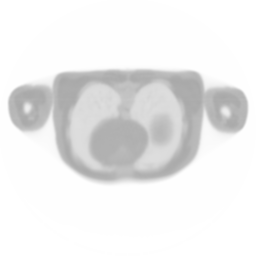
\includegraphics[width=1.0\linewidth]{figures/background_ac_example.png}
                    
                    \captionsetup{singlelinecheck=false, justification=raggedright}
                    \caption{Example of simulated \gls{AC} \gls{NTOF} data, with motion, with no noise, randoms or scatters, of the thorax with a spherical lesion in the lungs. Transverse view.} \label{fig:combined_pet_ct_ac_tof_example}
                \end{figure}
                
                As discussed previously in~\Fref{sec:attenuation} attenuation represents the loss of coincidences by photon interactions in matter. Attenuation is an issue in \gls{PET} as it causes the loss of signal and a degradation in image quality, this is the opposite for \gls{CT} where the modality itself relies on attenuation in order to differentiate anatomical structure, an example of a \gls{Mu-Map} can be seen in~\Fref{fig:combined_pet_ct_mu_map_example}. An example of some \gls{NAC} \gls{TOF} and \gls{AC} \gls{TOF} data can be seen in~\Fref{fig:combined_pet_ct_nac_tof_example} and~\Fref{fig:combined_pet_ct_ac_tof_example} respectively. In order to find reasonable quantitative results the attenuation of the patient must be taken into account in \gls{PET}. %Both \gls{PET} and \gls{CT} follow the Beer-Lambert law. %KT cut last sentence.not  relevant here %ACW done
                
                Methods to acquire \gls{Mu-Map}, for \gls{AC} include; to take a transmission scan of a known point source rotated around the body of the patient prior to the injection of the radiotracer. This allows for the estimation of the attenuation for each angle~\boxcite{TransmissionatnBib}. Another method involves the use of the known attenuation from the \gls{CT} scan.
                
                In order to apply the \gls{CT} based \gls{Mu-Map} to \gls{AC} in \gls{PET} first it must undergo either bilinear or trilinear conversion to asses the attenuation coefficient factors, this is because of the relative energy difference of the two modalities~\boxcite{Carney2006}. As discussed above in~\Fref{sec:coincidence_processing} and~\Fref{sec:combined_pet_ct} \gls{PET} and \gls{CT} operate at two different energy levels of between between $425$ and $600$ \gls{KeV} and between $40$ and $140$ \gls{KeV} respectively~\boxcite{Bettinardi2011}~\boxcite{CTattenuationenergyBib}.
                
                Issues with \gls{CT} based \gls{AC} include: Firstly, as mentioned above in~\Fref{sec:combined_pet_ct}, \gls{CT} is acquired sequentially to \gls{PET} rather than simultaneously meaning that there can be mismatches in anatomy between the scans. Secondly, the propagation of any artefacts from the \gls{CT} volume into the \gls{PET} volume. Regardless of these issues \gls{CT} is currently considered to be the gold standard for \gls{Mu-Map} estimation for \gls{AC}. Transmission scans are now very rarely used because of the inclusion of an additional external source, their significant increase in scan time and low image quality compared to \gls{CT}. 
                %KT  Briefly mention MLAA here
                %ACW done
                
                Recently a method to jointly estimate both the activity and attenuation distributions from \gls{PET} data only has been proposed called \gls{MLAA}. This method attempts to reconstruct both distributions by iteratively estimating one distribution while keeping the other one fixed. This can be considered as at each step performing either emission or transmission tomography depending on the distribution being optimised for%. Alternatively, it is also possible to optimise jointly for both distributions in one step
                ~\boxcite{Fuin2017}~\boxcite{Brusaferri2019}. A disadvantage of this solution is that without \gls{TOF} information it is a highly ill-posed problem and even with \gls{TOF} data the solution can only be found up to an arbitrary scaling factor. It is also possible for there to be significant cross talk artefacts between the activity and attenuation estimate~\boxcite{MLAASalomonBib}~\boxcite{MLAADefriseBib}. Additionally, optimising for the attenuation distribution increases the complexity and computational effort required of a reconstruction algorithm.
                
    \longsection{Inverse Problems and Optimisation}{sec:inverse_problems_and_optimisation}
        This section of the thesis introduces the concept of inverse problems. First a definition of an inverse problem is given, including where these may be applicable to the field of \gls{PET}. Next, the definition of an inverse problem is expanded upon by highlighting the difficulty of solving them literally and how this is usually overcome or addressed. The general form of an approach to solving an inverse problem is then given.
            
        The second subsection expands upon the approach given previously to solving inverse problems. Including; defining what an optimisation is, applications of optimisation (for instance, \gls{PET} reconstruction) and listing the requirements of a simple optimisation problem. Next this subsection moves onto addressing the components of an optimisation, including the objective function. The purpose of an objective function in optimisation is presented before a number of common and robust similarity measures are introduced, the merits of different functions is discussed and common applications of specific instances is given. Regularisation is then briefly mentioned before moving onto the optimiser. As with the previous subsection here the purpose of an optimiser is initially introduced before families of optimisation algorithms are compared and variations of these families, as well as their applications, are touched upon. Finally bounds or constraints upon optimisation are mentioned, as well as providing examples of optimisers which can incorporate such functionality.
        
        \subsection{Inverse Problem Concepts} \label{sec:inverse_problem_concepts}
            An inverse problem is one where the original conditions of a system are approximated from its effects. For instance, the data from a \gls{PET} scanner represents the observations of the distribution of the radiotracer, reconstruction is an attempt to find the distribution from these observations.
            
            It is not usually possible to directly invert a problem like this, often due to the complexity or size of a problem (meaning that  the computation time to find an inverse would be large). Thus in these cases the solution can be iteratively optimised for. In order to attempt to find the solution to an inverse problem there are two things which are required; first the forward operator (the forward operator describes the problem in the direction of its initial conditions to its effects) %KT true, but do you understand this? simplify by cutting %ACS I'm pretty sure I do now
            second, ideally, a model of the noise present in the system~\boxcite{Brusaferri2020ImprovingInformation}~\boxcite{Emond2020ImprovingEffectiveness}. %KT what ``at least''. I'd say ``ideally'' %ACW done
        
        \subsection{Optimisation Concepts} \label{sec:optimisation_concepts}
            Optimisation means to find values that best parametrise a given function based on some criteria or objective. %KT I feel it needs something else ``based on some criteria'' or ``objective'' or ... %ACW done
            For instance, in reconstruction an optimisation could be to find the image that when the forward operator is applied to it the result best matches the measured data. Another example of an optimisation would be to find the motion parameters that when applied to a given image most closely warp that image to match another image. Optimisation is also used in fields such as deep learning to train neural networks, here the optimisation is used to find parameters for a model that maps one set of values to another.%, this will be discussed later in~\Fref{sec:machine_learning_for_pet}.
            
            In order to perform a basic optimisation four components are required; most importantly an objective function (which returns the goodness of the current estimate) and a method to optimise the estimate based on this function are paramount. Additionally, an initial estimate (the closer this is to the ideal estimate then the less computation time is required overall) and a method to determine when optimisation should cease (for instance when the objective function exceeds a threshold or the number of iterations becomes so large) are also necessary. These will be discussed in the following sections in~\Fref{sec:objective_function} and~\Fref{sec:optimiser} respectively.
        
            \subsubsection{Objective Function} \label{sec:objective_function}
                Optimisation of some values requires a function that represents, for instance, the similarity of two measures or the likelihood given a measure. This function is necessary as its output reflects the accuracy of the current estimate. The gradient of the objective function describes the direction in which the optimiser should change the estimate. The optimiser attempts to find a solution by either maximising or minimising the result of applying the objective function and updating the estimate iteratively.
                
                An example of an objective function would be \gls{MAE}. For a vector of some values, \gls{MAE} subtracts the estimated value from the true value, finds the absolute value of this and sums together this value for all values in the vector. The absolute value is taken because the error should be the distance to the true value regardless of if the estimated value is greater or less than the true value. If the estimated values approach the true values then the value of the \gls{MAE} will approach zero. If \gls{MSE} is used then the square of the error is taken rather than the absolute value, taking the square causes the error to increase quadratically as it becomes larger. %KT exponentially? no,quadratically %ACW done
                This can be advantageous as it penalises large errors more than smaller ones, which can lead to a better result in some circumstances. Additionally, the square is differentiable.
                
                More complex objective functions include; \gls{RMSE}, here the square root of \gls{MSE} is taken which scales the value of the error back to the units of the original estimate. Median absolute error is similar to \gls{MAE} however rather than taking the mean of all error values the median is taken instead, this would gave an objective function which is less sensitive to noise or more robust as outliers are diminished or ignored by the median. An objective function which differs more significantly would be \gls{PCC}, here the correlation of the values in the estimate are compared to the measured data, thus if \gls{PCC} was used in an optimisation then it is not guaranteed that the estimate will have the same scale as the measured data but its shape should be similar. \gls{PCC} can be used on very noisy data as it is less sensitive to this noise. \gls{MAE}, \gls{MSE} \gls{RMSE} and \gls{PCC} are usually used in regression-like problems where a line is fit though a data set.
                
                Another example of an objective function would be likelihood. This function for any given sample of data computes the goodness of fit to a statistical model. Strictly speaking, the likelihood is related to the inverse of the goodness of fit. %KT stricyl speaking, the likelihood will be related to minus the goodness of fit (higher likelihood, better fit, lower goodness-of-fit weirdly enough). maybe ignore
                The likelihood function describes a planes whose peak, if there is one distinct peak, %KT???
                represents the combination of model parameter values that maximise the probability of drawing the sample obtained~\boxcite{Myung2003TutorialEstimation}. %KT not maximise, it is the probability %ACW done
                \gls{PLL} is often used as the objective function in \gls{PET} reconstruction, this can be seen in~\Fref{sec:pet_image_reconstruction}.
                
                As an additional term to the objective function a regularisation term is often added, summed to the objective function value (after being scaled by an $\epsilon$), in order to decrease sensitivity to noise. An example of a regularisation term is \gls{RDP} used by \gls{GE} in Q.Clear~\boxcite{RossQ.Clear}. Another example use be \gls{BE} or \gls{LE} which are used in \gls{IR} to penalise against rapid changes in the \gls{DVF}~\boxcite{RogeriodosSantosAlvesAlexSoaresdeSouza2014FlexibleRegistration}.
                
            \subsubsection{Optimiser} \label{sec:optimiser}
                \begin{figure}
                    \centering
                        
                    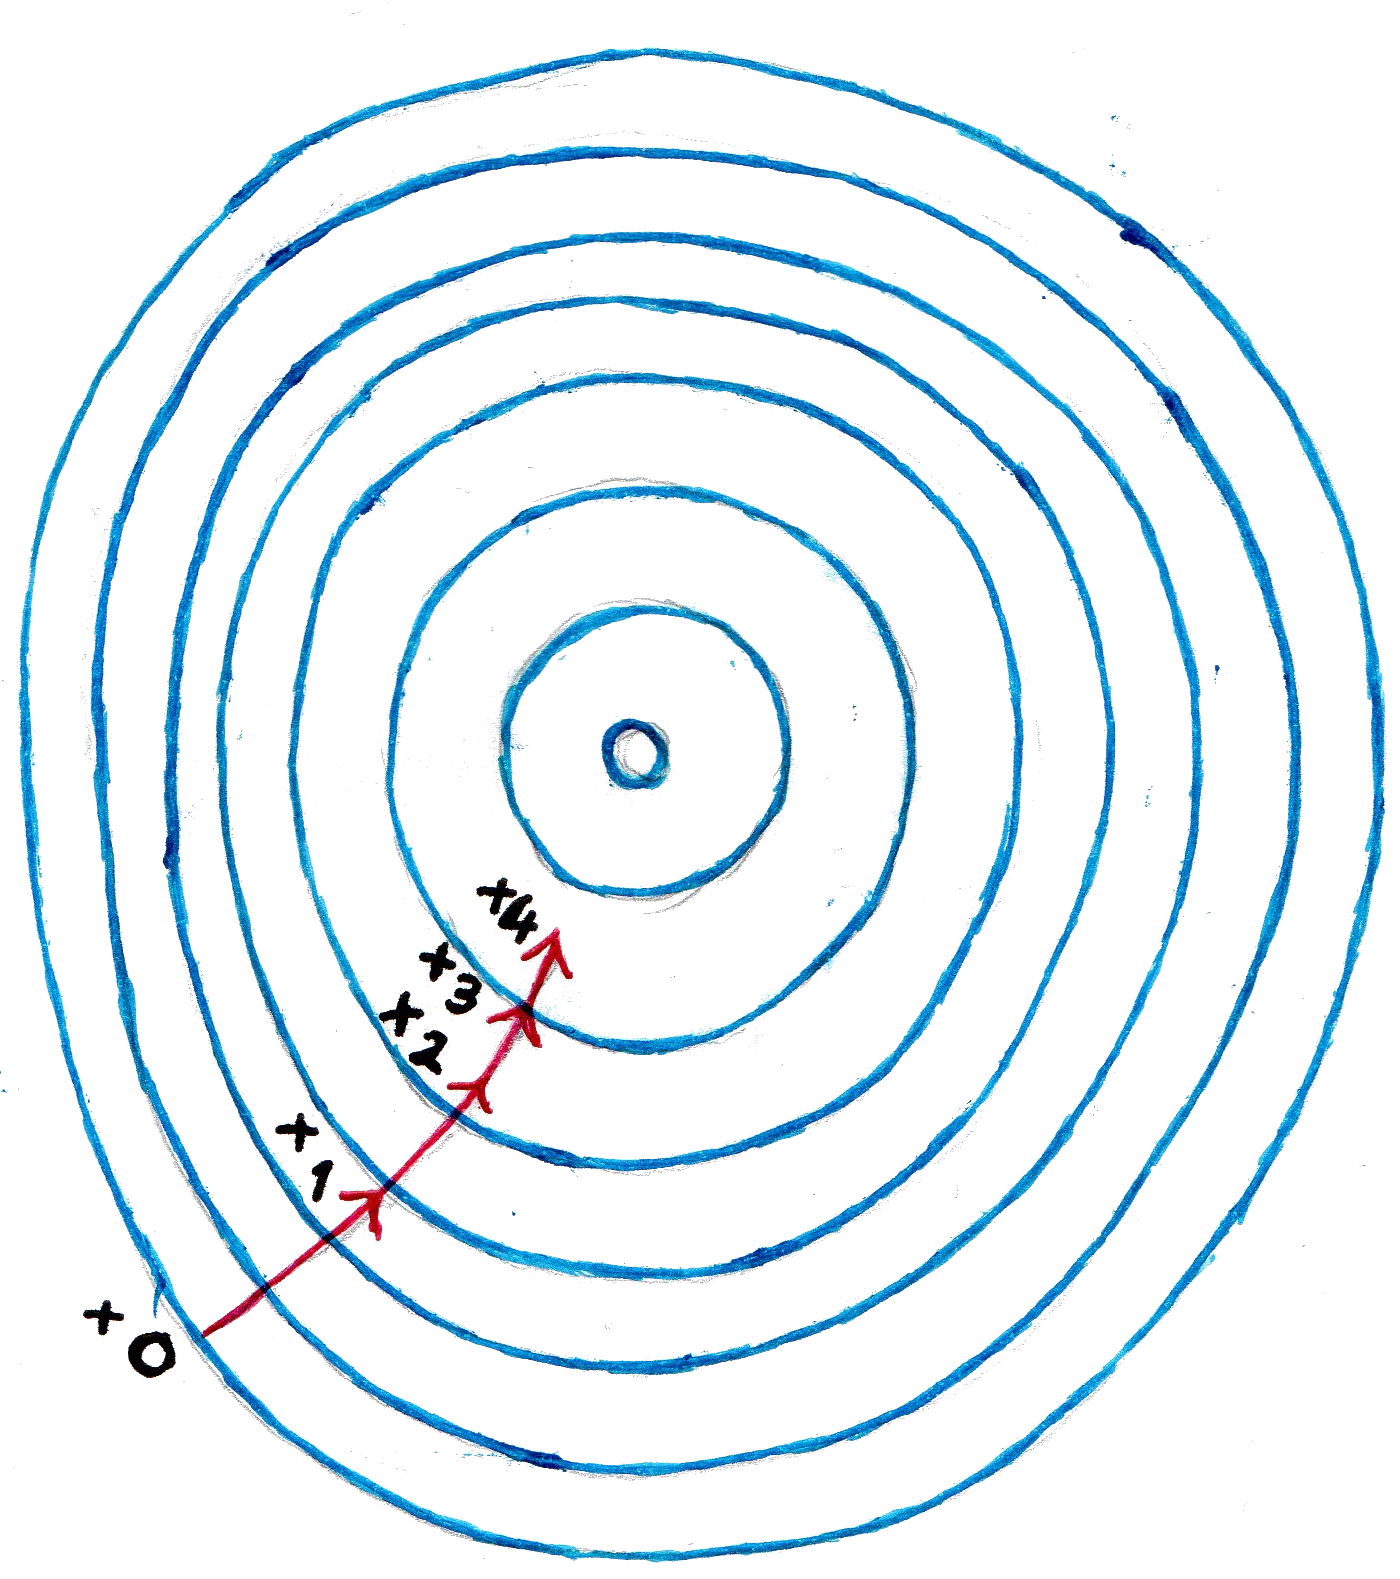
\includegraphics[width=1.0\linewidth]{figures/background_optimisation.png}
                        
                    \captionsetup{singlelinecheck=false, justification=raggedright}
                    \caption{Graphical representation of a \gls{2D} solution space and an optimiser stepping through this space. In the bottom left of this figure the initial estimate for some optimisation can be seen at $x$, the subsequent iterations $1$ through $4$ can then be seen taking this estimate closer to the centre of the contour plot. Here the contour plot could either be showing a maximisation or a minimisation depending on how it is visualised.} \label{fig:optimiser_optimisation}
                \end{figure}
                
                An optimiser takes an estimate of the solution and an objective function, as seen in~\Fref{sec:objective_function} the objective function returns the goodness of the estimate which the optimiser can either maximise or minimise. The direction in which the optimiser updates the estimate is based on the gradient of the objective function. The method by which the optimiser updates the estimate is what differentiates optimisation algorithms.
                
                \gls{GD} is a commonly used family of optimisation algorithms. \gls{GD} itself finds the gradient of the objective function at the current estimate %KT?you mean ``at the current estimate'' %ACW done
                and takes steps, of a given size,  in the direction calculated from the gradient. %which most shrinks the value of the objective function. %KT ``most'' I think is only true for ``Steepest GD''. I'd cut the 2nd half of the sentence %ACW done
                The step size of \gls{GD} can be set to a fixed value or found using a line search which optimises the step size. Momentum can be used as an improvement of \gls{GD} where the current update direction is a linear combination, with a predefined weighting, of the current gradient and the previous update direction. %KT ok, although I wouldn't call it GD anymore. I'd therefore say ``Momentum can be used as an improvement of GD'' or so %ACW done
                %Momentum attempts to reduce the effect of local minimum solutions or non-convex solution spaces by reducing the likelihood of the current update causing the optimisation to jump back and forth between two close values. %KT I disagree with tis sentence. they just try to go faster. This methods have no clue about local minima etc %ACW done
                
                \gls{SGD} is an extension of \gls{GD} where the current update is calculated using the gradients of a randomly selected subset of the data, %KT of the data (not the estimate) %ACW done
                this is significantly more computationally efficient than \gls{GD} as it reduces the number of calculations needed for each update.
                
                \gls{CG} is another extension of \gls{GD}. Here the direction of subsequent updates are confined so that they are orthogonal to the previous update direction, this can decrease convergence time~\boxcite{Tustison2009}. %KT remove the ``can avoid the same issue''. CG also attempts to go to a local minimum %ACW done
                
                \gls{BFGS} and \gls{L-BFGS} are second order optimisers in that they take the second order partial derivatives of the objective function. \gls{BFGS} and its derivatives determine the descent direction by preconditioning the gradient with curvature information. \gls{L-BFGS} is differentiated from \gls{BFGS} in that \gls{BFGS} stores a dense approximation of the inverse Hessian, whereas \gls{L-BFGS} stores a history of a past window of updates. Thus \gls{L-BFGS} uses less memory than \gls{BFGS} and thus can converge faster~\boxcite{Fletcher2000PracticalOptimization}.
                
                An optimiser can also be provided with bounds or constraints, a simple bound would be a box bound where the values of the estimate cannot exceed a threshold. \gls{L-BFGS-B} is an implementation of \gls{L-BFGS} which accepts box bounds. This can be useful, for instance, in \gls{PET} reconstruction where it is not expected that negative values should exist, so they could be constrained.
            
    \longsection{PET Image Reconstruction}{sec:pet_image_reconstruction}
        This section of the thesis follows on from the previous section in that it focuses on the inverse problem of \gls{PET} reconstructions specifically. First it shows how \gls{PET} reconstruction is an inverse problem, by likening aspects of the reconstruction problem to those presented previously, before elaborating on the two general families of reconstruction algorithm. Analytical and numerical approaches to \gls{PET} reconstruction are discussed and finally a common output scale from this process is highlighted.
            
        The second subsection expands upon the numerical approach (or optimisation) to \gls{PET} reconstruction given previously. Initially the advantages and disadvantages of iterative \gls{PET} reconstruction in general are introduced. Then common algorithms are described and their operation, advantages and disadvantages are compared. 
        
        \subsection{PET Image Reconstruction Introduction} \label{sec:analytic_image_reconstruction_introduction}
            \gls{PET} image reconstruction is an inverse problem, as stated in~\Fref{sec:inverse_problem_concepts}. This means that a \gls{PET} reconstruction algorithm takes as an argument the effects of the \gls{PET} acquisition system and attempts to determine its initial conditions, for instance the distribution of the radiotracer.
            
            There are two main families of methods through which a \gls{PET} reconstruction can be performed. First there are analytical \gls{PET} reconstruction algorithms, an analytical solution frames the problem in a better understood form and attempts to calculate the exact solution.% As stated in~\Fref{sec:analytic_image_reconstruction}.
            Secondly there are numerical solutions, for instance, iterative \gls{PET} reconstruction. Generally a numerical solution takes guesses at the solution and tests if the the problem is solved. Numerical approaches to solving inverse problems in general are discussed in~\Fref{sec:inverse_problem_concepts} and iterative \gls{PET} reconstruction algorithms are discussed in~\Fref{sec:iterative_image_reconstruction}.
            
            The data output from a \gls{PET} scan are usually expressed in \glss{KBq/mL}, however for pseudo quantitative analysis the values are usually normalised to \gls{SUV} by dividing the activity by, for instance, the mass of the patient and the injected activity. %KT previous sentence belongs in image recon section, not where you discuss the measured data %ACW done
        
%        \subsection{Analytic Image Reconstruction} \label{sec:analytic_image_reconstruction}
            % mention briefely FBP ?
            %KT no! cut. I didn't read it
            %ACW done
%            \begin{figure}
%                \centering
                    
%                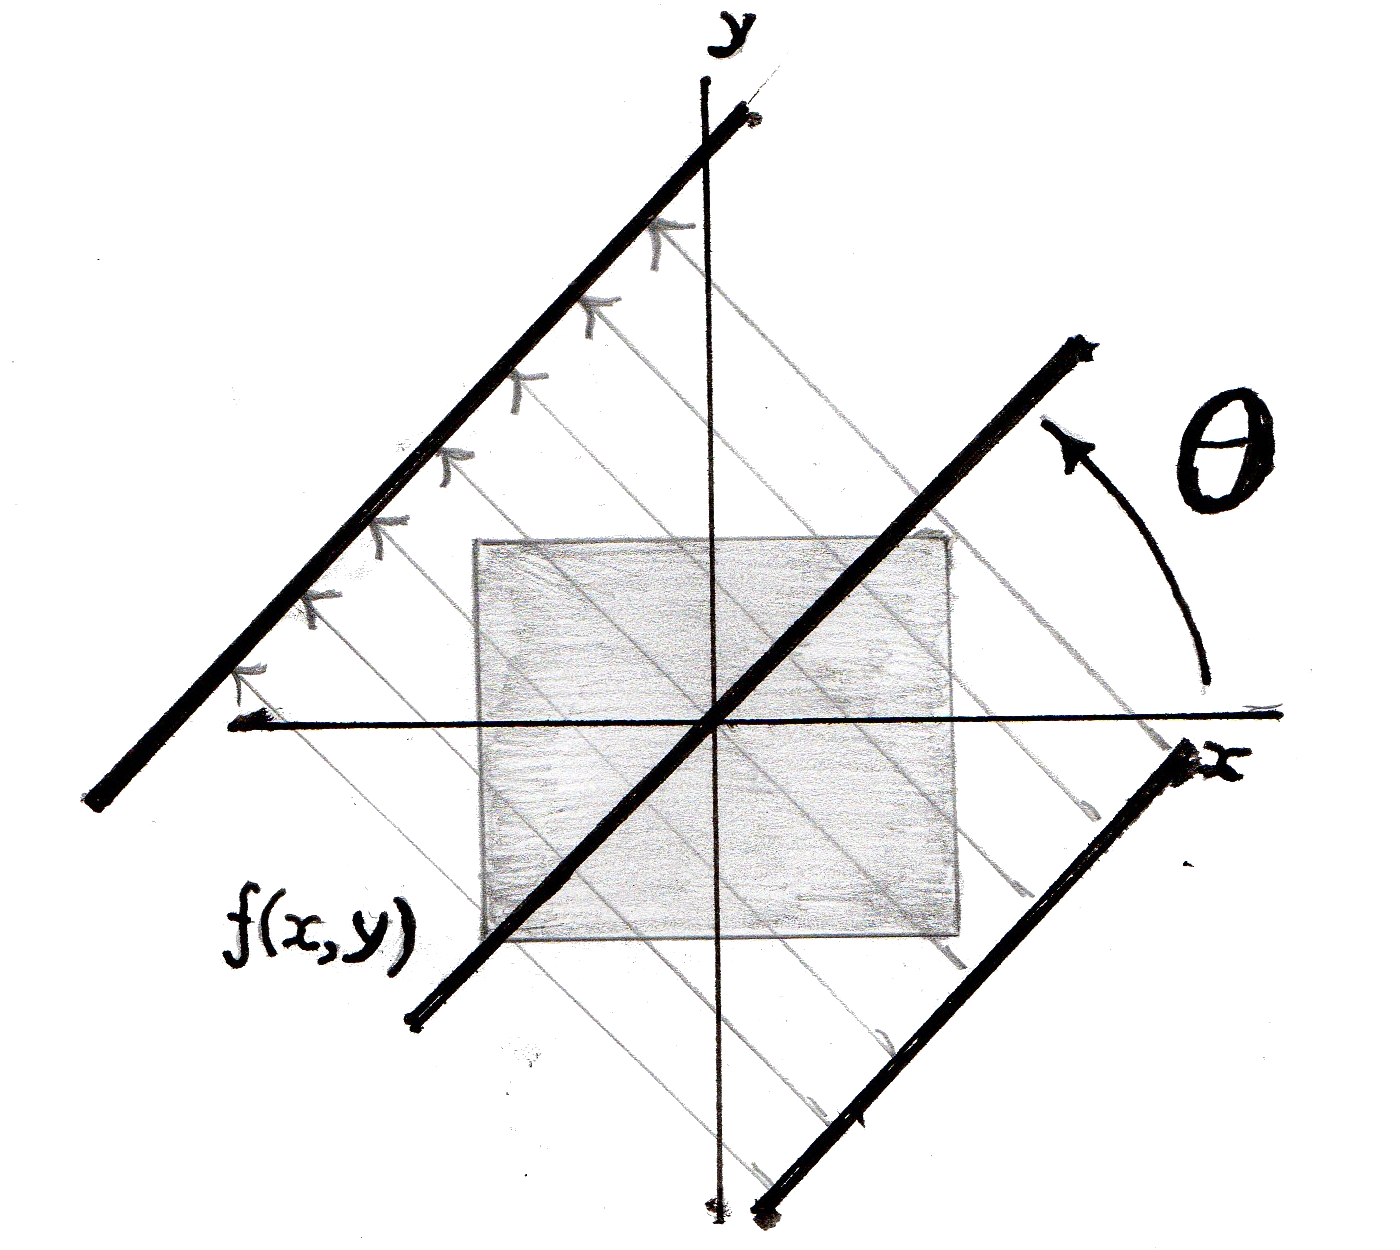
\includegraphics[width=1.0\linewidth]{figures/background_radon_transform.png}
                    
%                \captionsetup{singlelinecheck=false, justification=raggedright}
%                \caption{Graphical representation of the Radon transform for one angle $\theta$. The Radon transform computes projections of some data along specified directions. Here, this figure shows the computation of a set of line integrals for the function $f(x, y)$, usually from multiple sources of parallel beams. To form a full image the Radon transform rotates the source around the centre of the image. This figure specifically shows projections for a simple \gls{2D} image along horizontal and vertical components $x$ and $y$.} \label{fig:analytic_image_reconstruction_radon_transform}
%            \end{figure}
            
%            \begin{figure}
%                \centering
                
%                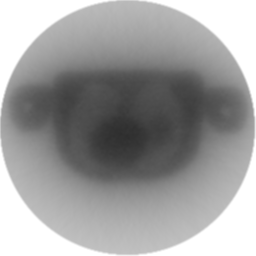
\includegraphics[width=1.0\linewidth]{figures/background_bp_example.png}
                
%                \captionsetup{singlelinecheck=false, justification=raggedright}
%                \caption{Example of a simulated \glss{AC} \gls{NTOF} \gls{BP} reconstruction, with motion and noise, with no randoms or scatters, of the thorax with a spherical lesion in the lungs. Transverse view.}
%                \label{fig:analytic_image_reconstruction_bp_example}
%            \end{figure}
            
%            \begin{figure}
%                \centering
                
%                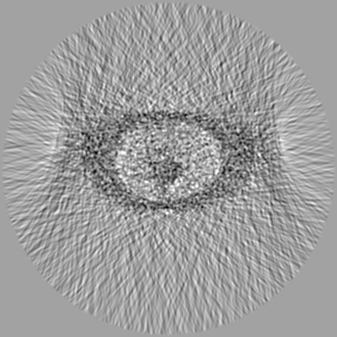
\includegraphics[width=1.0\linewidth]{figures/background_fbp_example.png}
                
%                \captionsetup{singlelinecheck=false, justification=raggedright}
%                \caption{Example of a simulated \glss{AC} \gls{NTOF} \gls{FBP} reconstruction, with motion and noise, with no randoms or scatters, of the thorax with a spherical lesion in the lungs. Transverse view.}
%                \label{fig:analytic_image_reconstruction_fbp_example}
%            \end{figure}
            
%            An analytic solution is one which offers a direct mathematical method through which one thing can be transformed to another. All analytical solutions can have a proof. An analytical solution for \gls{PET} reconstruction is \gls{BP}, in \gls{2D} \gls{BP} is the inverse Radon transform. This can be seen in~\Fref{fig:analytic_image_reconstruction_radon_transform}. To apply the inverse Radon transform to a \gls{2D} sinogram; first the rows of the sinogram, corresponding to $\SI{0}{^{\circ}}$ through $\SI{180}{^{\circ}}$, are taken individually and have the Fourier transform applied to them. Then the result of this is reshaped to polar coordinates so that each row is the diameter of a circle and a \gls{2D} Fourier transform is applied giving the final output image. The Fourier transform decomposes a function into its constituent frequencies. The \gls{2D} Fourier transform of a function computed along a line is equivalent to the 1D Fourier transform of the Radon transform along that line. This is called projection slice theorem. 
            
%            \gls{FBP} was proposed as a solution to some of the issues apparent in \gls{BP}, like the fact that \gls{BP} suffers from low frequency blurring. In \gls{FBP} a high pass ramp filter is applied to the sinogram before it is Fourier transformed, thus removing some low frequency information or blurring. A low pass ramp filter can also be applied at the same time which removes some high frequency information or noise, this then would be a band pass filter. An example of a \gls{BP} and \gls{FBP} reconstruction can be seen in~\Fref{fig:analytic_image_reconstruction_bp_example} and~\Fref{fig:analytic_image_reconstruction_fbp_example}. Because of its speed and good quantitative results \gls{FBP} was the gold standard of \gls{PET} \gls{IR}, however because of the issues mentions above it has now almost entirely been replaced by iterative reconstruction methods. \gls{FBP} is now almost solely used in longitudinal studies which started before the use of iterative reconstruction methods became prevalent~\boxcite{FBPReviewBib}~\boxcite{PETCTReviewBib}.
            
%            \gls{BP} and \gls{FBP} reconstruct a low quality image but are computationally fast. \gls{BP} will usually result in there being numerous streak like artefacts in the output image, the artefacts are exacerbated as noise increases. Artefacts can be caused because neither \gls{BP} nor \gls{FBP} account for the stochastic nature of the acquisition process, neither do they account for other factors such as positron range as discussed in~\Fref{sec:attenuation}.
            
            
        \subsection{Iterative Image Reconstruction} \label{sec:iterative_image_reconstruction}
            \begin{figure}
                \centering
                
                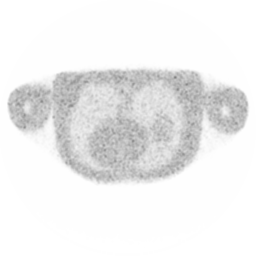
\includegraphics[width=1.0\linewidth]{figures/background_osem_example.png}
                
                \captionsetup{singlelinecheck=false, justification=raggedright}
                \caption{Example of a simulated \gls{AC} \gls{NTOF} \gls{OSEM} reconstruction, with motion and noise, with no randoms or scatters, of the thorax with a spherical lesion in the lungs. Transverse view.}
                \label{fig:iterative_image_reconstruction_osem_example}
            \end{figure}
            
            %As discussed above in~\Fref{sec:inverse_problems_and_optimisation} an inverse problem, which \gls{PET} reconstruction is, can be solved by an iterative optimisation problem. In order to implement an iterative optimisation problem a few criteria must first be met; a forward operator which takes an image and return the projections which would result from acquiring the image is required. As discussed above in~\Fref{sec:optimisation_concepts} an objective function to assess the accuracy of the fit and an optimisation algorithm to improve the fit are required. Also, an initial estimate, which could be a volume the size of the output image filled with ones or zeros, and some method to cease execution, for instance stopping when the objective function reaches a certain value or the number of iterations exceeds a threshold, are also necessary. %KT cut all this here as strong overlap with previous section. Move statement about initial estimate and stopping criteria there. %ACW done

            %KT cut some stuff if cutting analytic recons above
            An iterative method has the advantage that the model which is used can take into account the noise properties of the data and also the physical properties of the scanner. The noise associated with \gls{PET} is often assumed to be Poisson distributed. However, iterative methods have the disadvantage that, because they are significantly complex, they require substantial computational effort to execute, this will increase computation time when compared to analytical reconstruction.
            
            %\gls{ML} is a commonly used objective function for iterative \gls{PET} reconstruction. This builds on the concepts, specifically \gls{MLE}, mentioned in~\Fref{sec:objective_function}. %KT cut previous sentence. no need to repeat all the time %ACW done
            \gls{ML} is often combined with the \gls{EM} algorithm for the optimisation of the model parameters and in this case is called \gls{MLEM}~\boxcite{MLEMBib}~\boxcite{PETMLEMBib}~\boxcite{PETMLEM2Bib}. When maximising the likelihood the natural logarithm of the likelihood, also known as the log-likelihood, is taken for computational efficiency. The output from \gls{MLEM} commonly has a Gaussian blur applied in order to smooth noise~\boxcite{PETMLEMFiltBib}. Disadvantages associated with \gls{MLEM} include, for noisy data iterating for too long can cause the output to accentuate the noise present in the data, one way to avoid this is to purposefully cease iterating early before the noise can take over the image~\boxcite{PETMLEMTerminationBib}. Another issue is that \gls{MLEM} is exceptionally slow even when compared to other iterative algorithms. %KT ``as mentioned earlier, as will be discussed below''. only the latter I guess %ACW done
            
            To combat the slow execution speed of \gls{MLEM} \gls{OSEM} was developed. In \gls{OSEM} the \gls{LOR} or detector pairs of the scanner are binned into a number of subsets. This is in contrast to \gls{MLEM} where there is logically one subset, \gls{MLEM} would be applied to all \gls{LOR} or detector pairs simultaneously. However, in \gls{OSEM} the \gls{LOR} or detector pairs could be binned into at least two subsets. \gls{MLEM} is then applied to each subset, in a specific order, sequentially~\boxcite{OrderedSubsetsHudsonBib}~\boxcite{OrderedSubsetsHuttonBib}. Because the image is updated after each iteration of \gls{MLEM} on each subset of \gls{OSEM} then the execution speed of \gls{OSEM} is increased by the number of subsets used. However, if% more than two 
            subsets are used %KT even with 2 actually... %ACW done
            then  \gls{OSEM} will converge to a limit cycle around true convergence~\boxcite{Mettivier2011}. If a reasonable number of subsets are used it has been found that \gls{OSEM} will accelerate \gls{MLEM} without affecting the accuracy of quantification too drastically~\boxcite{Morey2013}. An example of an \gls{OSEM} reconstructed image can be seen in~\Fref{fig:iterative_image_reconstruction_osem_example}.
            
    \longsection{Respiratory Motion in PET}{sec:respiratory_motion_in_pet}
        % general intro
        This section of the thesis introduces the problem of \gls{RM} in \gls{PET}/\gls{CT}. First it addresses how \gls{RM} presents specifically in reconstructed \gls{PET} volumes and what this can mean for clinical diagnosis. Next the issue of \gls{RM} in combined \gls{PET}/\gls{CT} is highlighted and the challenges associated with the misalignment of the data between modalities is touched on, including how this could negatively impact the \gls{AC} reconstructed \gls{PET} volume (issues introduced by the \gls{PET}/\gls{CT} workflow in the clinic are also presented).
            
        The second subsection expands upon the challenges introduced by \gls{RM} in the combined \gls{PET}/\gls{CT} workflow and lists some methods from the clinic and the literature which have been developed to combat this.
        
        \subsection{Respiratory Motion Artefacts} \label{sec:respiratory_motion_artefacts}
            % have a look at https://www.sciencedirect.com/science/article/pii/S0001299808000214?via%3Dihub
            
            \begin{figure}
                \centering
                
                
\includegraphics[width=1.0\linewidth]{figures/background_motion_artefact_example.png}
                
                \captionsetup{singlelinecheck=false, justification=raggedright}
                \caption{Example of a simulated \gls{AC} \gls{NTOF} \gls{OSEM} reconstruction, with motion, with no noise, randoms or scatters, of the thorax with a spherical lesion in the lungs. Coronal view.}
                \label{fig:respiratory_motion_artefacts_motion_artefact}
            \end{figure}
            
            \begin{figure}
                \centering
                
                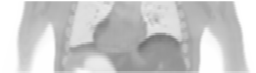
\includegraphics[width=1.0\linewidth]{figures/background_single_mu-map_ac_example.png}
                
                \captionsetup{singlelinecheck=false, justification=raggedright}
                \caption{Example of a simulated single \gls{Mu-Map} \gls{AC} \gls{NTOF} \gls{OSEM} reconstruction, with motion, with no noise, randoms or scatters, of the thorax with a spherical lesion in the lungs. Coronal view.}
                \label{fig:respiratory_motion_artefacts_single_mu-map_ac}
            \end{figure}
            
            A static single bed position acquisition on a conventional \gls{PET} scanner takes, on average, approximately \SI{120}{\second}. This means that, because the patient is in \gls{RM} throughout the acquisition, then the result of the scan will contain data from different respiratory states. During the different respiratory states the position and volume of the lungs, diaphragm and any lesion will change. If the data is reconstructed without accounting for this then there will be the presence of blurring artefacts (especially prevalent around the anatomy that is moving the most, such as the diaphragm). %This would be expected as the data, in this case, represents as if the respiratory states had been summed together. %KT let's cut the previous sentence in an attempt to be less verbose :-) %ACW done
            An example of a \gls{PET} reconstruction with motion artefacts can be seen in~\Fref{fig:respiratory_motion_artefacts_motion_artefact}, notice the blurring above the diaphragm on the right side of the figure. Artefacts originating from the moving anatomy pose the largest challenge in imaging of the thorax~\boxcite{LungMotionArtefactBib}~\boxcite{PETCTArtifactBib}.
            
            The artefacts caused by \gls{RM} lead to issues clinically with cancer staging and follow up. This is because the size of the tumour is often overestimated and the activity underestimated (the activity in the lesion is spread over more voxels) thus it has the capacity to cause lesions to potentially be missed due to reduced detectability~\boxcite{LungMotionJudgmentErrorsBib}. %KT and lesions potentially to be missed (i.e reduced detectability) %ACW done
            
            If \gls{AC} is used then the position of the \gls{Mu-Map} in relation to the \gls{PET} data also poses an issue. Where the \gls{Mu-Map} does not match the position of the anatomy then it will cause either under or over-correction of the attenuation. This can cause a type of artefact often referred to as a banana artefact due to the shape of the shadow that it causes to appear above the diaphragm~\boxcite{LungMotionDiaphragmBaiBib}. An example of this can be seen in~\Fref{fig:respiratory_motion_artefacts_single_mu-map_ac}. Notice the black arc shaped artefact over the diaphragm and on the heart. The mismatch of the \gls{Mu-Map} and \gls{PET} data does not just cause this artefact but it can also change the expectation and thus the quantification of the reconstructed image. To combat intra-\gls{Mu-Map} motion the patient will often be asked to hold their breath, if they can, as the \gls{CT} acquisition can last for only between \SI{2.0}{\second} and \SI{3.0}{\second}~\boxcite{Nyflot}. An issue with this is, that often the breath hold \gls{CT} will be taken at full inspiration, if this \gls{Mu-Map} is then used to correct for attenuation in data that is in a respiratory phase other than full inspiration then a lot of this anatomy will have been moved into the \gls{FOV} (it is not present in the \gls{Mu-Map}). Furthermore, when a patient is asked to hold their breath they often inhale deeper than they otherwise would, meaning that this \gls{Mu-Map} can be in an unrealistic respiratory state that will not be represented in the \gls{PET} data taken during free breathing. %KT this last sentence is incorrect. ``intra-mu-map'' motion can indeed by circumvented lrgely by breathold (as it's a CT). however, most people would do this at full inspiration, and then you get into serious trouble. %ACW done
            
        \subsection{Respiratory Motion Challenges in Combined PET/CT Imaging} \label{sec:respiratory_motion_challenges_in_combined_pet_ct_imaging}
            To overcome the issues mentioned in~\Fref{sec:respiratory_motion_artefacts}, specifically related to the mismatch between \gls{Mu-Map} and \gls{PET} data a number of solutions have been proposed:
            
            \begin{itemize}
                \item Firstly, a method which acquires \gls{PET} data over a prolonged acquisition and throws away any data where the patient is in a position other than the one that corresponds most closely to the breath hold \gls{CT} \gls{Mu-Map}. For this all data which is not at full inspiration would be removed~\boxcite{Liu2010}~\boxcite{Grootjans2014}. %KT I'd rather say that the CT is then at breathhold first. %ACW done
                The breath hold \gls{CT} \gls{Mu-Map} could then be warped to this data~\boxcite{LungMotionBreathHoldBib}. An advantage of this approach is that it would not only correct for the misalignment of \gls{Mu-Map} and \gls{PET} data but it could also eradicate most blurring associated with averaging over respiratory phases. A disadvantage is that, either there would be substantially more noise in the reconstructed data (if the acquisition was the same length as a standard one) or the acquisition could take significantly longer (to acquire an equivalent number of counts), as so much data is being removed~\boxcite{Nehmeh2008a}. Additionally, dynamic scans would not be possible with this correction method. This is because the tracer kinetics could be shorter than one respiratory cycle and thus would be lost when those parts of the acquisition are removed.
                
                \item Secondly, a variation of the previous method has been proposed, where the \gls{PET} data is separated into individual images representing the separate respiratory phases and warped to a common respiratory phase (seen in~\Fref{sec:image_registration}). The breath hold \gls{CT} \gls{Mu-Map} could then be warped to the same common respiratory phase. This method provides the advantage over the first in that it uses all of the data from the \gls{PET} acquisition and provides a more robust reconstruction~\boxcite{4DPhaseMatchedReconBib}. A disadvantage is, that the reconstruction of each respiratory phase is likely to contain more noise than if all of the \gls{PET} data was reconstructed simultaneously. This is because the iterative reconstruction algorithm (seen in~\Fref{sec:iterative_image_reconstruction}) is non-linear (analytical reconstructions are linear but are not used clinical anymore) and summing reconstructed volumes is not equivalent to summing projection data, reconstructing and then summing again. %KT true, but you then first need to say that the images are summed again. %ACW done
                In addition, the higher levels of noise in the reconstructed data can pose a problem when attempting to warp the \gls{Mu-Map} to them.
                
                \item Finally, a method where the reconstruction and motion parameters can be estimated simultaneously, directly from the \gls{PET} data, for one breath hold \gls{CT} \gls{Mu-Map} has been recently proposed~\boxcite{JacobsonFesslerMotionCorrectionBib}~\boxcite{Rezaei2012}~\boxcite{Bousse2016a}. Here, the \gls{PET} data is split into the respiratory phases, as above. Then the method iterates between a reconstruction step (seen in~\Fref{sec:iterative_image_reconstruction}) and a motion parameter estimation step (seen in~\Fref{sec:image_registration}) where the same parameters are used to warp both the \gls{PET} data and the \gls{Mu-Map} for each respiratory position. Thus the \gls{Mu-Map} does not have to correspond to any one respiratory phase as each set of \gls{PET} data will be reconstructed at the position of the \gls{Mu-Map}. This method works especially well when \gls{TOF} data is available~\boxcite{Bousse2016b}. A disadvantage of this method is that it takes more computation than the above methods and that it has not been as extensively evaluated.
            \end{itemize}
    
    \longsection{Motion Correction for PET}{sec:motion_correction_for_pet}
        This section of the thesis concerns all things \gls{MC} (specifically when applied to \gls{PET}). The first subsection introduces the concept of \gls{IR}, initially highlighting its similarity to \gls{PET} reconstruction (in the sense that they are both optimisation problems) before moving on to discussing the classification of motion types and how they can be corrected. The first kinds of deformation, briefly mentioned, are \gls{RD} and \gls{AD} then \glss{NRD} are introduced and classic approaches to alleviating them are highlighted, including parametric and nonparametric registration and methods of regularising them are touched on.
        
        The second subsection moves on to introduce the concept of respiratory gating, including both amplitude and phase gating before the third subsection which explains how the \glss{SS}, which are used in respiratory gating, are acquired. Firstly methods incorporating external devices to extract \glss{SS} are highlighted, including using the \gls{RPM}, then moving onto \gls{DD} methods. \gls{PCA} is explained as a dimensionality reduction technique and its use for acquiring \glss{SS} directly from \gls{PET} acquisition data is provided.
        
        The fourth subsection gives examples of how to combined \gls{IR} and respiratory gating, specifically mentioning pairwise and groupwise registration before an extension of vanilla \gls{IR} is introduced in the fifth subsection. Here \gls{MM}, both iteratively and simultaneously with \gls{IR} is introduced including simple \gls{MM} (for instance, a linear regression of \glss{DVF} and \gls{SS}) as well as more complex \gls{MM} approaches. Furthermore, different types of \gls{RCM} and their formation, advantages and disadvantages are touched on.
        
        The final subsection is related to the actual application of \gls{MC}, for instance, how and where it is applied. This includes highlighting the benefits of both a post reconstruction and iterative with reconstruction schema.
    
        \subsection{Image Registration} \label{sec:image_registration}
            \gls{IR} is an optimisation problem which attempts to warp one image (called the dynamic image) to another image (called the static image). The way that one image is warped to another image is through the use of a transformation (or \gls{DVF}). There are  different kinds of deformations including \glss{RD} and \glss{NRD} which will be discussed in the following sections in~\Fref{sec:rigid_deformation} and~\Fref{sec:non_rigid_deformation} respectively. These deformations directly deform or warp the dynamic image so that it best matches the static image. %If there are multiple dynamic images then the optimisation will produce a transformation for each image.
            The images used for \gls{IR} do not necessarily need to be from the same modality and as such \gls{CT} data can be registered to \gls{PET} data or vice versa. A common use for \gls{IR} in medical imaging is to aid in the process of \gls{MC}.
            
            As discussed in~\Fref{sec:optimisation_concepts} an optimisation requires an objective function. In the case of \gls{IR} the most common objective functions are \gls{MSE}, \gls{CC} and \gls{MI}. \gls{MSE} is discussed in~\Fref{sec:objective_function} but simply assumes that once the dynamic image has been deformed to the static then the images should be identical, thus \gls{MSE} is best used when the only difference between the two images is from, for instance, motion and not from a change in modality. \gls{CC} and \gls{MI} are less reliant on the specific intensity values of an image and instead look for relationships between intensities, thus they are more suitable to registering between different modalities than \gls{MSE}~\boxcite{Hill2001}~\boxcite{Oliveira2014}.
            
            One difference between the optimisation for \gls{PET} reconstruction and for \gls{IR} is that the stochastic nature of the data is not usually taken into account in the model for \gls{IR}.
            
            \subsubsection{Rigid Deformation} \label{sec:rigid_deformation}
                \begin{figure}
                    \centering
                    
                    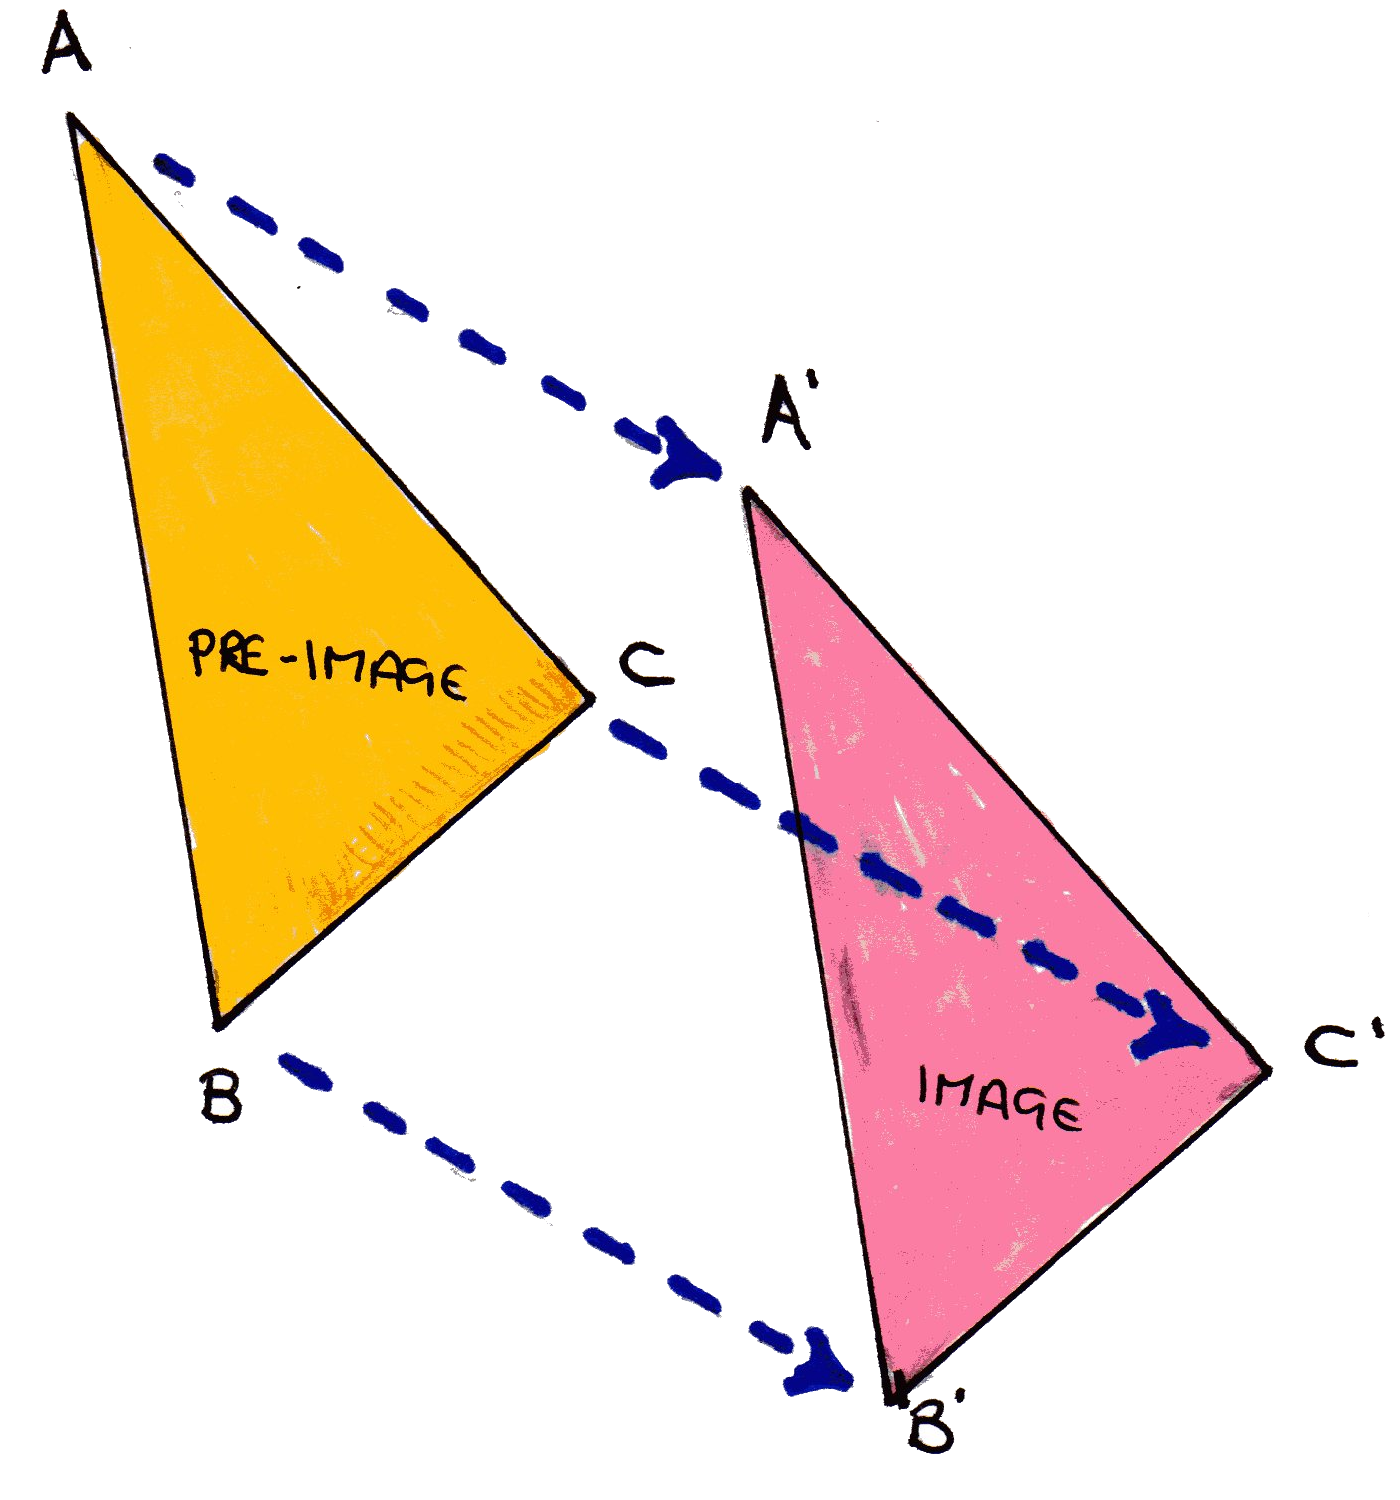
\includegraphics[width=1.0\linewidth]{figures/background_rd.png}
                    
                    \captionsetup{singlelinecheck=false, justification=raggedright}
                    \caption{Graphical representation of a \gls{RD}. On the left a triangle with vertices $A$, $B$ and $C$ can be seen, this triangle undergoes a \gls{RD} (a translation down and to the right) to a triangle, on the right, with vertices $A'$, $B'$ and $C'$.} \label{fig:rigid_transformations_rd}
                \end{figure}
                
                \begin{figure}
                    \centering
                    
                    \includegraphics[width=0.9\linewidth]{figures/background_ad.png}
                    
                    \captionsetup{singlelinecheck=false, justification=raggedright}
                    \caption{Graphical representation of an \gls{AD}. In the centre a cyan leaf can be seen which undergoes an \gls{AD} (a translation down and to the left, a rotation anticlockwise and a scale down) to a red leaf, on the left. The cyan leaf also undergoes an \gls{AD} (a translation down and to the right, a rotation clockwise, a scale down and a skew) to a blue lead, on the right.} \label{fig:rigid_transformations_ad}
                \end{figure}
                
                A \gls{RD} could be a rotation or a translation of the entire contents of an image where the same rotation or translation is applied at every point. A \gls{RD} is one where the euclidean distance between every pair of points in the image is consistent before and after the deformation is applied, this can be seen in~\Fref{fig:rigid_transformations_rd}. \glss{RD} are a subset of a type of deformation called an \gls{AD}. A \gls{3D} \gls{RD} has six degrees of freedom, being rotation and translation in every axis, whereas a \gls{3D} \gls{AD} has $12$ degrees of freedom, rotation, translation, scaling and sheering in every axis. An \gls{AD} does not guarantee that the euclidean distance between pairs of points are maintained, this can be seen in~\Fref{fig:rigid_transformations_ad}.
                
                \glss{RD} are often used in medical imaging where the anatomy which is being registered is not expected to undergo individual internal motion, for instance \glss{RD} are often used in the registration of patient head motion~\boxcite{Hill2001}. \glss{AD} are not often used in medical imaging as anatomy does not usually deform in ways that \glss{AD} can capture but \glss{RD} cannot, although an \gls{AD} can be used as an initial estimate for fitting a more complex \gls{NRD}.
                
                The output from a \gls{RD} or \gls{AD} is usually the values from the six or $12$ value transformation matrix, respectively, and as such they do not take up much computational memory or storage.
                
            \subsubsection{Non-Rigid Deformation} \label{sec:non_rigid_deformation}
                \begin{figure}
                    \centering
                    
                    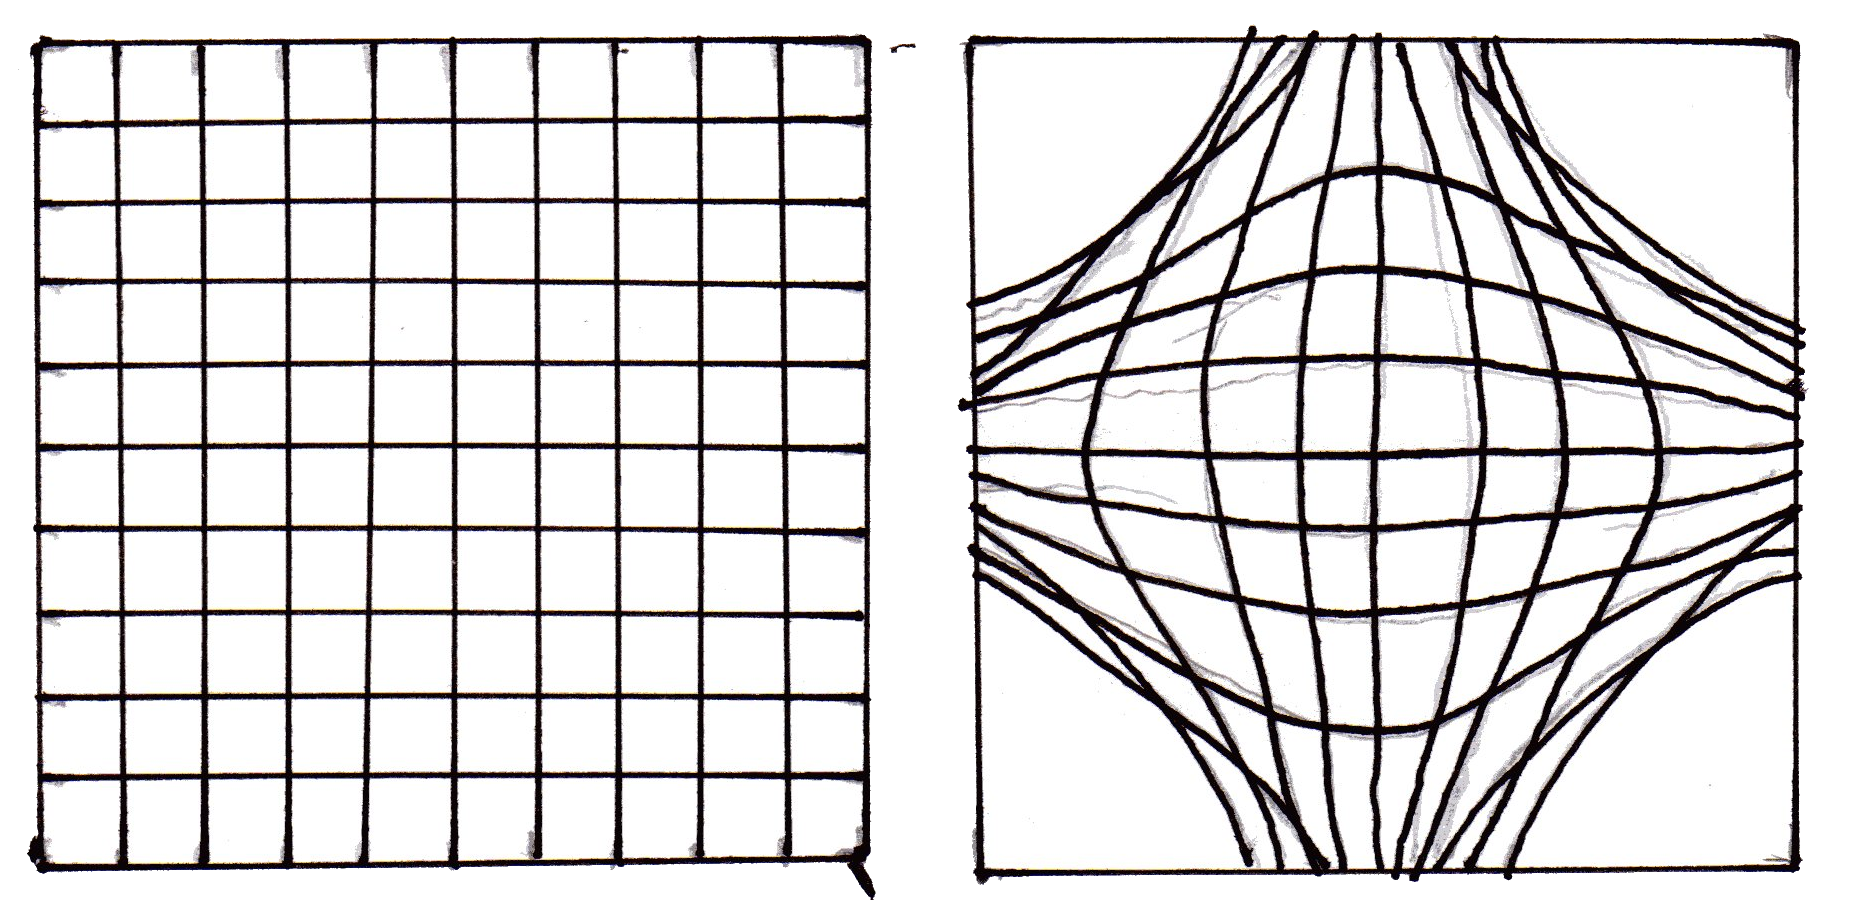
\includegraphics[width=1.0\linewidth]{figures/background_nrd.png}
                    
                    \captionsetup{singlelinecheck=false, justification=raggedright}
                    \caption{Graphical representation of a \gls{NRD}. On the left a grid can be seen, this grid undergoes a \gls{NRD} to the grid on the right.} \label{fig:non_rigid_deformation_nrd}
                \end{figure}
                
                A \gls{NRD} is one where the euclidean distance between pairs of points is not maintained, this can be seen in~\Fref{fig:non_rigid_deformation_nrd}. Notice that the euclidean distance between where the lines of the grids intersects changes between the grid on the left and the grid on the right. %For example the motion of a fluid is a \gls{NRD} as pairs of points can move past each other by different amounts.
                \glss{NRD} are commonly seen in medical imaging in \gls{RM} as the diaphragm and lungs experience sliding motion and displace different parts of the patient's anatomy by different amounts over the respiratory cycle. A \gls{NRD} is often represented by a \gls{DVF} which is, in the simplest case, a volume (the same size, with the same number of elements, as the data) where each 'voxel' contains a vector that points either from the voxel in the dynamic image to the same voxel (anatomically, not literally) in the static image or vice versa.
                
                However, for reasons of computational efficiency (and usually to regularise the \gls{IR} optimisation, somewhat) the \gls{DVF} can be parameterised. One parameterisation could be to use \glss{CP} on a \gls{CPG} which are interpolated using, for instance, linear or \gls{BS} interpolation to find the vector to be applied at each voxel~\boxcite{Bardinet1996}~\boxcite{Rueckert1999}~\boxcite{Mattes2003}~\boxcite{JacobsonFesslerMotionCorrectionBib}. There are also \gls{IR} methods which forego parameterisation and instead directly fit the \gls{DVF}, for instance Daemon registration (also known as nonparametric registration algorithms)~\boxcite{VercauterenDiffeomorphicRegistration}.
                
                Regularisation terms are often employed for \glss{NRD} \gls{IR} as otherwise with a high resolution \gls{CPG} it is possible for the optimisation to fit the noise present in the data rather than fitting the motion, as discussed in~\Fref{sec:optimisation_concepts}. One common form of regularisation is a smoothness penalty, for instance \gls{TPS}, \gls{BE} or \gls{LE}. Here, simply, the term is calculated as the integral of the square of the second derivative of the \gls{DVF}. This term is multiplied by some value $\epsilon$ representing the weighting of this penalty term and then the scaled term is summed to the current value of the objective function. This regularisation term attempts to enforce that adjacent \glss{CP} should not rapidly change, with regards to one another, as this type of motion is unlikely physically~\boxcite{Duchon1977SplinesSpaces}. In the case of nonparametric registration, a Gaussian smoothing of the input data is sometimes used for regularisation~\boxcite{VercauterenDiffeomorphicRegistration}.
        
        \subsection{Respiratory Gating} \label{sec:respiratory_gating}
            % brief intro
            
            \begin{figure}
                \centering
                    
                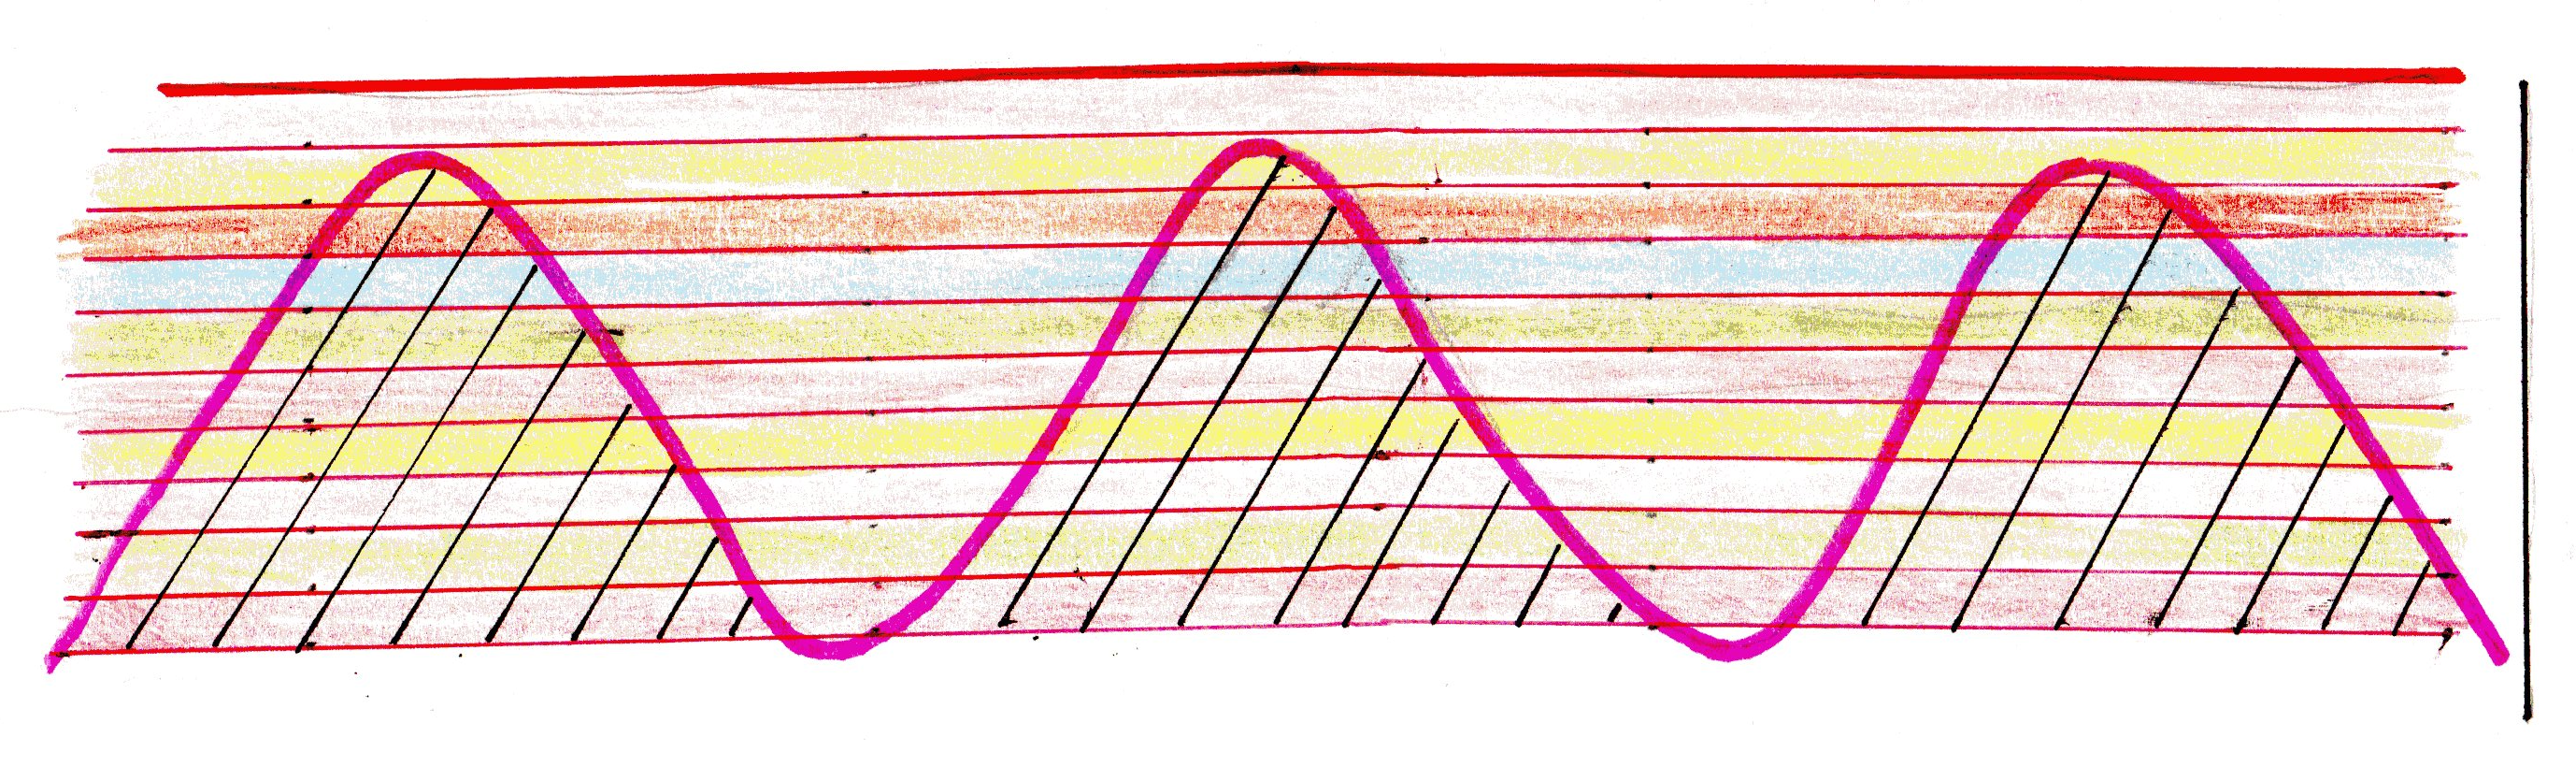
\includegraphics[width=1.0\linewidth]{figures/background_amplitude_gating.png}
                    
                \captionsetup{singlelinecheck=false, justification=raggedright}
                \caption{Graphical representation of amplitude gating. Here the red pseudo sinusoidal signal represents the \gls{SS} and the horizontal lines, colour coded differently, represent the amplitude gates that the data upon the \gls{SS} would be binned into.} \label{fig:respiratory_gating_ampliude_gating}
            \end{figure}
            
            \begin{figure}
                \centering
                    
                \includegraphics[width=1.0\linewidth]{figures/background_full_phase_gating.png}
                    
                \captionsetup{singlelinecheck=false, justification=raggedright}
                \caption{Graphical representation of phase gating. Here the red pseudo sinusoidal signal represents the \gls{SS} and the vertical lines, colour coded differently, represent the phase gates that the data upon the \gls{SS} would be binned into.} \label{fig:respiratory_gating_full_phase_gating}
            \end{figure}
            
            The method of respiratory gating was briefly touched on previously in~\Fref{sec:respiratory_motion_challenges_in_combined_pet_ct_imaging}. Here the process of specifically how respiratory gating works will be addressed. In order to separate \gls{PET} acquisition data (so that counts only in a certain window or respiratory phase are combined into specific gates or bins), a \gls{SS} which reflects the respiratory state of the patient, over time, must be acquired. This \gls{SS} can either directly reflect the amplitude of the patient's breathing or can be a percentage of the phase through which the patient is in the respiratory cycle, at any one time~\boxcite{Kitamura2017TheMethods.}. These two types of \glss{SS} directly influence the type of gating that will be performed, these two types are:
            
            \begin{itemize}
                \item Firstly, amplitude gating takes the maximum and minimum value of the \gls{SS} and splits the values between them into a number of gates, this can be seen in~\Fref{fig:respiratory_gating_ampliude_gating}. The gates can be chosen so that they are either equally spaced apart or so that each gate has a similar number of counts binned into them. The acquisition data is gated by taking its relevant \gls{SS} value and summing it in into the bin where it falls between the maximum and minimum threshold of the bin.
                
                \item Secondly, phase gating works exactly the same as amplitude gating but rather than splitting the data up along the \gls{SS} it can be conceptualised as splitting the data up temporally by the phase of the respiratory cycle, this can be seen in~\Fref{fig:respiratory_gating_full_phase_gating}.
            \end{itemize}
            
            Both types of respiratory gating can be augmented by incorporating other signals. For instance, amplitude gating can bin data into gates for both the inspiration and expiration parts of the respiratory cycle by also gating over the gradient of the \gls{SS}~\boxcite{Low2005}.
        
        \subsection{Respiratory Signal Detection} \label{sec:respiratory_signal_detection}
            As mentioned in~\Fref{sec:respiratory_gating} it is necessary to acquire a signal which represents the position in the respiratory cycle that the patient is in, over the acquisition, not only for respiratory gating but also for \gls{MM} (as will be discussed in~\Fref{sec:motion_modelling}). There are two types of methods through which a \glss{SS} can be obtained. These are from an external mechanical or electrical devices (which directly physically measure the patient) or through \gls{DD} algorithms which attempt to extract the \gls{SS} from the data of the acquisition itself.
            
            \subsubsection{External Devices} \label{sec:external_devices}
                \begin{figure}
                    \centering
                        
                    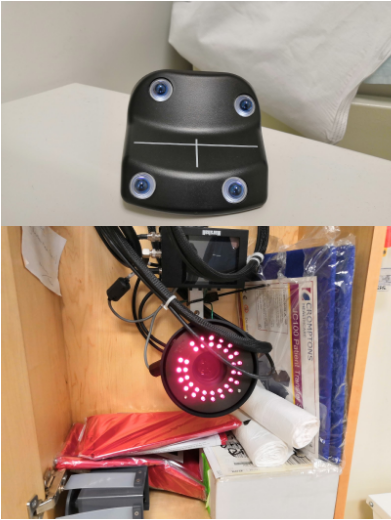
\includegraphics[width=1.0\linewidth]{figures/background_rpm.png}
                        
                    \captionsetup{singlelinecheck=false, justification=raggedright}
                    \caption{Photograph of the \gls{RPM}. On the bottom is the infrared camera and infrared \glss{LED} used to locate and track an infrared reflecting marker. On the top is the infrared reflecting marker which is placed onto the chest or stomach of the patient in order to track the respiratory amplitude of the patient. Four reflective points are used to track the marker in \gls{3D} plus a point for redundancy.} \label{fig:external_devices_rpm}
                \end{figure}
                
                \begin{figure}
                    \centering
                    
                    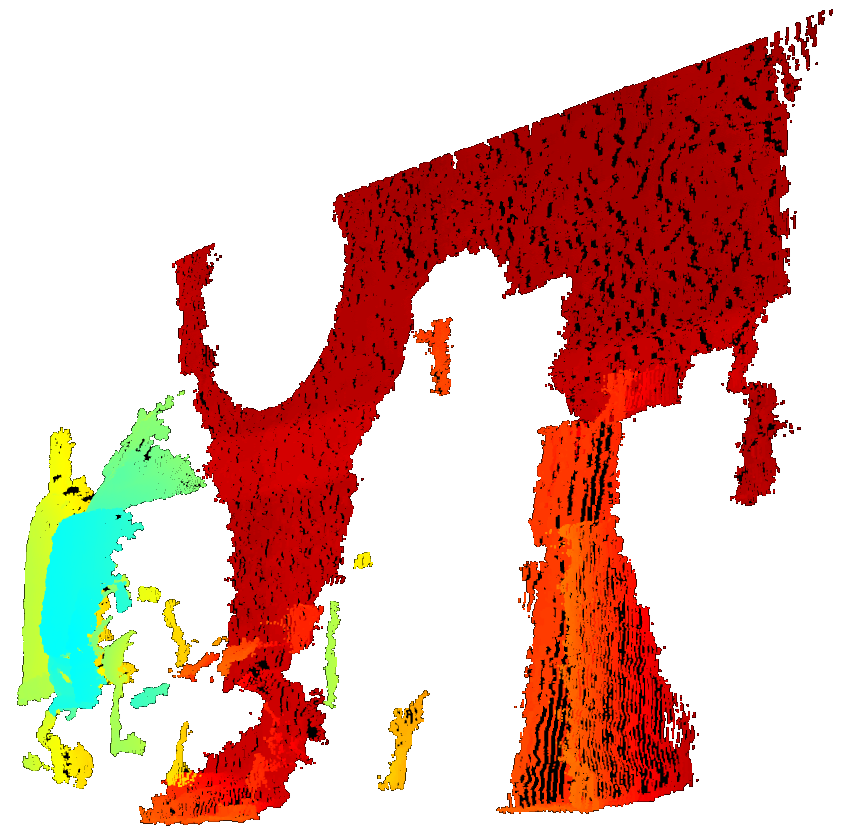
\includegraphics[width=1.0\linewidth]{figures/background_3dpc_example.png}
                    
                    \captionsetup{singlelinecheck=false, justification=raggedright}
                    \caption{Example of a \gls{3DPC} acquired on a Microsoft Kinect camera.}
                    \label{fig:external_devices_3dpc_example}
                \end{figure}
                
                There are numerous external device methods used to track the patient and acquire a \gls{SS}.  Four example devices are:
                
                \begin{itemize}
                    \item Firstly, the oldest method of \gls{SS} tracking presented here is the use of a spirometer. A spirometer is a device with a tube which is inserted into the mouth of the patient through which they breath. The spirometer measures the volume of air and the velocity with which the patient inhales or exhales~\boxcite{Guivarch2004SynchronizationPlethysmography}. Some disadvantages of this method include; %that it is difficult to temporally synchronise the acquisition of the \gls{PET} data with the data from the spirometer. Additionally,
                    because spirometers are not designed for highly accurate measurement, over time, they are susceptible to value drift where the mean position of the respiratory cycle is not consistent between cycles~\boxcite{Hoisak2004}.
                    
                    \item Secondly, a method borrowed from radiotherapy for \gls{SS} tracking is through the use of the Varian \gls{RPM}. The \gls{RPM} was designed to be used in radiotherapy to turn on and off the beam of a linear accelerator. This would work by using the infrared camera of the \gls{RPM} to track a reflective marker placed on the stomach or chest of the patient, tracking the displacement of the chest wall over time. This can be seen in~\Fref{fig:external_devices_rpm}. The Anzai AZ-733V system attempts to acquire the displacement of the abdomen, similarly to the \gls{RPM}, but uses a pressure belt wrapped around the patient. In radiotherapy, as the patient moves the target of the linear accelerator also moves so the beam is only turned on when the target is within a set range. In \gls{PET} the \gls{RPM} has been modified to output a clock tick to the computer acquiring the \gls{PET} data, this computer will %then synchronise with the \gls{RPM} clock and 
                    record timing information into the \gls{PET} data in order to align the \gls{RPM} \gls{SS} post acquisition. This method has the advantage over the spirometer in that it is significantly less susceptible to drift. However, the use of the \gls{RPM} increases scan time and as such receives push back from radiographers.
                    
                    \item Thirdly, optical or laser based cameras, such as the Microsoft Kinect, can be used to determine a segmentation of the patient or (using the \gls{TOF} of lasers to determine depth) a \gls{3DPC} of the patient, at each time point. An example of a \gls{3DPC} acquired on a Microsoft Kinect camera can be seen in~\Fref{fig:external_devices_3dpc_example}. A \gls{3DPC} is a collection of coordinates measured as points on the surface of the object being scanned at some displacement. A \gls{SS} can be acquired by finding the difference in these segmentations or \glss{3DPC} over time~\boxcite{Miranda2017MarkerlessAnimals}. Advantages of this solution include; it doesn't make use of a reflective marker placed on the patient, like the \gls{RPM}, and as such shouldn't increase scan time. Additionally, an optical or laser based camera can track motion over a larger \gls{FOV} than the \gls{RPM}, for instance, an optical or laser based camera could conceivably simultaneously track both respiratory and head motion, producing directly a \gls{DVF} or separate \glss{SS}. A disadvantage is that it is much more difficult to spatially and temporally align the acquisition of both a \gls{PET} scanner and a stand alone optical or laser based camera~\boxcite{Noonan2012AccurateKinect}~\boxcite{Noonan2015RepurposingPET}~\boxcite{Whitehead2018MotionPET/CT}.
                    
                    \item Finally, on \gls{MR} scanners, there is the \gls{MR} navigator. During an \gls{MR} protocol there are times when the \gls{MR}, if told to do so, can measure specific small areas of the patient's anatomy. An \gls{MR} navigator can be used to measure a pencil shaped \gls{1D} area, for instance, the position of the diaphragm or the chest wall of the patient~\boxcite{Taylor1997MRAngiography}. An advantage of this is that multiple navigators can be placed to track more than one \gls{SS}. This works by looking for edges along the \gls{1D} pencil and assuming that the edge reflects the current position of the diaphragm or chest wall. An advantage of this is that it does not require any other additional equipment other than the \gls{MR} scanner and does not significantly affect scan time. A disadvantage is that it requires a \gls{MR} scanner which is not available during \gls{PET}/\gls{CT}.
                \end{itemize}
                
            \subsubsection{Data Driven} \label{sec:data_driven}
                \begin{figure}
                    \centering
                        
                    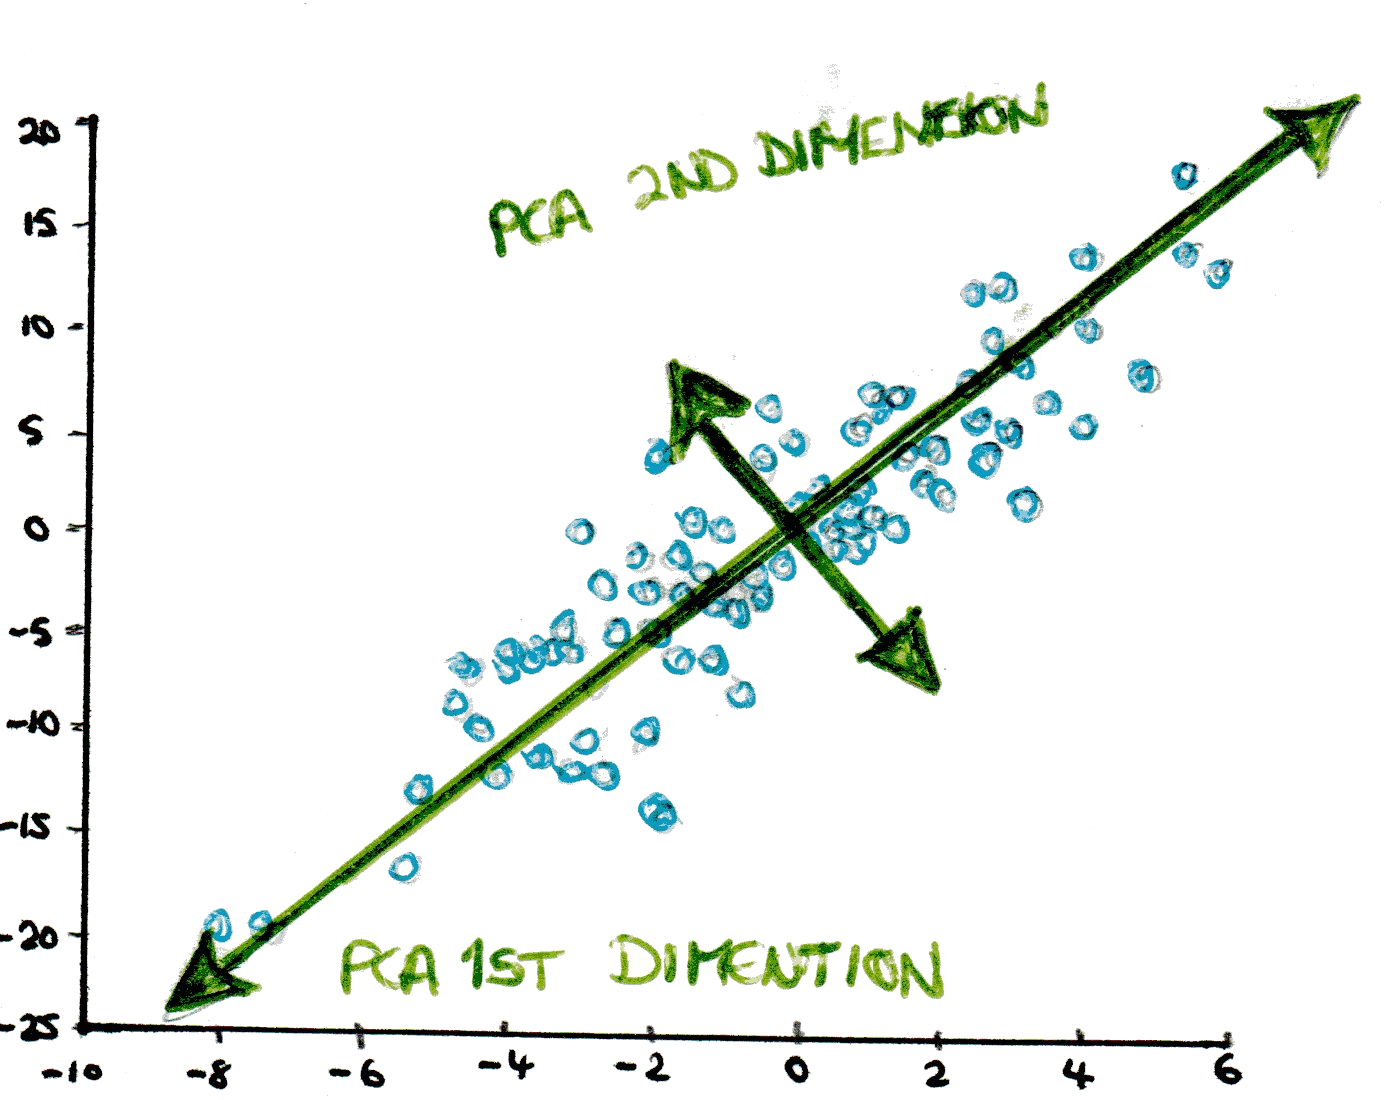
\includegraphics[width=1.0\linewidth]{figures/background_pca.png}
                        
                    \captionsetup{singlelinecheck=false, justification=raggedright}
                    \caption{Graphical representation of \gls{PCA} applied to \gls{2D} data. In the centre the \gls{2D} data points on which \gls{PCA} has been applied can be seen. From bottom left to top right the first eigenvector can be seen with most variance, from top left to bottom right the second eigenvector can be seen with less variance.} \label{fig:data_driven_pca}
                \end{figure}
                
                \begin{figure}
                    \centering
                        
                    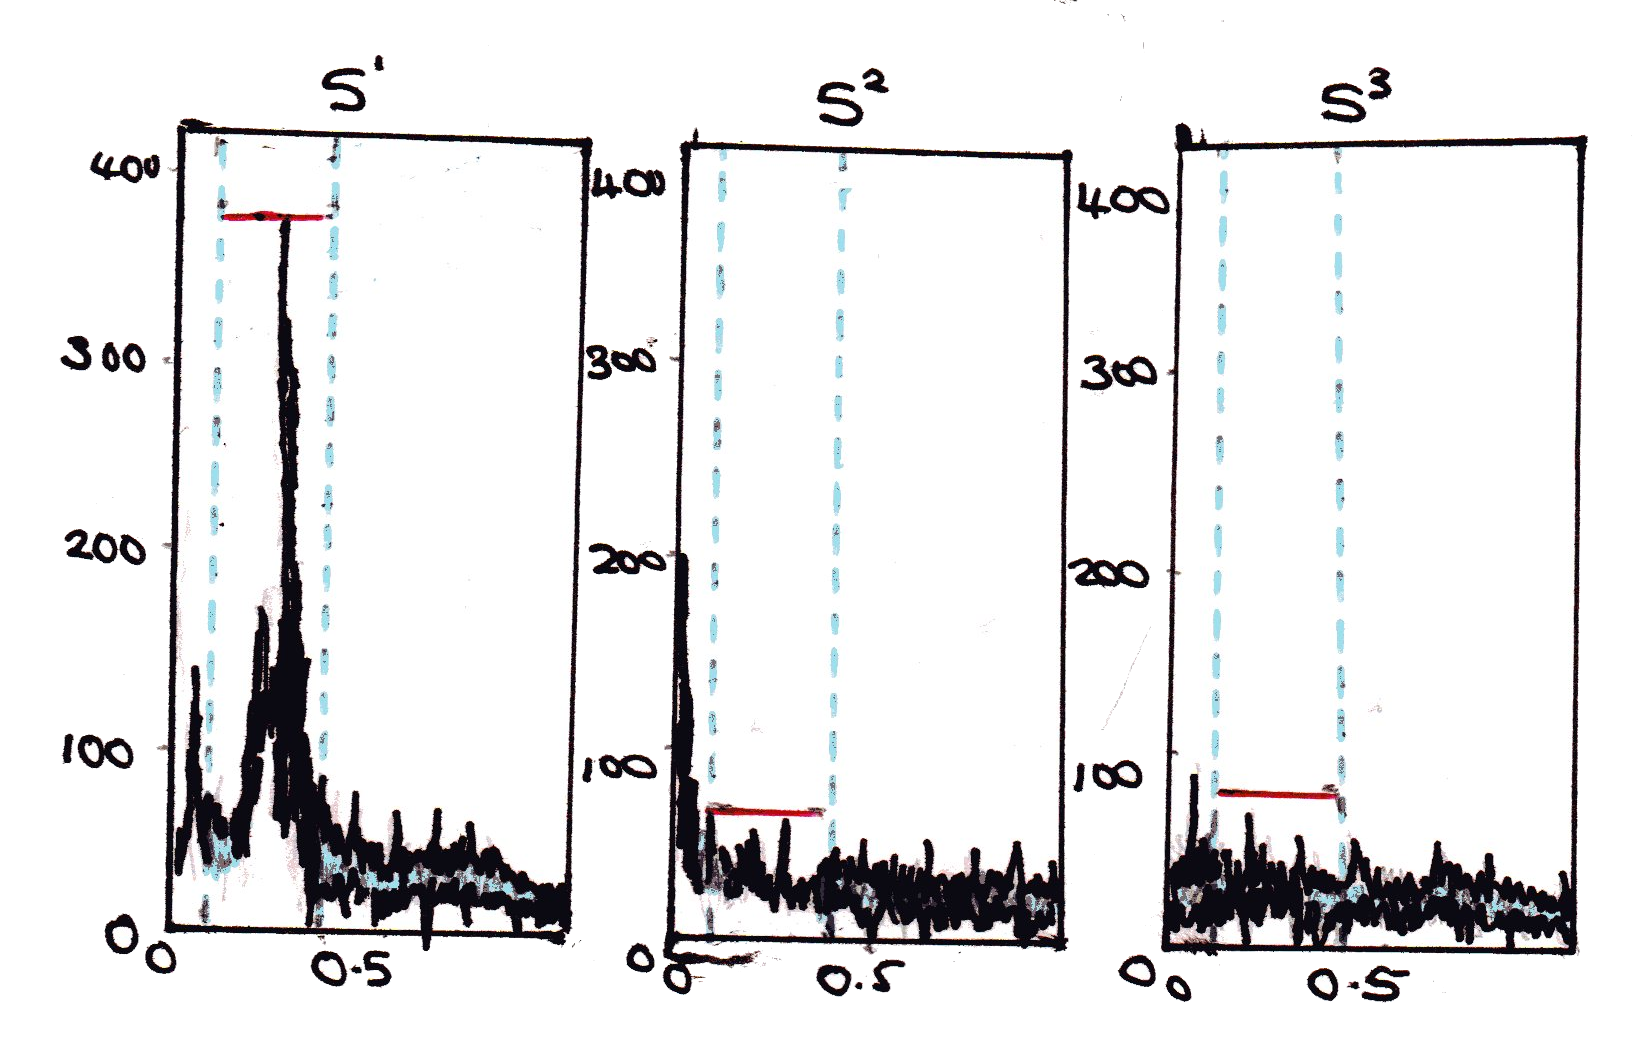
\includegraphics[width=1.0\linewidth]{figures/background_pca_window.png}
                        
                    \captionsetup{singlelinecheck=false, justification=raggedright}
                    \caption{Graphical representation of the frequency spectrum for three \gls{PC}. On the right a frequency spectrum of one \gls{PC} with a frequency window between \SI{0.1}{\hertz} and \SI{0.4}{\hertz} and a low value peak in this window can be seen. In the centre another example of what can be seen on the left can be seen. On the left another frequency spectrum with a frequency window can be seen, however, here the peak in the frequency window is significantly higher than in the other two examples.} \label{fig:data_driven_pca_window}
                \end{figure}
                
                There are numerous \gls{DD} methods used to extract a \gls{SS} directly from \gls{PET} data. Some methods require that the \gls{PET} data be reconstructed first and then markers, possibly inserted into the patient, are tracked over time. Methods requiring reconstruction are mostly inferior to methods which work on \gls{PET} acquisition data. This is because requiring that reconstruction be performed takes significant time and the \gls{SS}, itself, is usually required for most \gls{MC} methods so the initial reconstructions will be poor. Here, of the methods using \gls{PET} acquisition data, only \gls{PCA} will be discussed as it has been proven that most static \gls{DD} \gls{SS} extraction methods perform similarly~\boxcite{2013ComparisonData}. Additionally, \gls{PCA} is the method of choice on \gls{GE} scanners.
                
                \gls{PCA} is a dimensionality reduction technique, closely related to \gls{SVD}, which attempts to find a transformation that maps the data to a lower dimensional space where the underlying structure of the data can be better determined~\boxcite{Pearson1901LIII.Space}. \gls{PCA} produces, for the data, a series of eigenvectors and weights where the eigenvectors are the orthogonal vectors of descending variance through the data (usually normalised) and the weights are the magnitude of these eigenvectors apparent in the data, this can be seen in~\Fref{fig:data_driven_pca}. Thus the first eigenvector from \gls{PCA} will represent the vector of greatest variance through the data, in thoracic \gls{PET} this will usually be caused by the \gls{RM} of the patient, but is not always.
                
                When applied specifically to \gls{PET} acquisition data (following~\boxcite{Thielemans2011}) \gls{PCA} is often used on either sinograms or unlisted listmode data, the resultant sinograms are usually spatially downsampled. This is for a number of reasons including; the noise present in the full data would obscure the motion. Additionally, the large size of the \gls{PET} sinograms provides issues when it comes to storing the number needed in memory and the computational expense necessary to apply \gls{PCA}, generally all of the data, which the method will be applied to, must be in memory simultaneously. Furthermore, the non-downsampled sinograms contain more than enough information than is required for \gls{PCA} to be able to extract the relevant variation, thus if all the data was used then time would be wasted processing this data. Generally additional filtering (or smoothing) can be applied and in most cases will, in fact, improve results (see~\Fref{sec:pca_data_driven_surrogate_signal_extraction_methods_for_dynamic_pet_methods}). Usually when used to extract respiratory variation the sampling rate of the \gls{PET} sinograms is chosen as \SI{0.5}{\second} so as to attempt to mitigate cardiac motion by averaging most of it in each frame while still allowing for \gls{RM} between frames~\boxcite{Bertolli2018Data-DrivenTomography}.
                
                The \gls{PC} which contains the variation present in the data caused by \gls{RM} must be identified. One method to do this is as follows; first, the frequency spectrum of the weight of each \gls{PC} is required, this shows at what frequency variation occurs along the weight of each \gls{PC}. Then a frequency window is determined, this is usually between \SI{0.1}{\hertz} and \SI{0.4}{\hertz} so as to coincide with the approximate frequency of respiration. The max value or peak in the frequency spectrum is then found for each \gls{PC} in this window. The \gls{PC} which has the largest peak in the window is determined as being the one best representing variance caused by \gls{RM}, this can be seen in~\Fref{fig:data_driven_pca_window}~\boxcite{Thielemans2011}.
                
                Evaluations have been performed on static PET data \gls{18F-FDG} to compare the results of the \gls{DD-PCA} to both \gls{RPM} and \gls{MR} navigator based \glss{SS}. When compared to both external methods \gls{DD-PCA} was shown to be relatively robust, specifically showing a correlation of $0.89$ over nine patients when compared to the \gls{MR} navigator based \glss{SS}~\boxcite{2013ComparisonData}~\boxcite{Manber2015PracticalPET/MR.}.
                
                An advantage of the \gls{PCA} based \gls{SS} extraction method over external device based \gls{SS} tracking is that the \gls{PCA} method allows for \gls{SS} extraction at any point during the scan, once \gls{PET} acquisition data has been acquired of the thorax, even post scan. \gls{DD-PCA} can be applied automatically without the intervention of a clinician, nor radiographer, thus not affecting acquisition time or inserting additional steps into clinical practise. \gls{DD-PCA} is also usually more comfortable for the patient as it does not involve any effort from them, in either being strapped into or otherwise having to interact with a device. This is all the while, as discussed above, providing accurate results when compared to the external devices. Additionally, \gls{DD-PCA} does not require any other modality, like \gls{MR} navigators, and as such is universally appropriate wherever \gls{PET} acquisition data is available. However, it should be noted that the \gls{SS} acquired will vary depending on the modality it is applied to, for instance, if \gls{DD-PCA} were applied to \gls{CT} data rather than \gls{PET} then the values would not be comparable.
                
                An additional issue with \gls{DD-PCA}, when applied to dynamic \gls{PET}, is that it is sensitive to dynamic tracer kinetics from dynamic \gls{PET} scans, as discussed in~\Fref{sec:static_and_dynamic_acquisition}. This means that while tracer kinetics are apparent in the data they will cause significantly more variation than \gls{RM} would do and thus mask the respiratory \gls{SS} derived via \gls{DD-PCA}. It is also not the case that the whole of the respiratory variation would be displaced to another \gls{PC}, generally its variation is mixed with the variation cause by the tracer kinetics and obscured. This will be investigated further in~\Fref{sec:data_driven_surrogate_signal_extraction_results}
        
        \subsection{Applying Image Registration} \label{sec:applying_image_registration}
            \begin{figure}
                \centering
                        
                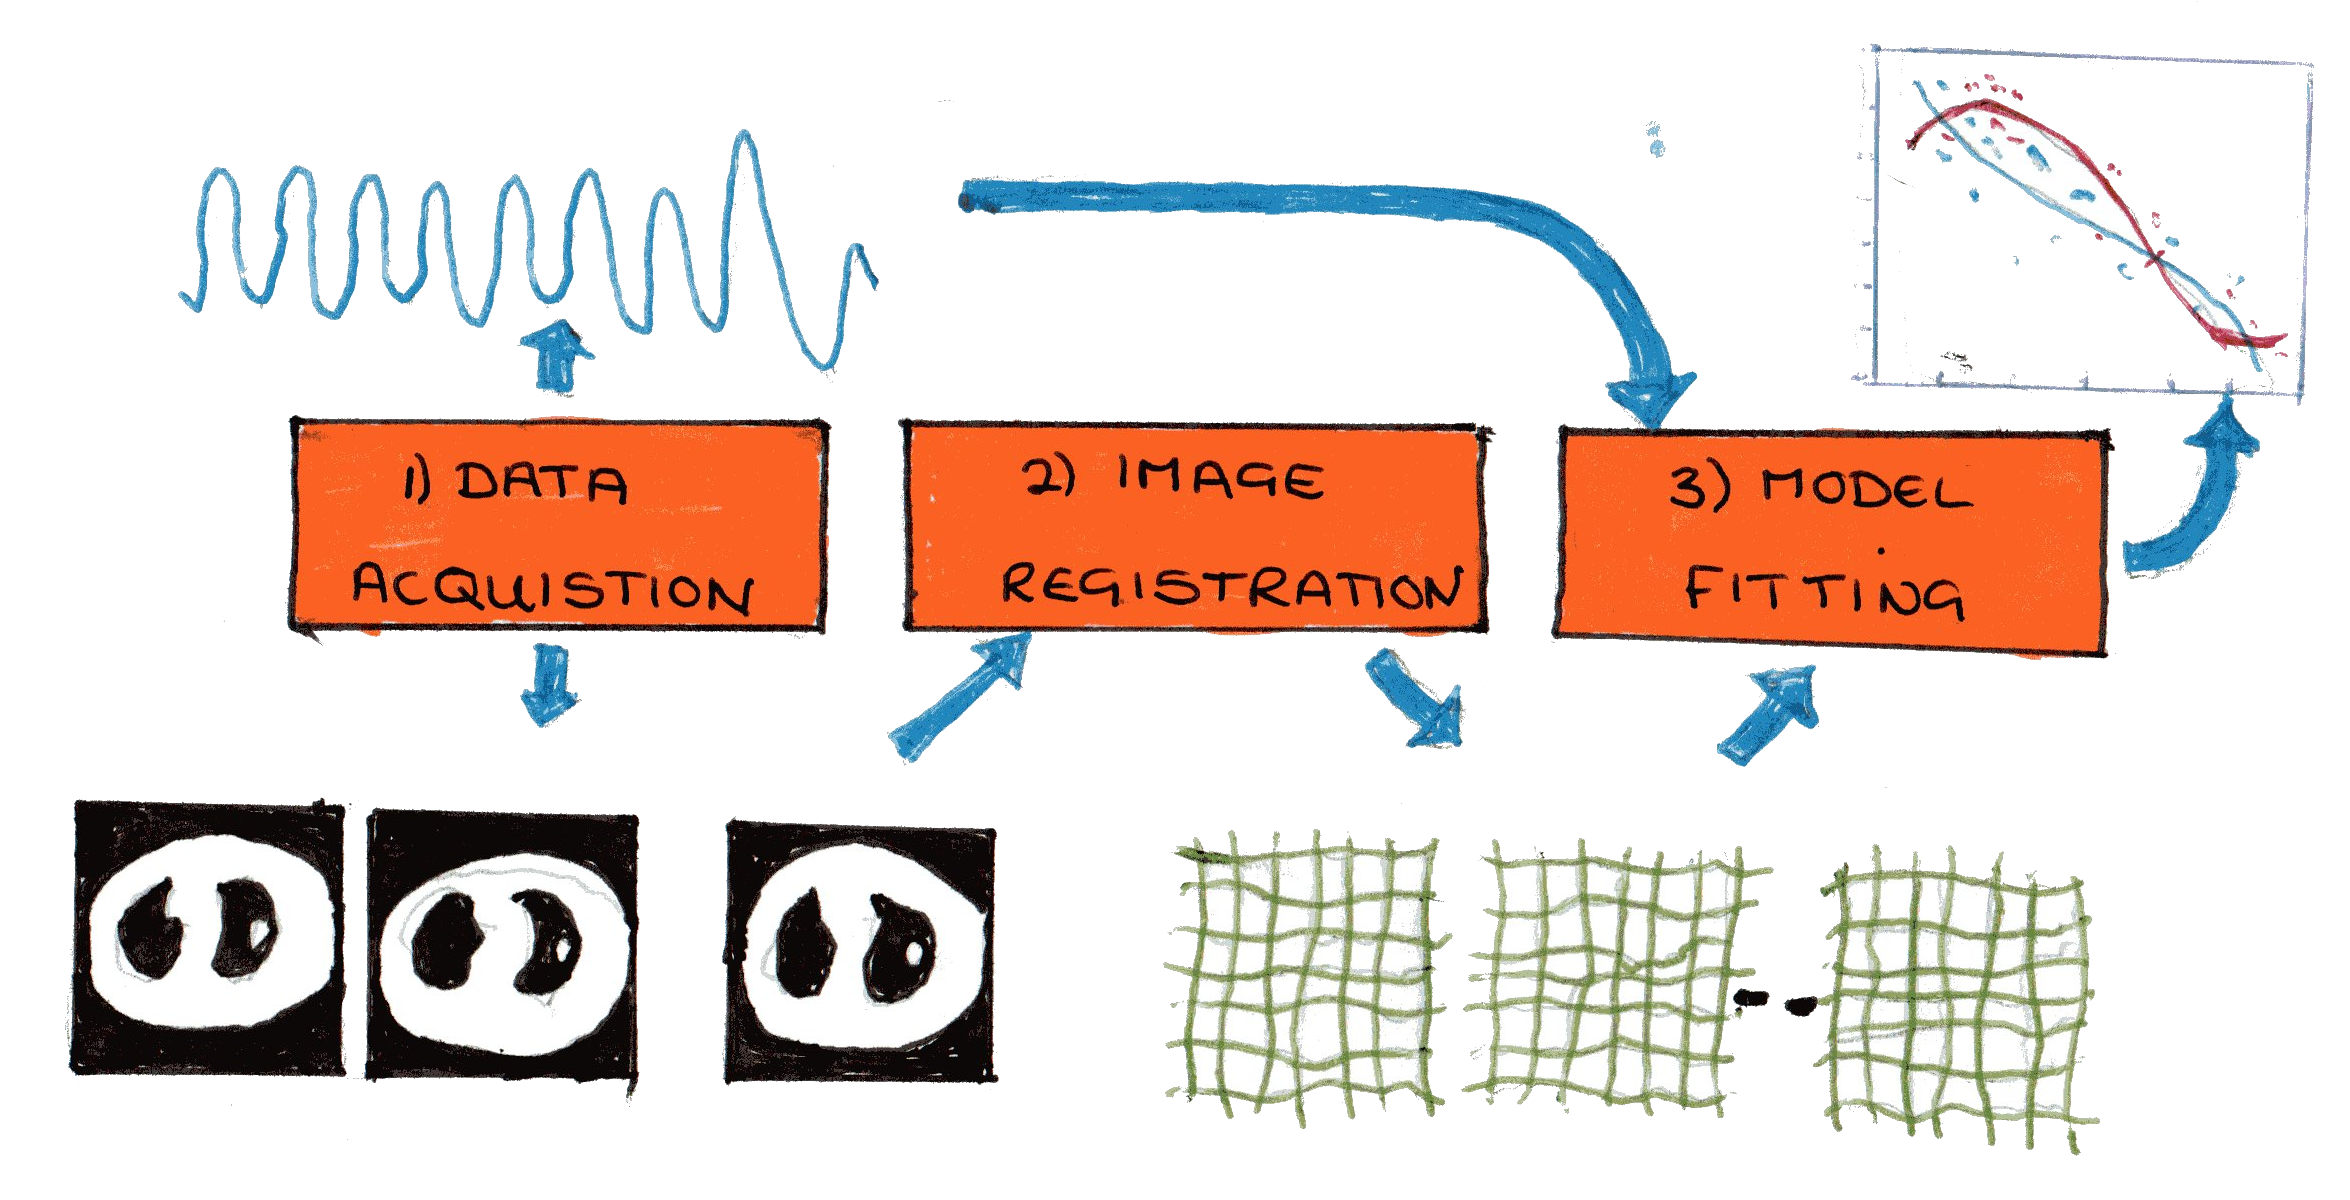
\includegraphics[width=1.0\linewidth]{figures/background_motion_model.png}
                        
                \captionsetup{singlelinecheck=false, justification=raggedright}
                \caption{Graphical representation of . On the left .} \label{fig:applying_image_registration_pairwise_groupwise_comparison}
            \end{figure}
            
            \begin{figure}
                \centering
                        
                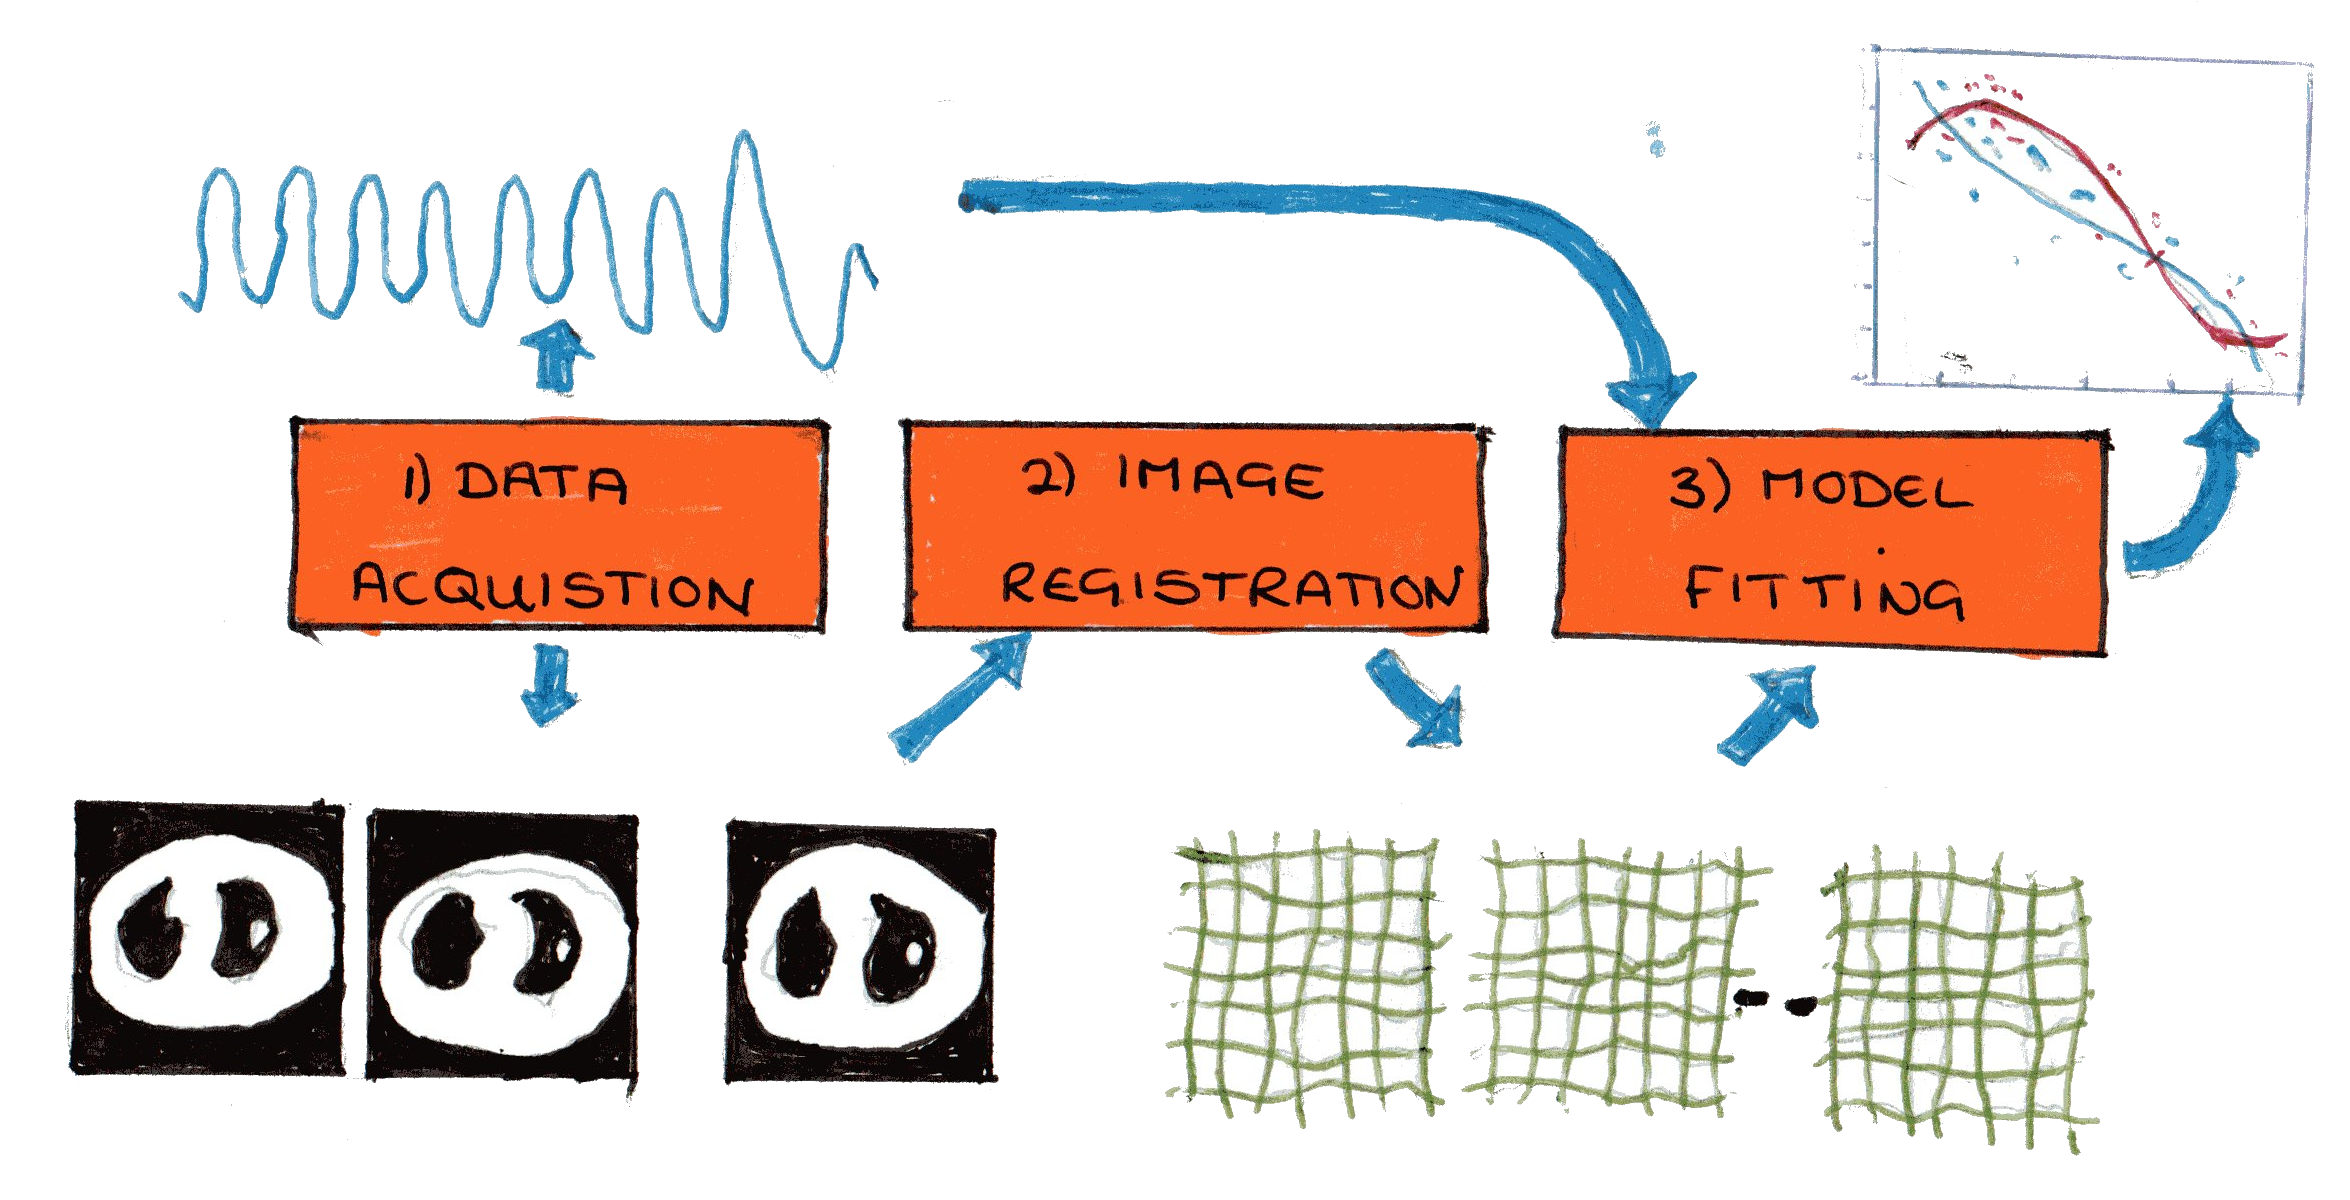
\includegraphics[width=1.0\linewidth]{figures/background_motion_model.png}
                        
                \captionsetup{singlelinecheck=false, justification=raggedright}
                \caption{Graphical representation of . On the left .} \label{fig:applying_image_registration_groupwise_breakdown}
            \end{figure}
            
            There are multiple ways to write an algorithm to \gls{MC} a series of respiratory gated \gls{PET} volumes incorporating \gls{IR}. Two of the most common are as follows:
            
            \begin{itemize}
                \item Firstly, pairwise registration, here one of the gates is selected and all other gates are registered to it. Usually the gate with the highest number of counts is selected due to it having the highest \gls{SNR}. Once \gls{IR} is complete each gate is resampled using the corresponding \gls{DVF} and summed to form the final \gls{MCI}. An advantage of this algorithm is that it is relatively simple, usually only one pass of \gls{IR} is required and thus it could be considered relatively quick. However, the accuracy of the \gls{MC} entirely hinges on the quality of the volume selected as the reference, if it is low quality then it would be difficult to accurately register the gates. Additionally, the reference gate may be far from a number of the other gates if the reference is close to max inhalation or exhalation (compounded with a large amount of the anatomy possibly being outside the \gls{FOV} if the reference is close to max inhalation) again hindering the ease of registration.
                
                \item Secondly, groupwise registration, Here all gates are summed to form a reference volume. Gates are registered to the reference, resampled and summed once more to form a new reference volume, this process is performed a set number of times, with the quality of the reference, ideally, increasing each time. As an additional step the inverse mean of all \glss{DVF} can be composed with each \gls{DVF} before resampling the gates to ensure that the reference gate is at the mean respiratory position. A graphical representation of groupwise registration can be seen in~\Fref{fig:applying_image_registration_groupwise_breakdown}. An advantage of this algorithm is that it has the capacity to provide better registration results due to the higher \gls{SNR} of the reference volume. However, it can also take longer to perform due to the multiple full iterations of \gls{IR}
            \end{itemize}
            
            A graphical comparison of pairwise and groupwise registration can be seen in~\Fref{fig:applying_image_registration_pairwise_groupwise_comparison}.
            
        \subsection{Motion Modelling} \label{sec:motion_modelling}
            \begin{figure}
                \centering
                        
                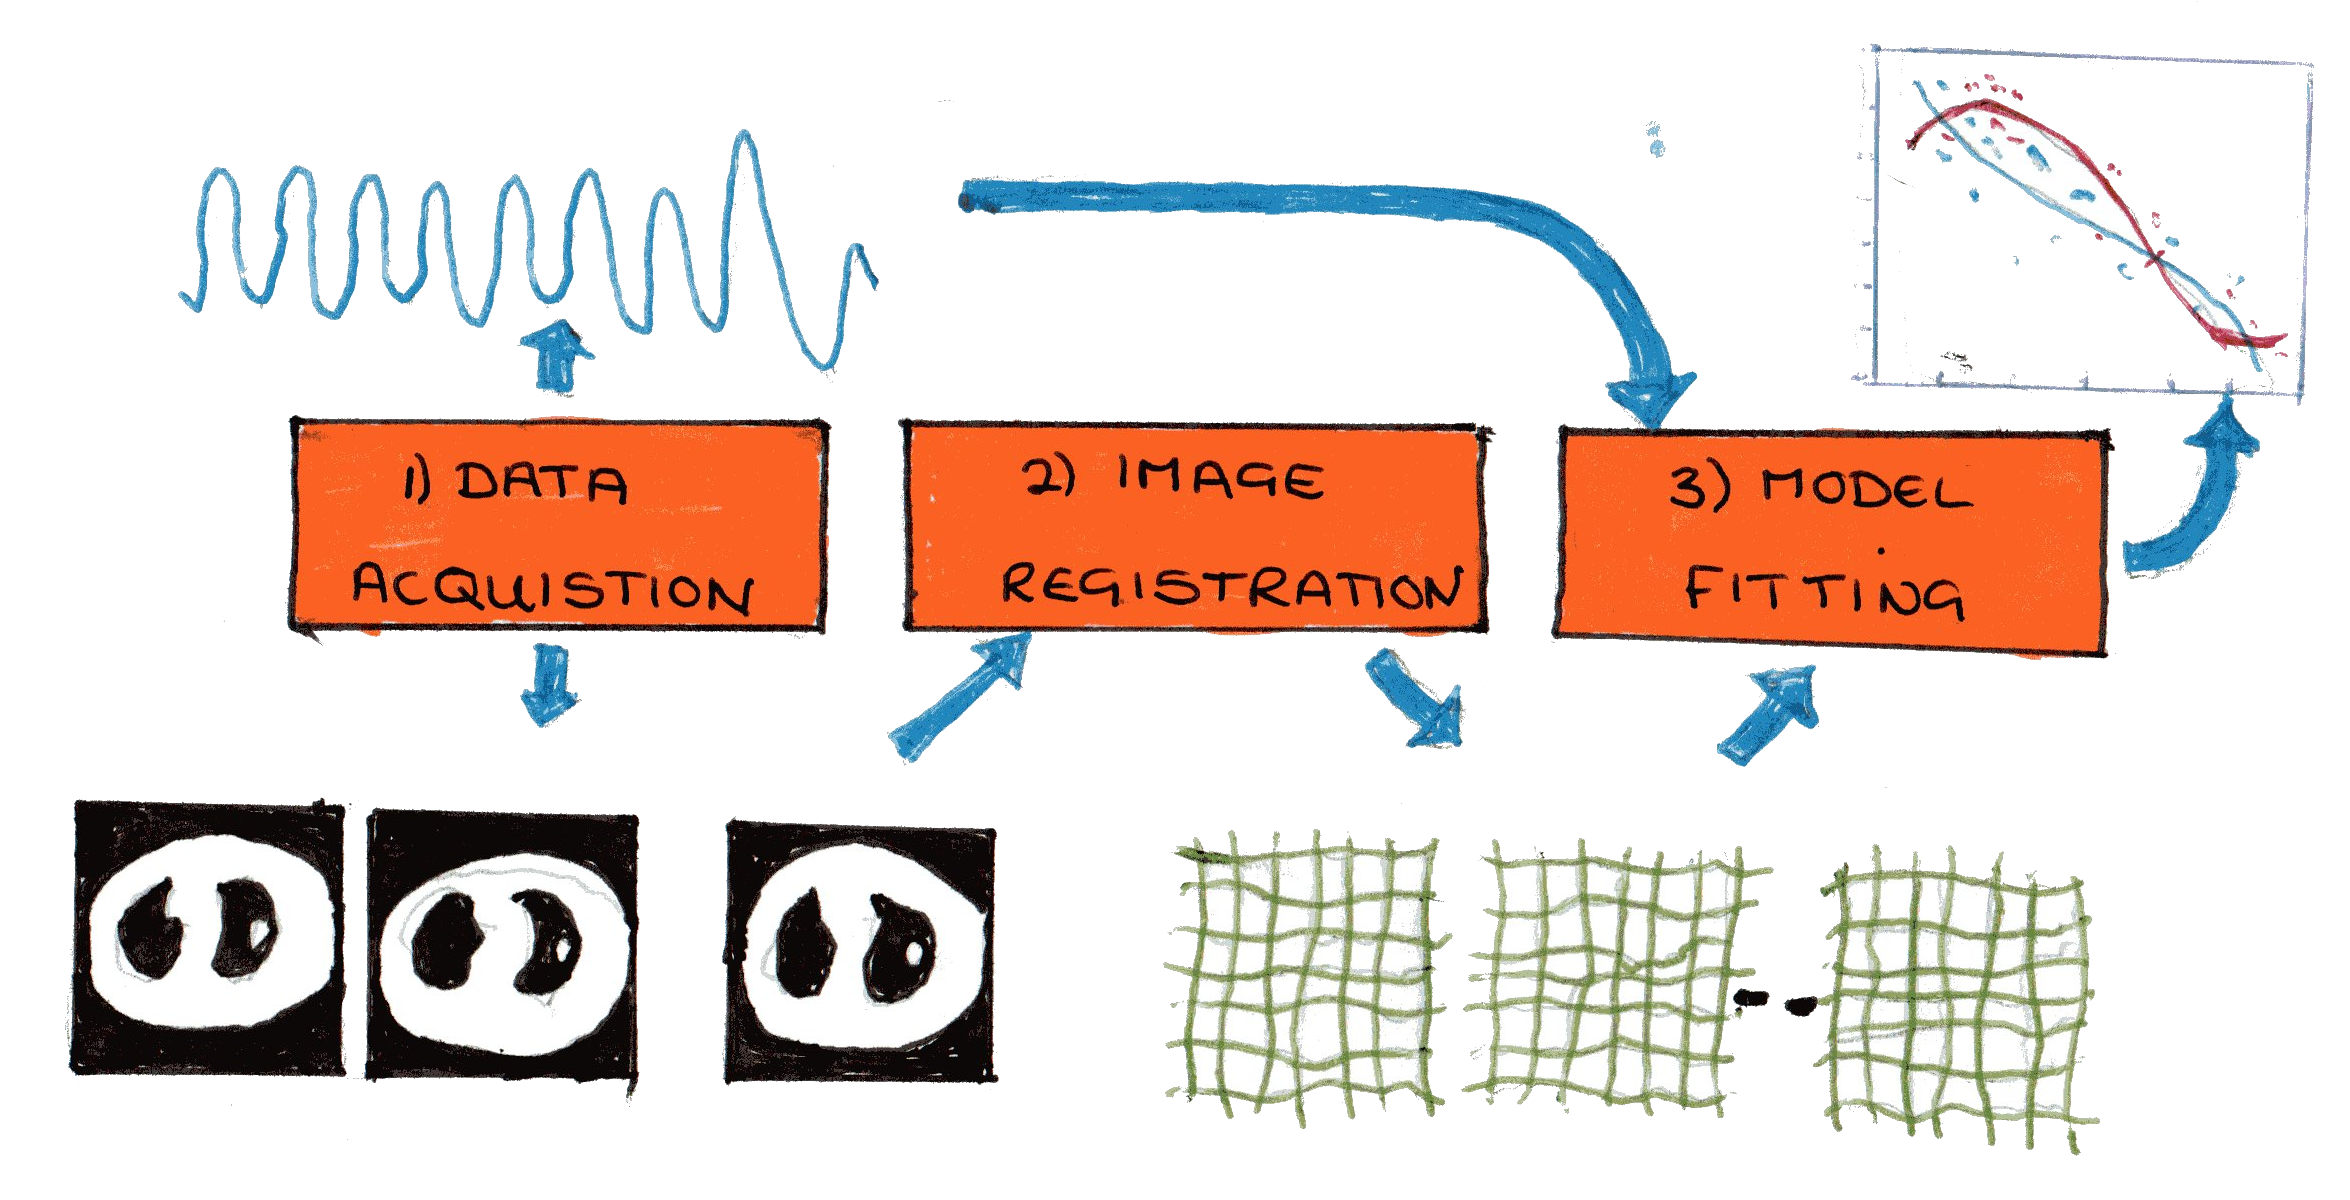
\includegraphics[width=1.0\linewidth]{figures/background_motion_model.png}
                        
                \captionsetup{singlelinecheck=false, justification=raggedright}
                \caption{Graphical representation of the process of \gls{MM}. On the left the initial data acquisition of both the data and the \gls{SS} can be seen. Then in the centre the data is taken and an \gls{IR} is applied to it. Then on the right it can be seen that the \gls{SS} is taken again and a \gls{RCM} is fit on it and the \gls{DVF} from \gls{IR}. In the top right a naive example of the \gls{2D} regression fit can be seen.} \label{fig:motion_modelling_motion_model}
            \end{figure}
            
            \glss{MM} offer an alternative solution to \gls{MC} when compared to vanilla co-registration of respiratory gated \gls{PET}. \glss{MM}, similarly to the \gls{RPM} discussed in \Fref{sec:external_devices}, is a technique borrowed from radiotherapy. \glss{MM} themselves attempt to relate the \glss{DVF} or \gls{BS} \gls{CPG} from, for instance, \gls{IR} to the \gls{SS} acquired for the data used to generate the \glss{DVF}. In this case a \gls{RCM} would be generated which is fit on the \glss{DVF} and \gls{SS}, this can be seen in~\Fref{fig:motion_modelling_motion_model}. In its simplest form a post \gls{IR} \gls{MM} could be a linear regression of both the \glss{DVF} and the \gls{SS}. In the case described previously the \glss{DVF} are found first before fitting the \gls{RCM}, however, in more resent research a method to simultaneously fit both the \gls{BS} \gls{CPG} and the \gls{RCM} has been presented~\boxcite{McClelland2013}~\boxcite{McClelland2006}~\boxcite{McClelland2014}~\boxcite{McClelland2017}.
            
            There are four components required to perform \gls{MM}, these are; the data itself which is to be \gls{MC}, a \gls{SS} with an value representing the respiratory position at each data point (the \gls{SS} can be \gls{ND}), the \glss{DVF} for each piece of data (or \gls{BS} \glss{CPG}) and the \gls{RCM} linking the \glss{DVF} and \gls{SS}.
            
            An advantage of \gls{MM} over vanilla co-registration is that it allows for prediction of data not used to fit the \gls{RCM}, this advantage is particularly useful for radiotherapy. Here, some data is acquired on the machine used to perform radiotherapy (usually on the patient on the day of therapy). This allows for a \gls{RCM} to be fit (pre-therapy) on the data acquired with a \gls{SS} from, for instance, the \gls{RPM}. Then, as a dose is administered to the patient, from a linear accelerator, \glss{SS} values can continue to be acquired and \glss{DVF} calculated using the \gls{RCM} fit previously in order to, in real time, change the trajectory of the linear accelerator to apply a dose only in the \gls{ROI}. The new \gls{SS} values need not match any of the \gls{SS} values used to generate the \gls{RCM} as the \gls{RCM} is a continuous model. This advantage could provide the ability in \gls{PET} to calculate a \gls{RCM} while acquisition is still ongoing to be used for \gls{MC} during reconstruction (or indeed for a \gls{RCM} to be fit on a subset of the data to improve \gls{MC} speed).
            
            An additional advantage of \gls{MM} is that compared to vanilla co-registration it is more robust to noise. This is because vanilla co-registration will register each individual volume together (regardless of how well that registration fits the underlying motion of the patient) whereas \gls{MM} will then either be fit on top of (or be applied simultaneously with) registration using the \gls{SS} regularising the effect of outlying data points and noise in general.
            
            \subsubsection{Respiratory Correspondence Model} \label{sec:respiratory_correspondence_model}
                \begin{figure}
                    \centering
                            
                    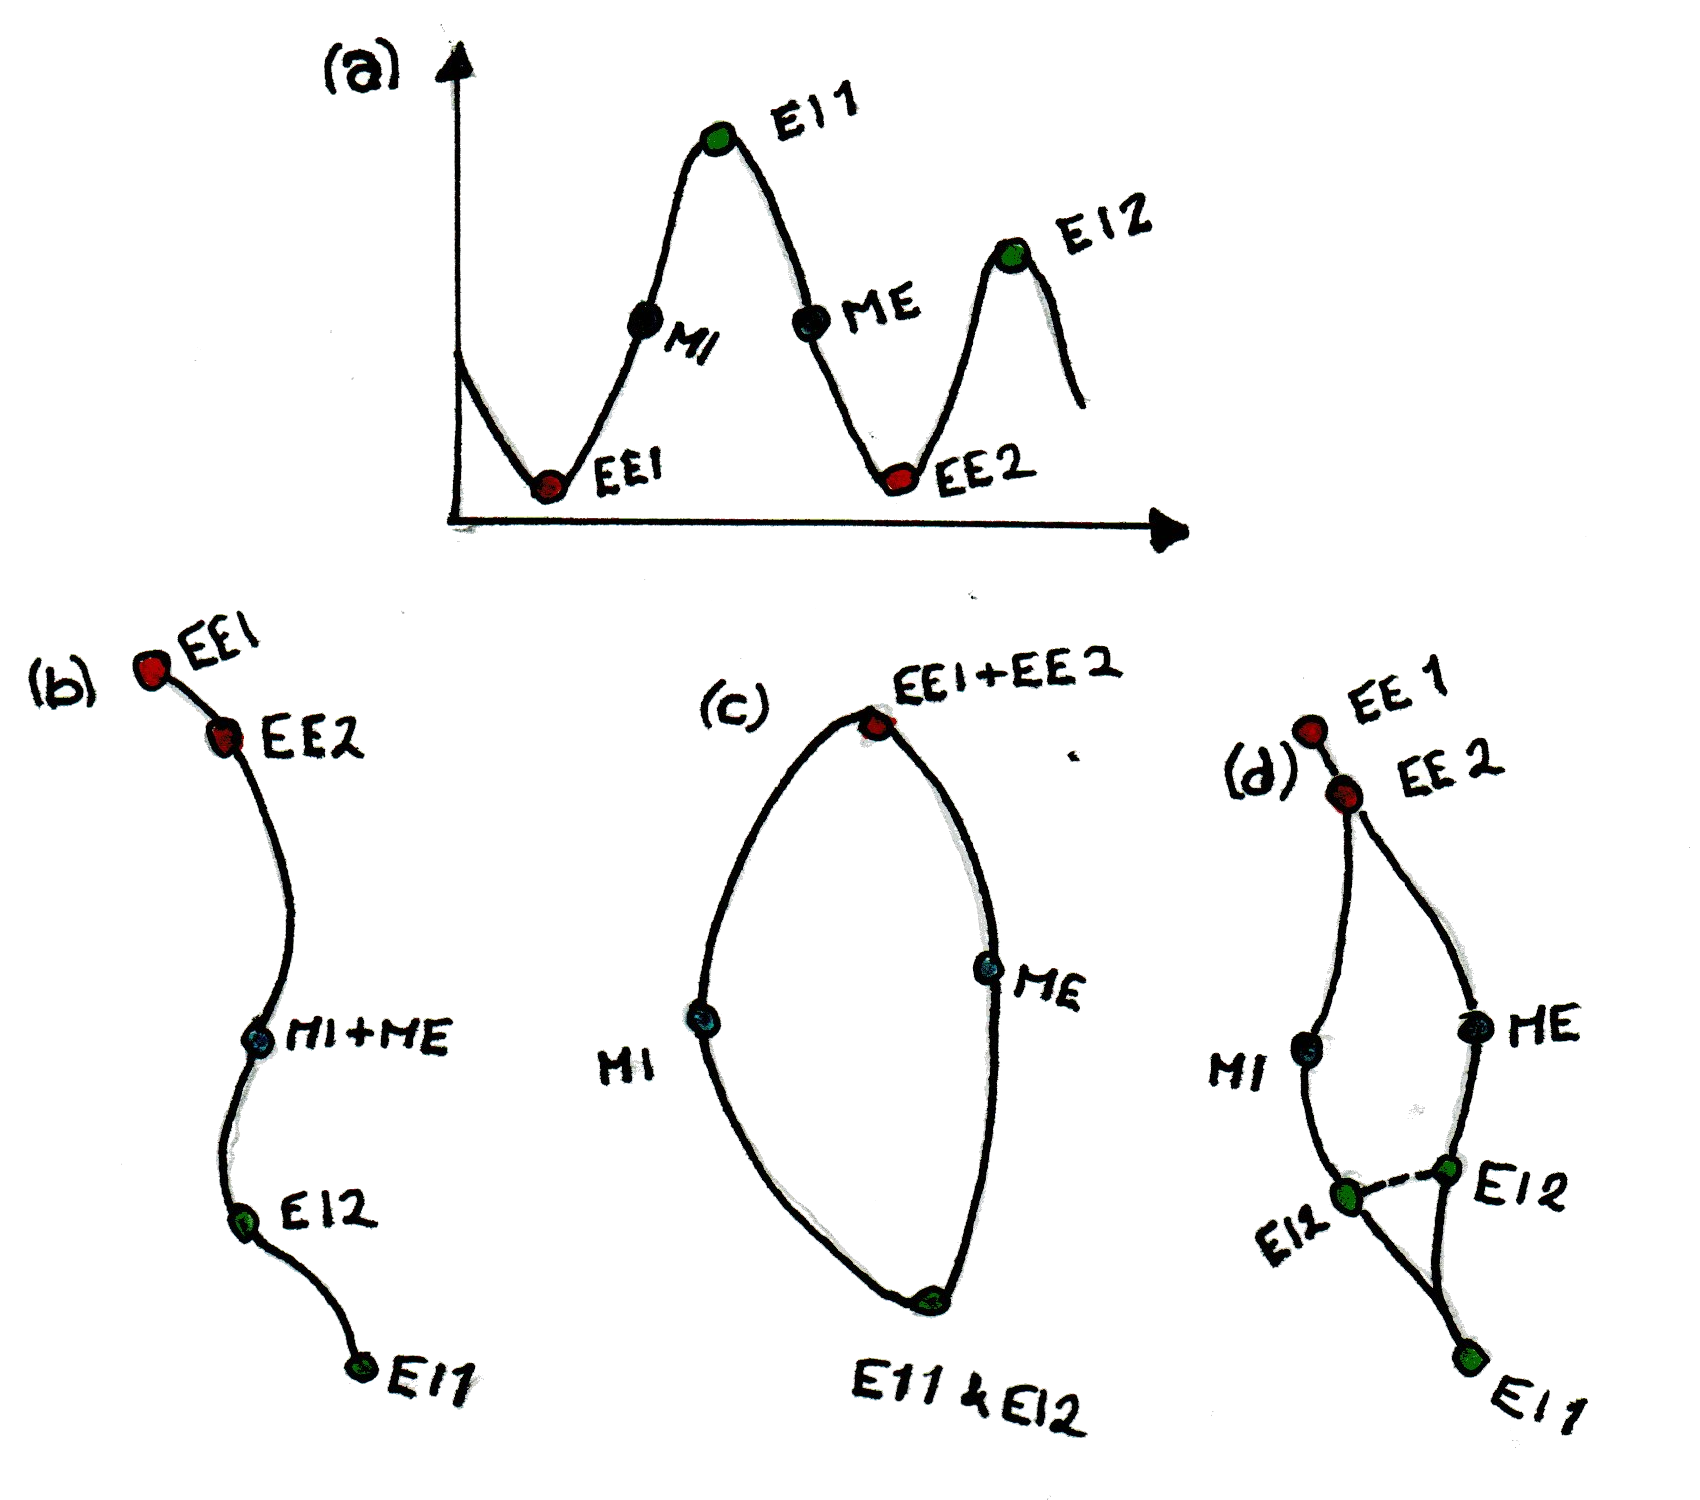
\includegraphics[width=1.0\linewidth]{figures/background_rcm.png}
                            
                    \captionsetup{singlelinecheck=false, justification=raggedright}
                    \caption{Graphical representation of the types of \gls{RCM}. At the top of the figure is a \gls{SS} which has been discretised into specific values. On the bottom left is a linear \gls{RCM} showing how the points from the discretised \gls{SS} would be mapped to itself. On the bottom middle is a cyclical \gls{RCM} and on the bottom right is an \gls{RCM} where inhalation and exhalation are modelled separately from one another.} \label{fig:motion_modelling_rcm}
                \end{figure}
                
                The type of \gls{RCM} fit depends mostly upon the \gls{SS} given to the \gls{MM} algorithm, some of the different types of \gls{RCM} can be seen in~\Fref{fig:motion_modelling_rcm}. The most simple forms of \gls{RCM} would be both the linear and cyclical \gls{RCM}. To fit a linear \gls{RCM} a \gls{SS} representing the amplitude of respiration should be given. A disadvantage of a linear \gls{RCM} is that inhalation and exhalation are treated alike when in reality they differ. A cyclical \gls{RCM} is often fit using the phase of respiration as the \gls{SS}. A disadvantage of this type of \gls{RCM} is that it treats every breath as if it is exactly the same regardless of the max displacement of the breath. A final, more complex, \gls{RCM} is one where it is fit not only on the amplitude of respiration but also the gradient of the \gls{SS}, this would mean that the \gls{RCM} can model both inhalation and exhalation separately. However, moving from inhalation to exhalation may incur a 'jump' in the output from the \gls{RCM}~\boxcite{McClelland2013}.
                
                The reference position of the \gls{SS} with regards to the \gls{RCM} can be defined in two ways:
            
                \begin{itemize}
                    \item One, the reference position is defined as the mean respiratory position. This is similar to how the reference position is defined for groupwise registration, as discussed in~\Fref{sec:applying_image_registration}. A value of zero for the surrogate signal would correspond to the respiratory position which is in the 'centre' of all the input data.
                    
                    \item Two, if an additional dimension is added to the \gls{SS}, which does not vary, it allows the intercept of the \gls{RCM} to be fit. Thus the reference position does not need to sit at the mean respiratory position, which may in some applications be useful, for instance, if the reference position was set as the position of the \gls{Mu-Map}.
                \end{itemize}
                
        
        \subsection{Applying Motion Correction} \label{sec:applying_motion_correction}
            As discussed throughout this chapter, in~\Fref{sec:respiratory_motion_challenges_in_combined_pet_ct_imaging} and~\Fref{sec:respiratory_gating}, there are a number of methods through which the \glss{DVF}, found from vanilla \gls{IR} or \glss{MM}, can be applied to the task of \gls{MC}. These methods mostly fit into two different classes, these are:
            
            \begin{itemize}
                \item Firstly, post reconstruction \gls{MC}. Here the \glss{DVF} are acquired and used to warp the results of \gls{PET} reconstruction once after all iterations of the reconstruction algorithm have finished. Usually \gls{IR} is performed in image space using an objective function such as \gls{MI} of \gls{MSE}, discussed in~\Fref{sec:image_registration}. An example of a post \gls{IR} \gls{MC} technique would be performing respiratory gating, reconstructing the gated volumes and then registering and summing all gates together, this was discussed briefly in~\Fref{sec:respiratory_motion_challenges_in_combined_pet_ct_imaging}. This method has the advantage that it is relatively simple to implement, each section of reconstruction and \gls{MC} is separate and sequential. Because of this the algorithm is more stable and few iterations of \gls{MC} are preformed.
                
                \item Secondly, iterative reconstruction and \gls{MC}. This class of \gls{MC} techniques take the optimisation for reconstruction and \gls{MC} and iterates between them. An example of an iterative reconstruction and \gls{MC} technique would be \gls{ML} joint image reconstruction and motion estimation as briefly discussed in~\Fref{sec:respiratory_motion_challenges_in_combined_pet_ct_imaging}. Here, a \gls{ML} image reconstruction is optimised for in conjunction with a motion estimate which is applied to both the estimated activity volume and the \gls{Mu-Map}. This means that an activity volume which corresponds to the position of the \gls{Mu-Map} at every gate is found~\boxcite{Bousse2016}. An advantage of this technique is that between every iteration, from reconstruction to \gls{MC}, the improvement of the resolution of the activity distribution aids the \gls{MC} which then in turn improve the resolution of the reconstruction. Eventually this can lead to an improved result over post reconstruction \gls{MC}. However, because this class of applied \gls{MC} involves a higher level of complexity (integrating the reconstruction and \gls{MC} algorithms) it can prove more difficult to implement and can increase computation time (due mostly to more iterations of the \gls{MC} algorithm being performed when compared to post reconstruction \gls{MC}).
            \end{itemize}
    
%    \longsection{Machine Learning for PET}{sec:machine_learning_for_pet}
        
        
%        \subsection{Machine Learning Concepts} \label{sec:machine_learning_concepts}
            
            
%            \subsubsection{Neural Network Architecture} \label{sec:neural_network_architecture}
%                \begin{figure}
%                    \centering
                            
%                    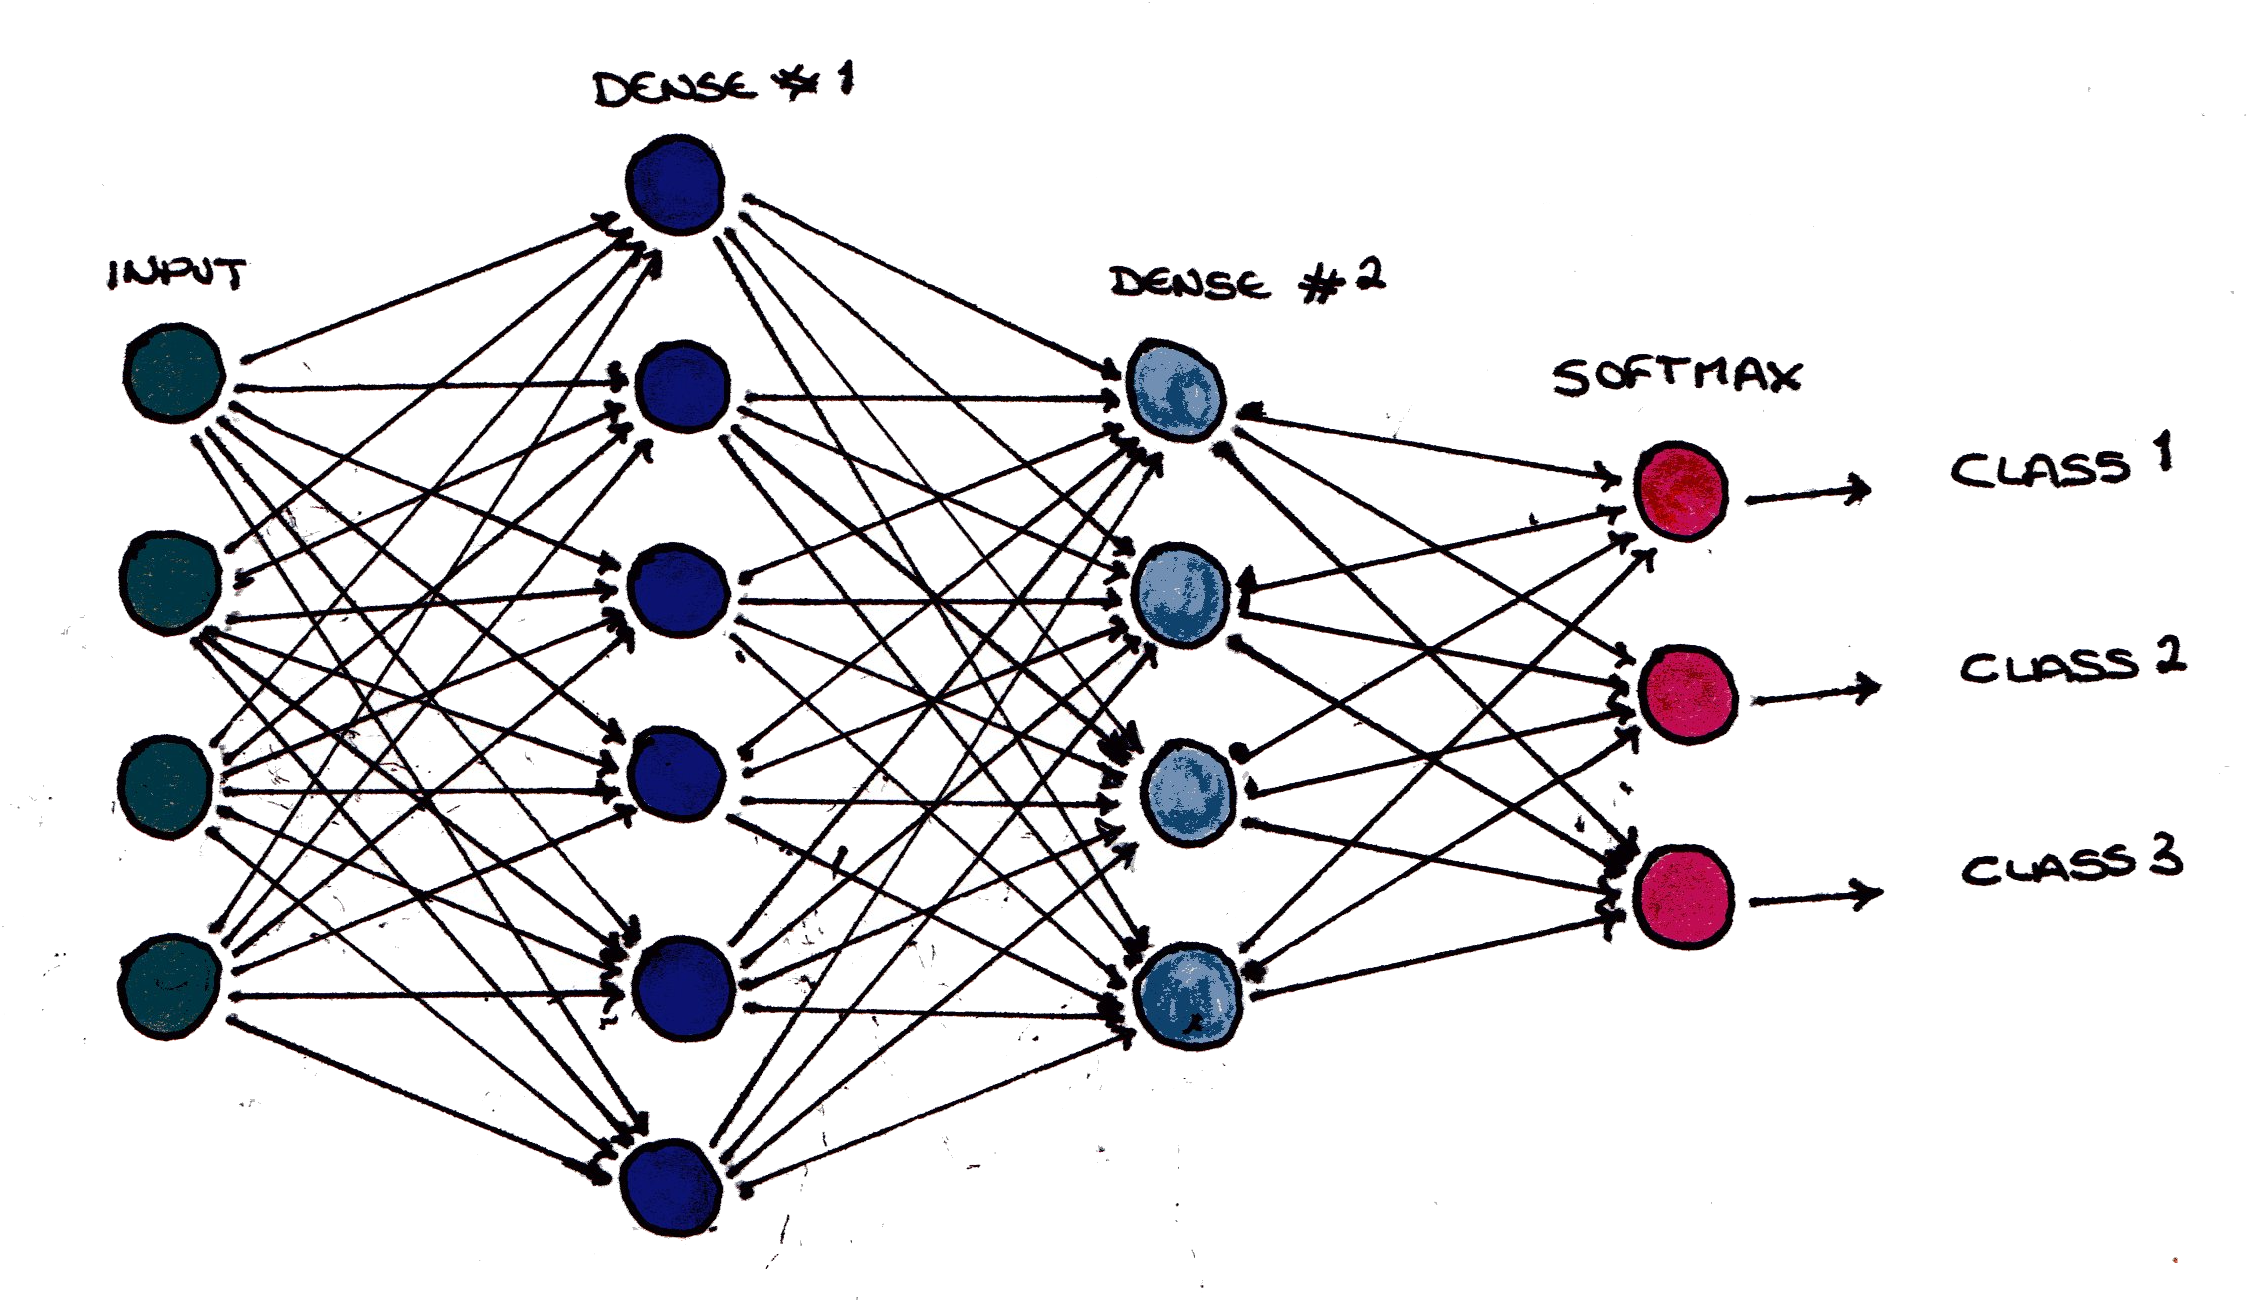
\includegraphics[width=1.0\linewidth]{figures/background_fully_connected.png}
                            
%                    \captionsetup{singlelinecheck=false, justification=raggedright}
%                    \caption{Graphical representation of . On the left .} \label{fig:neural_network_architecture_fully_connected}
%                \end{figure}
                
%                \begin{figure}
%                    \centering
                            
%                    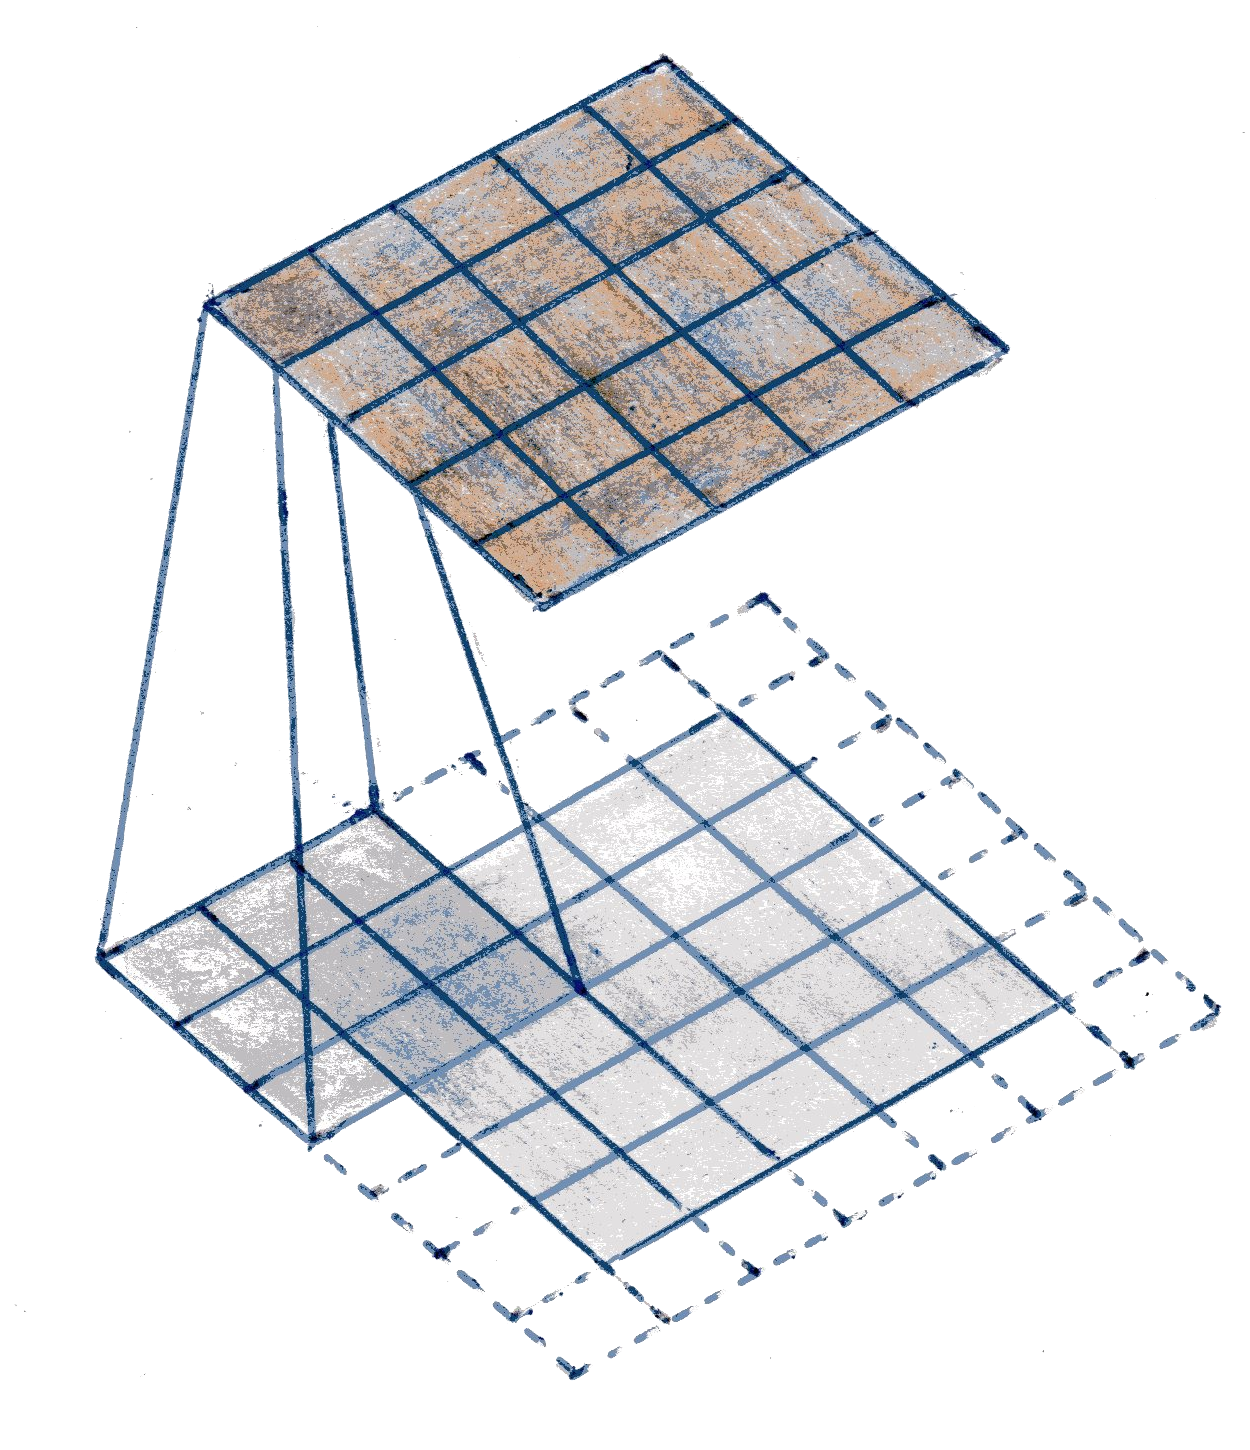
\includegraphics[width=1.0\linewidth]{figures/background_cnn.png}
                            
%                    \captionsetup{singlelinecheck=false, justification=raggedright}
%                    \caption{Graphical representation of . On the left .} \label{fig:neural_network_architecture_cnn}
%                \end{figure}
                
%                \begin{figure}
%                    \centering
                            
%                    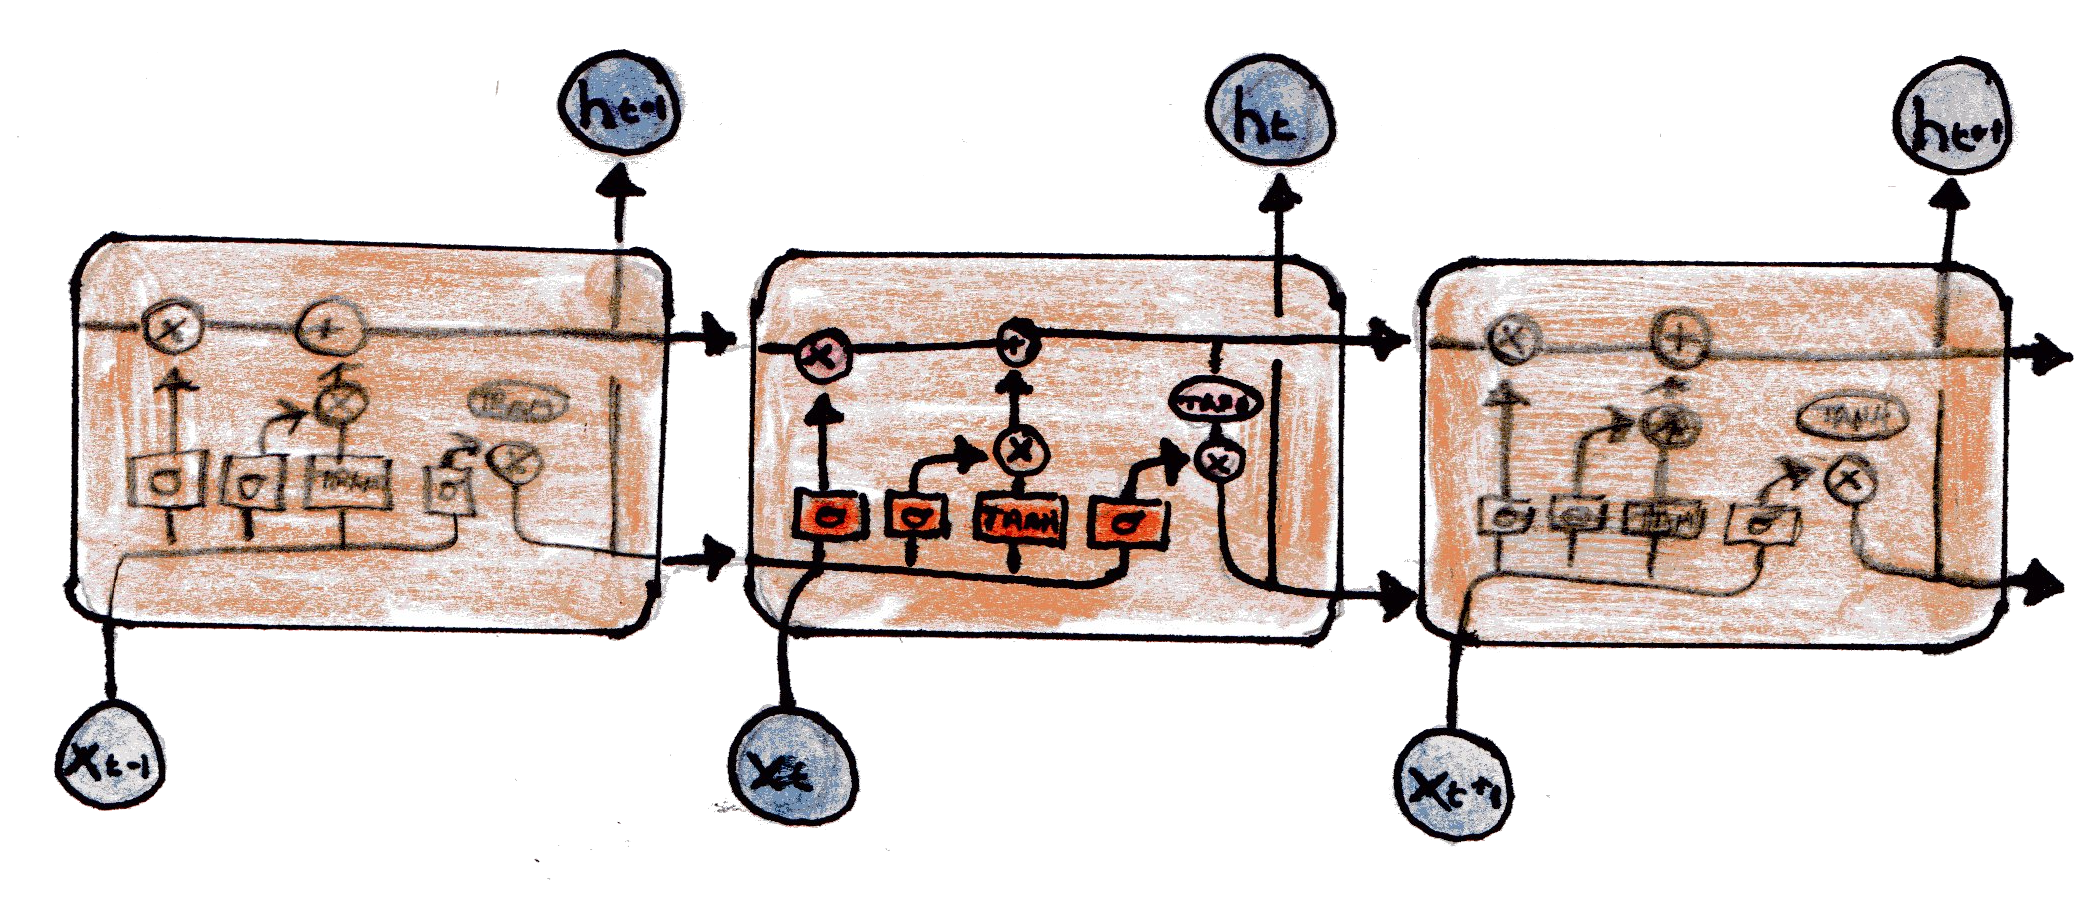
\includegraphics[width=1.0\linewidth]{figures/background_lstm.png}
                            
%                    \captionsetup{singlelinecheck=false, justification=raggedright}
%                    \caption{Graphical representation of . On the left .} \label{fig:neural_network_architecture_lstm}
%                \end{figure}
                
%            \subsubsection{Activation Function} \label{sec:activation_function}
%                \begin{figure}
%                    \centering
                            
%                    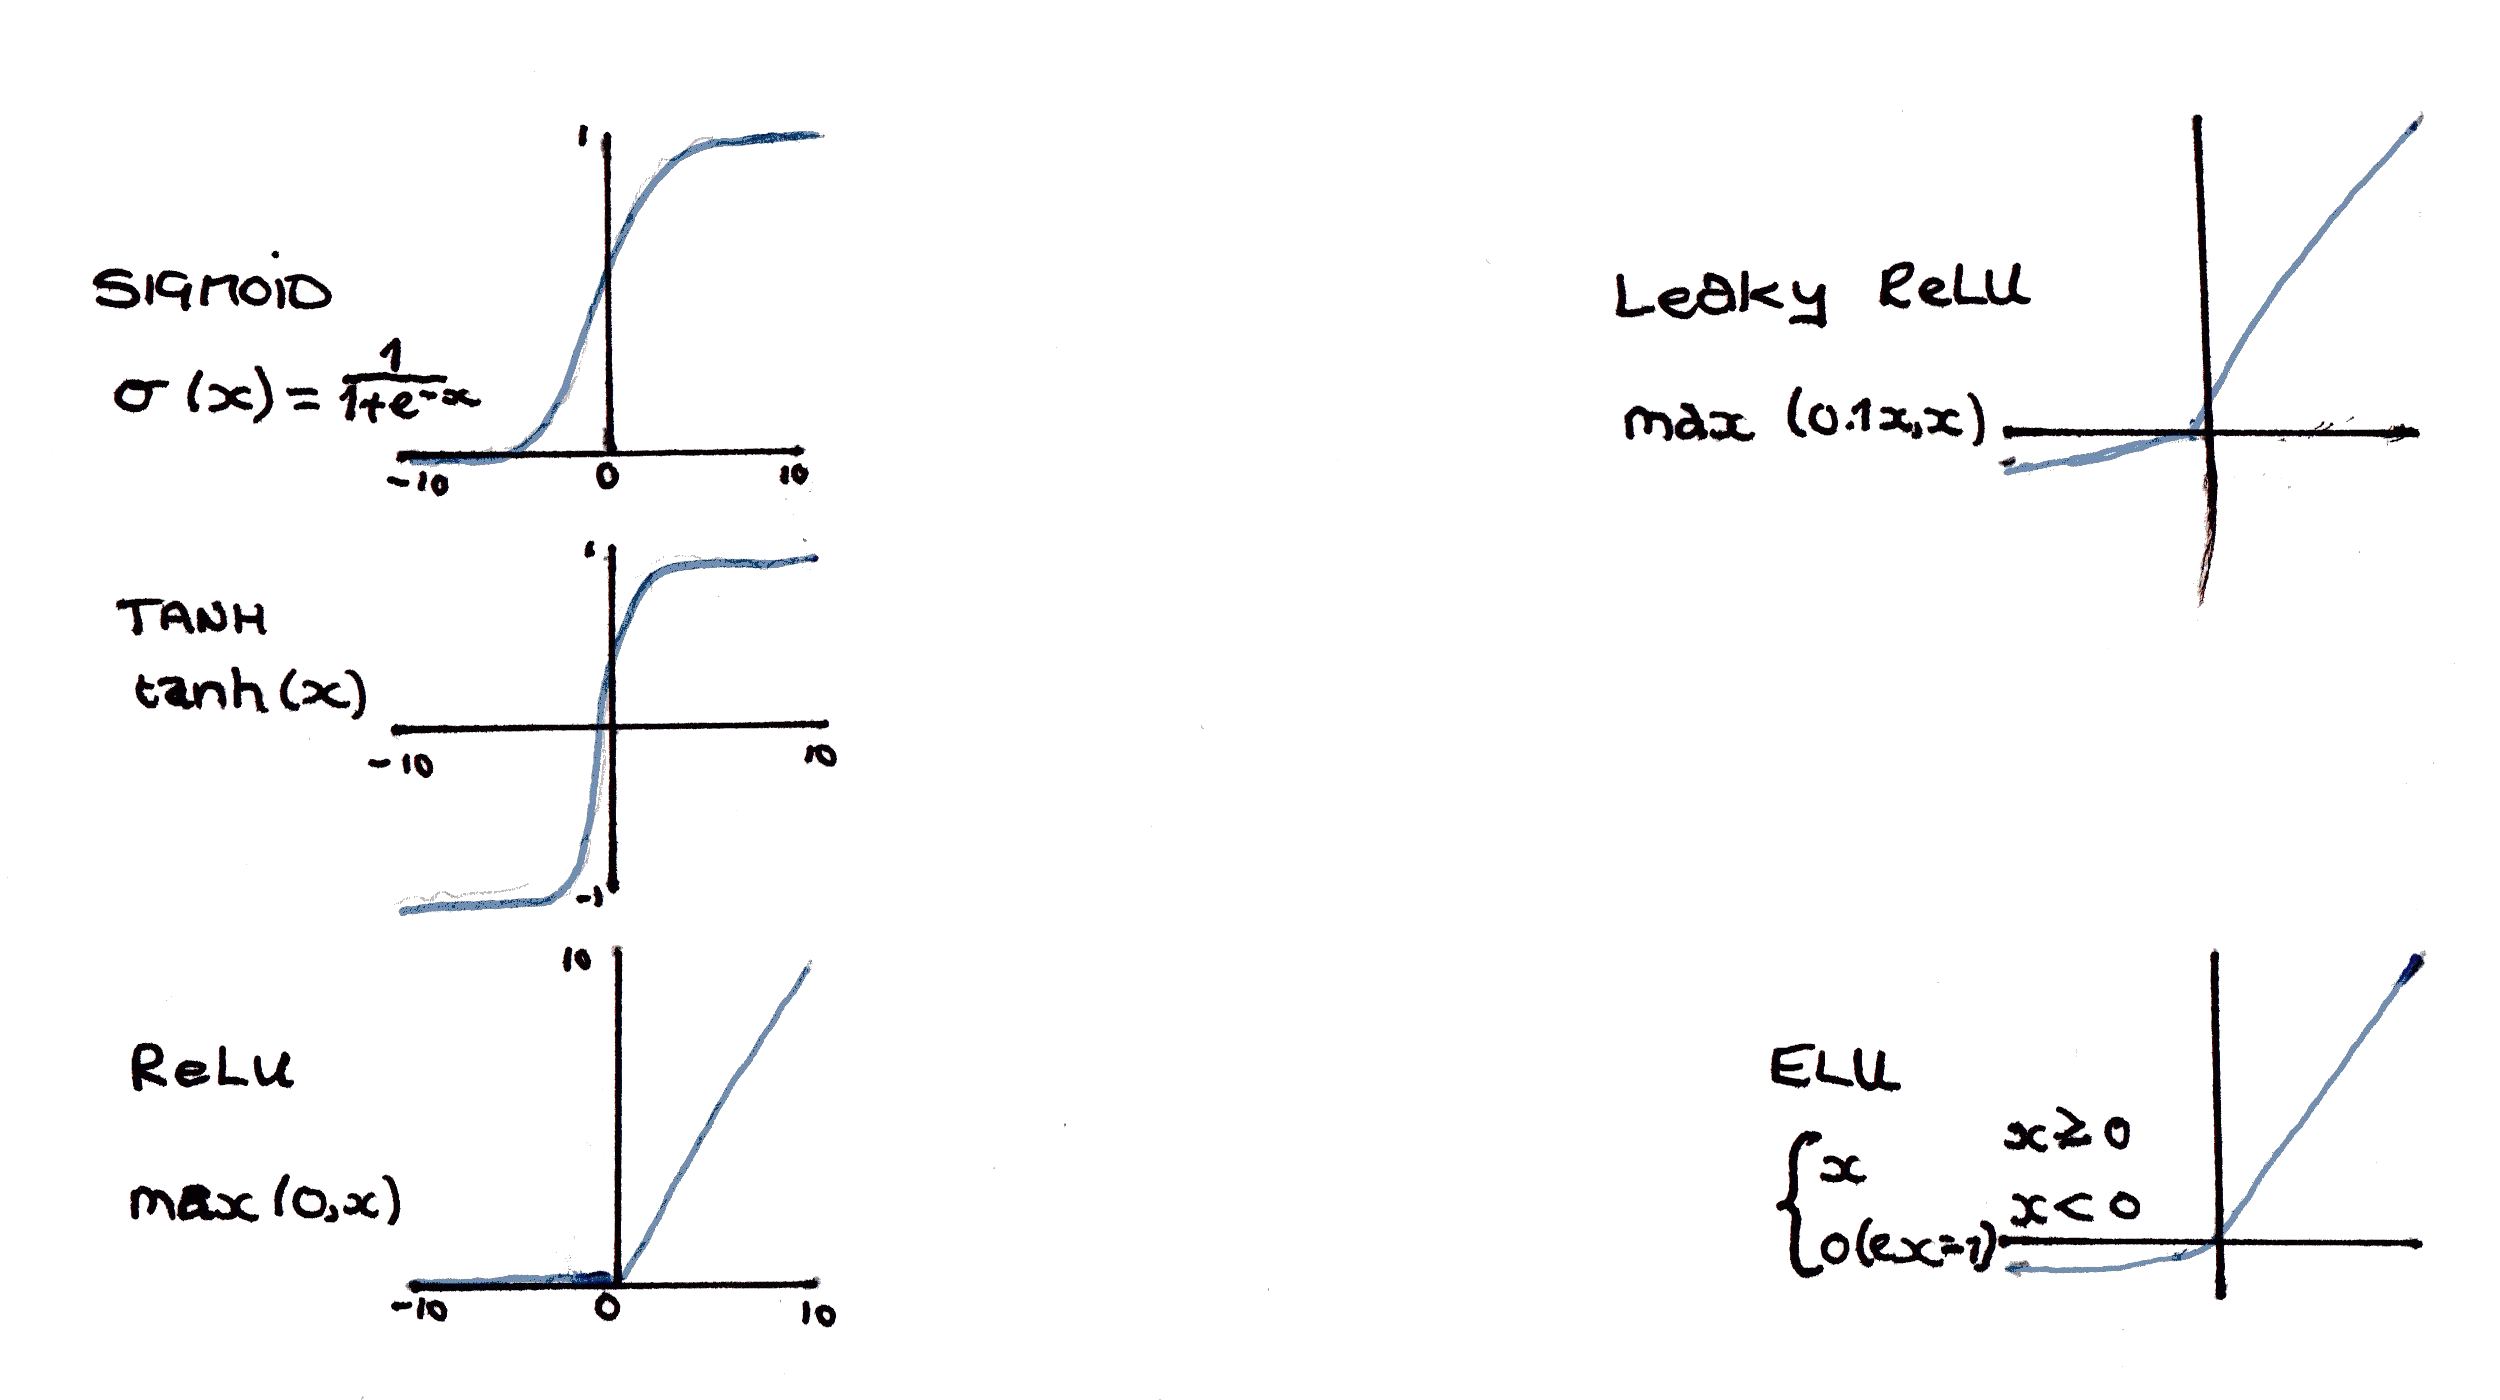
\includegraphics[width=1.0\linewidth]{figures/background_activation_functions.png}
                            
%                    \captionsetup{singlelinecheck=false, justification=raggedright}
%                    \caption{Graphical representation of . On the left .} \label{fig:activation_function_activation_functions}
%                \end{figure}
                
%                \begin{figure}
%                    \centering
                            
%                    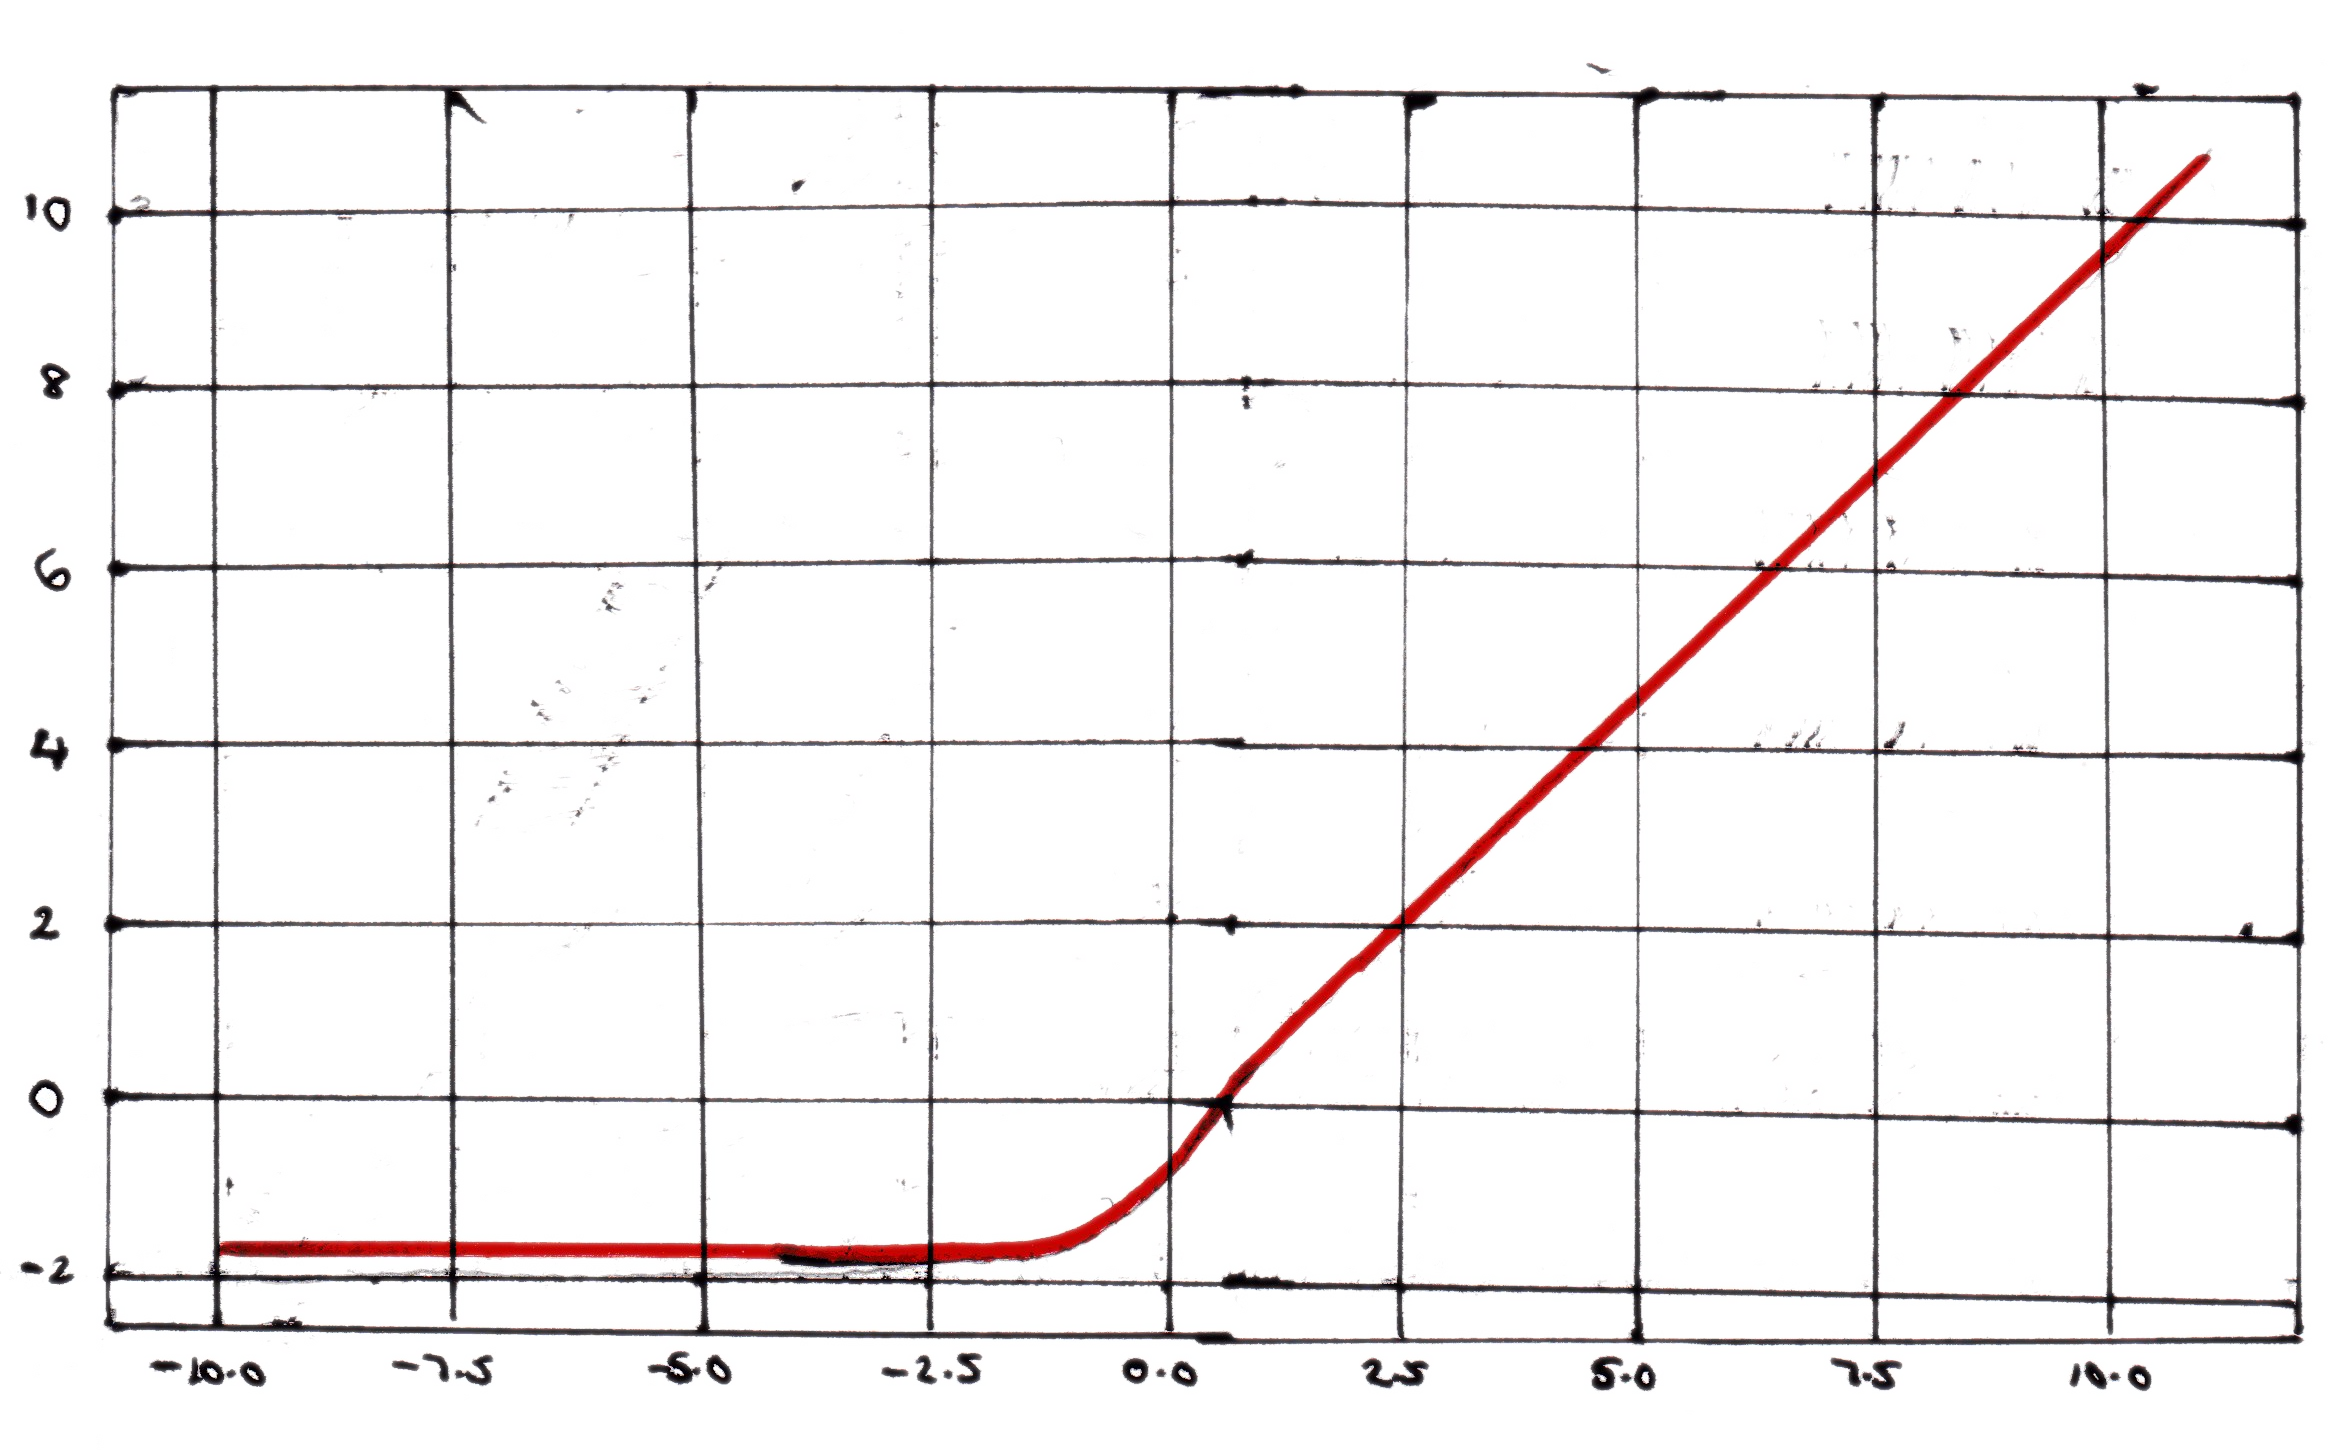
\includegraphics[width=1.0\linewidth]{figures/background_selu.png}
                            
%                    \captionsetup{singlelinecheck=false, justification=raggedright}
%                    \caption{Graphical representation of . On the left .} \label{fig:activation_function_selu}
%                \end{figure}
            
%            \subsubsection{Regularisation} \label{sec:regularisation}
%                \begin{figure}
%                    \centering
                            
%                    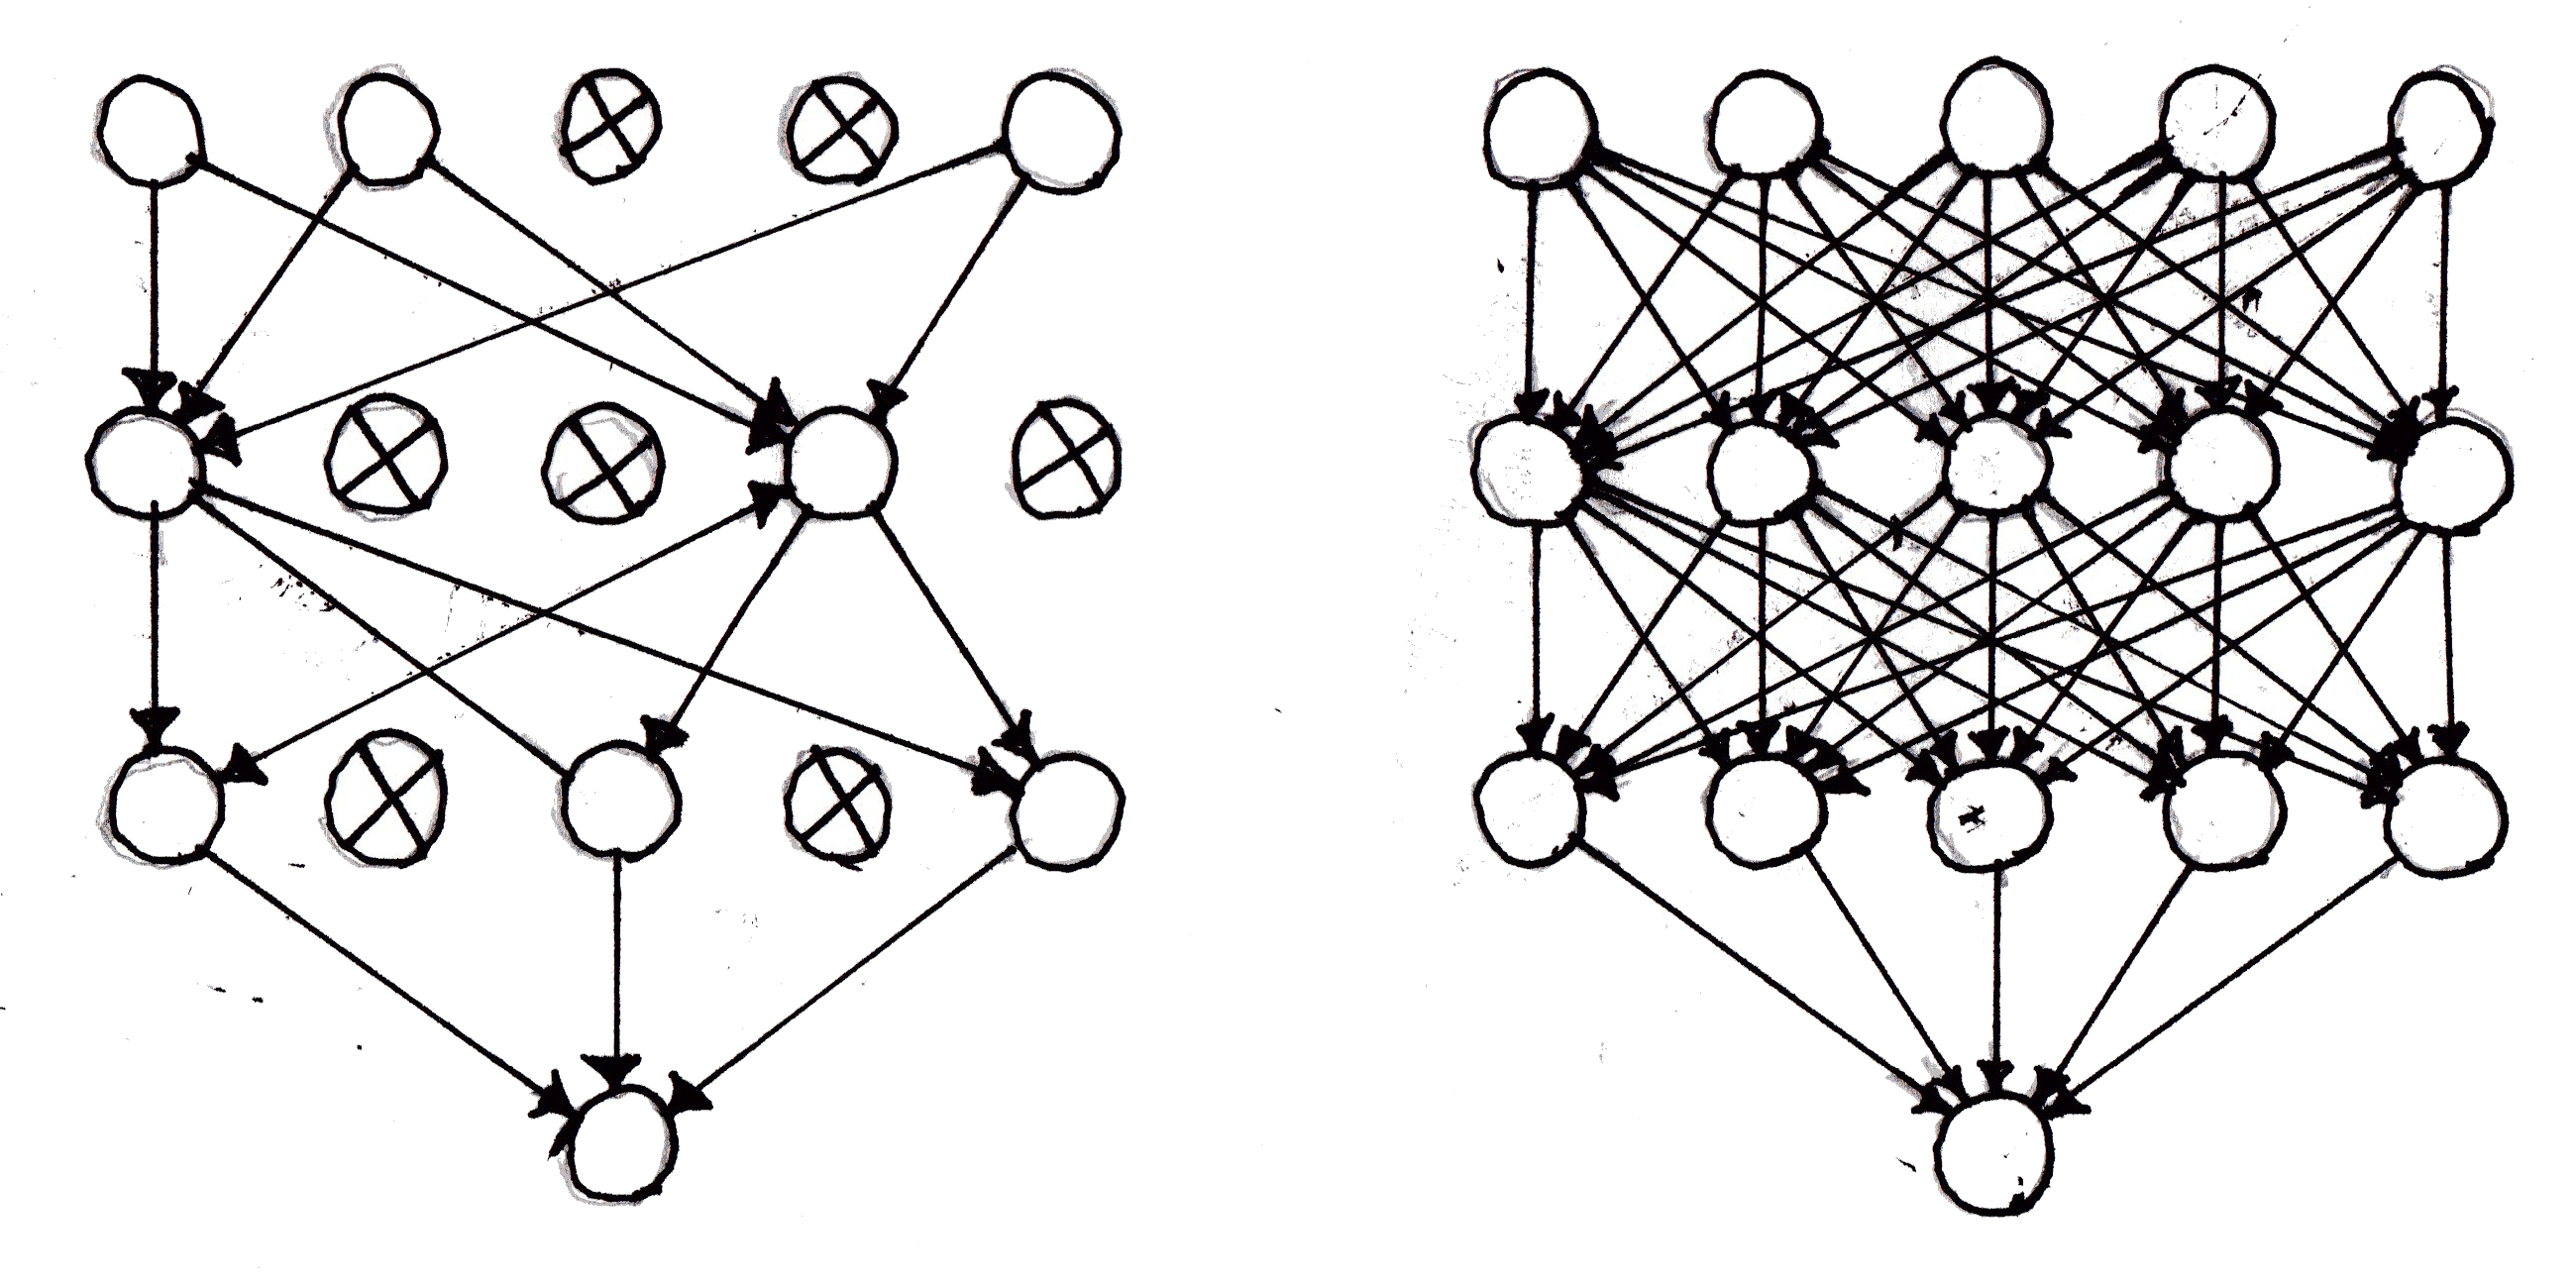
\includegraphics[width=1.0\linewidth]{figures/background_dropout.png}
                            
%                    \captionsetup{singlelinecheck=false, justification=raggedright}
%                    \caption{Graphical representation of . On the left .} \label{fig:regularisation_dropout}
%                \end{figure}
                
        
        % \subsection{Machine Learning for PET Image Reconstruction} \label{sec:machine_learning_for_pet_image_reconstruction}
            % might want to mention this?
            
        
%        \subsection{Machine Learning for Motion Correction} \label{sec:machine_learning_for_motion_correction}
            
